\documentclass[dvipsnames]{beamer}
\usepackage[utf8]{inputenc}
\usepackage{listings}
\usepackage{comment}
\usepackage{soul}
%\usepackage{ulem}
\usepackage{subfig}
\setul{}{1pt}
\usepackage[oldenum, olditem]{paralist}
%allow even smaller text
\newcommand\tinytiny{\fontsize{4pt}{3}\selectfont}

\makeatletter
\let\old@lstKV@SwitchCases\lstKV@SwitchCases
\def\lstKV@SwitchCases#1#2#3{}
\makeatother
\usepackage{lstlinebgrd}
\makeatletter
\let\lstKV@SwitchCases\old@lstKV@SwitchCases

\lst@Key{numbers}{none}{%
    \def\lst@PlaceNumber{\lst@linebgrd}%
    \lstKV@SwitchCases{#1}%
    {none:\\%
     left:\def\lst@PlaceNumber{\llap{\normalfont
                \lst@numberstyle{\thelstnumber}\kern\lst@numbersep}\lst@linebgrd}\\%
     right:\def\lst@PlaceNumber{\rlap{\normalfont
                \kern\linewidth \kern\lst@numbersep
                \lst@numberstyle{\thelstnumber}}\lst@linebgrd}%
    }{\PackageError{Listings}{Numbers #1 unknown}\@ehc}}
\makeatother


\graphicspath{{logos/}}

%disclaimer for Sandia. uncomment and the whole blob goes away @ b80c116300122
\def\sandid{SAND2020-7475 PE}

% \title{Performance Portability with Kokkos}
\title{The Kokkos Lectures}

%BAD misuse of author field
\author{The Compact Course}

%\author{
%  Jeff Miles \inst{1},
%  Christian Trott \inst{1}
%}
%\institute[shortinst]{\tiny \inst{1} Sandia National Laboratories, \inst{2} Oak Ridge National Laboratory \and \inst{3} Los Alamos National Laboratory}
%\institute[shortinst]{\tiny \inst{1} Sandia National Laboratories}

\usetheme{kokkos}

\newif\ifshort
\newif\ifmedium
\newif\iffull
\newif\ifnotoverview

\newcommand{\TutorialDirectory}{\texttt{Intro-Full}}
\newcommand{\ExerciseDirectory}[1]{\texttt{Exercises/#1/}}
\newcommand{\TutorialClone}{\texttt{Kokkos/kokkos-tutorials/\TutorialDirectory}}

\definecolor{darkgreen}{rgb}{0.0, 0.5, 0.0}
\definecolor{darkred}{rgb}{0.8, 0.0, 0.0}
\definecolor{orange}{rgb}{0.8, 0.33, 0.0}
\definecolor{purple}{rgb}{0.60, 0.20, 0.80}
\colorlet{bodyColor}{blue!20}
\colorlet{patternColor}{orange!30}
\colorlet{policyColor}{green!30}

% http://tex.stackexchange.com/questions/144448/color-a-text-line-in-a-code-lstlisting
\lstnewenvironment{code}[1][]%
{
  %with txfonts: OT1/txr/m/n/10
  %with default fonts: OT1/cmr/m/n/10
  %\fontfamily{cmr}\selectfont
  %\showthe\font
   \noindent
   \minipage{\linewidth}
   %\vspace{0.5\baselineskip}
   \lstset{mathescape, escapeinside={<@}{@>},
moredelim=**[is][{\btHL[fill=patternColor]}]{@pattern}{@pattern},
moredelim=**[is][{\btHL[fill=red!30]}]{@warning}{@warning},
moredelim=**[is][{\btHL[fill=policyColor]}]{@policy}{@policy},
moredelim=**[is][{\btHL[fill=bodyColor]}]{@body}{@body},
moredelim=**[is][{\btHL[fill=red!30]}]{@warning}{@warning},
moredelim=**[is][\color{black}]{@black}{@black},
moredelim=**[is][\color{blue}]{@blue}{@blue},
moredelim=**[is][\bf]{@bold}{@bold},
moredelim=**[is][\it]{@italic}{@italic},
moredelim=**[is][\color{boldblue}\bf]{@boldblue}{@boldblue},
moredelim=**[is][\color{red}]{@red}{@red},
moredelim=**[is][\color{green}]{@green}{@green},
moredelim=**[is][\color{gray}]{@gray}{@gray},
moredelim=**[is][\color{darkgreen}]{@darkgreen}{@darkgreen},
moredelim=**[is][\color{darkred}]{@darkred}{@darkred},
moredelim=**[is][\color{orange}]{@orange}{@orange},
moredelim=**[is][\color{purple}]{@purple}{@purple},
keywords={},
#1}
}
{
  \endminipage
  %\vspace{1.0\baselineskip}
}

\makeatletter
\newif\ifATOlinebackground
\lst@Key{linebackground}{\tiny}{\def\ATOlinebackground{#1}\global\ATOlinebackgroundtrue}
\makeatother

\lstnewenvironment{shell}[1][]{%
  \global\ATOlinebackgroundfalse
  \lstset{language=sh,%
    showstringspaces=false,
    aboveskip=0pt,
    frame=none,
    numbers=none,
    belowskip=2pt,
    breaklines=true,
    #1,
    }
  %\ifATOlinebackground
  \lstset{linebackgroundcolor={
    \ATOlinebackground
  }}
  %\fi
  }{}

\lstnewenvironment{cmake}[1][]{%
  \global\ATOlinebackgroundfalse
  \lstset{language=sh,%
    showstringspaces=false,
    aboveskip=0pt,
    frame=none,
    numbers=none,
    belowskip=2pt,
    breaklines=true,
    #1,
    }
  %\ifATOlinebackground
  \lstset{linebackgroundcolor={
    \ATOlinebackground
  }}
  %\fi
  }{}

\newcommand{\inlinecode}[1]{{\lstset{basicstyle=\ttfamily,keywordstyle={},showstringspaces=false}\lstinline$#1$}}
\newcommand{\inlineshell}[1]{{\lstset{basicstyle=\ttfamily,keywordstyle={},showstringspaces=false}\lstinline$#1$}}

\setbeamercolor{block title}{fg=white, bg=SandiaLightBlue}
\setbeamercolor{block body}{bg=lightgray}
\setbeamercolor{block title alerted}{fg=white, bg=SandiaRed}
\setbeamercolor{block body alerted}{bg=lightgray}



%\usepackage[texcoord,grid,gridunit=mm,gridcolor=red!10,subgridcolor=green!10]{eso-pic}
\usepackage[absolute,overlay]{textpos}





% http://tex.stackexchange.com/questions/8851/how-can-i-highlight-some-lines-from-source-code

\usepackage{pgf, pgffor}
\usepackage{listings}
\usepackage{lstlinebgrd} % see http://www.ctan.org/pkg/lstaddons

\makeatletter
%%%%%%%%%%%%%%%%%%%%%%%%%%%%%%%%%%%%%%%%%%%%%%%%%%%%%%%%%%%%%%%%%%%%%%%%%%%%%%
%
% \btIfInRange{number}{range list}{TRUE}{FALSE}
%
% Test in int number <number> is element of a (comma separated) list of ranges
% (such as: {1,3-5,7,10-12,14}) and processes <TRUE> or <FALSE> respectively

\newcount\bt@rangea
\newcount\bt@rangeb

\newcommand\btIfInRange[2]{%
    \global\let\bt@inrange\@secondoftwo%
    \edef\bt@rangelist{#2}%
    \foreach \range in \bt@rangelist {%
        \afterassignment\bt@getrangeb%
        \bt@rangea=0\range\relax%
        \pgfmathtruncatemacro\result{ ( #1 >= \bt@rangea) && (#1 <= \bt@rangeb) }%
        \ifnum\result=1\relax%
            \breakforeach%
            \global\let\bt@inrange\@firstoftwo%
        \fi%
    }%
    \bt@inrange%
}
\newcommand\bt@getrangeb{%
    \@ifnextchar\relax%
        {\bt@rangeb=\bt@rangea}%
        {\@getrangeb}%
}
\def\@getrangeb-#1\relax{%
    \ifx\relax#1\relax%
        \bt@rangeb=100000%   \maxdimen is too large for pgfmath
    \else%
        \bt@rangeb=#1\relax%
    \fi%
}

%%%%%%%%%%%%%%%%%%%%%%%%%%%%%%%%%%%%%%%%%%%%%%%%%%%%%%%%%%%%%%%%%%%%%%%%%%%%%%
%
% \btLstHL<overlay spec>{range list}
%
% TODO BUG: \btLstHL commands can not yet be accumulated if more than one overlay spec match.
%
\newcommand<>{\btLstHL}[2]{%
  \only#3{\btIfInRange{\value{lstnumber}}{#1}{\color{#2}\def\lst@linebgrdcmd{\color@block}}{\def\lst@linebgrdcmd####1####2####3{}}}%
}%
\makeatother






% http://tex.stackexchange.com/questions/15237/highlight-text-in-code-listing-while-also-keeping-syntax-highlighting
%\usepackage[T1]{fontenc}
%\usepackage{listings,xcolor,beramono}
\usepackage{tikz}

\makeatletter
\newenvironment{btHighlight}[1][]
{\begingroup\tikzset{bt@Highlight@par/.style={#1}}\begin{lrbox}{\@tempboxa}}
{\end{lrbox}\bt@HL@box[bt@Highlight@par]{\@tempboxa}\endgroup}

\newcommand\btHL[1][]{%
  \begin{btHighlight}[#1]\bgroup\aftergroup\bt@HL@endenv%
}
\def\bt@HL@endenv{%
  \end{btHighlight}%
  \egroup
}
\newcommand{\bt@HL@box}[2][]{%
  \tikz[#1]{%
    \pgfpathrectangle{\pgfpoint{1pt}{0pt}}{\pgfpoint{\wd #2}{\ht #2}}%
    \pgfusepath{use as bounding box}%
    \node[anchor=base west, fill=orange!30,outer sep=0pt,inner xsep=1pt, inner ysep=0pt, rounded corners=3pt, minimum height=\ht\strutbox+1pt,#1]{\raisebox{1pt}{\strut}\strut\usebox{#2}};
  }%
}
\makeatother



\usetikzlibrary{calc}
\usepackage{xparse}%  For \NewDocumentCommand

% tikzmark command, for shading over items
\newcommand{\tikzmark}[1]{\tikz[overlay,remember picture] \node (#1) {};}

\makeatletter
\NewDocumentCommand{\DrawBox}{s O{}}{%
    \tikz[overlay,remember picture]{
    \IfBooleanTF{#1}{%
        \coordinate (RightPoint) at ($(left |- right)+(\linewidth-\labelsep-\labelwidth,0.0)$);
    }{%
        \coordinate (RightPoint) at (right.east);
    }%
    \draw[red,#2]
      ($(left)+(-0.2em,0.9em)$) rectangle
      ($(RightPoint)+(0.2em,-0.3em)$);}
}

\NewDocumentCommand{\DrawBoxWide}{s O{}}{%
    \tikz[overlay,remember picture]{
    \IfBooleanTF{#1}{%
        \coordinate (RightPoint) at ($(left |- right)+(\linewidth-\labelsep-\labelwidth,0.0)$);
    }{%
        \coordinate (RightPoint) at (right.east);
    }%
    \draw[red,#2]
      ($(left)+(-\labelwidth,0.9em)$) rectangle
      ($(RightPoint)+(0.2em,-0.3em)$);}
}

\NewDocumentCommand{\DrawBoxWideBlack}{s O{}}{%
    \tikz[overlay,remember picture]{
    \IfBooleanTF{#1}{%
        \coordinate (RightPoint) at ($(left |- right)+(\linewidth-\labelsep-\labelwidth,0.0)$);
    }{%
        \coordinate (RightPoint) at (right.east);
    }%
    \draw[black,#2]
      ($(left)+(-\labelwidth,0.9em)$) rectangle
      ($(RightPoint)+(0.2em,-0.3em)$);}
}
\makeatother

\usetikzlibrary{positioning}

\usetikzlibrary{shapes}

\hypersetup{
    colorlinks=true,
    linkcolor=blue,
    filecolor=magenta,
    urlcolor=cyan,
}



\shorttrue
\mediumtrue
\fullfalse

\begin{document}


\begin{frame}
	\titlepage
\end{frame}

\begin{frame}{The Compact Course}
	{\huge The Compact Course}

	\textbf{A 1-Day Tutorial}

	\vspace{10pt}
	This lecture covers many concepts of Kokkos with Hands-On Exercises as homework.

	Slides: \url{https://github.com/kokkos/kokkos-tutorials/Intro-Medium/KokkosTutorial_Medium.pdf}

	\vspace{20pt}
	For the full lectures, with more capabilities covered, and more in-depth explanations visit:

	\url{https://github.com/kokkos/kokkos-tutorials/wiki/Kokkos-Lecture-Series}
\end{frame}


% \begin{frame}{DOE ECP Acknowledgement}

% \textit{
% This research was supported by the Exascale Computing Project (17-SC-20-SC),
% a joint project of the U.S. Department of Energy’s Office of Science and National Nuclear Security Administration,
% responsible for delivering a capable exascale ecosystem, including software, applications, and hardware technology,
% to support the nation’s exascale computing imperative. 
% }

% \end{frame}

%==============================================================================
\ifnotoverview
\begin{frame}[fragile]

  \vspace{-10pt}

  {\Huge Introduction}

  \vspace{10pt}

  \textbf{Learning objectives:}
  \begin{itemize}
    \item{Why do we need Kokkos}
    \item{The Kokkos Ecosystem}
    \item{The Kokkos Team}
  \end{itemize}

  \vspace{-20pt}

\end{frame}
\fi

\begin{frame}[fragile]{The HPC Hardware Landscape}
  \begin{center}
    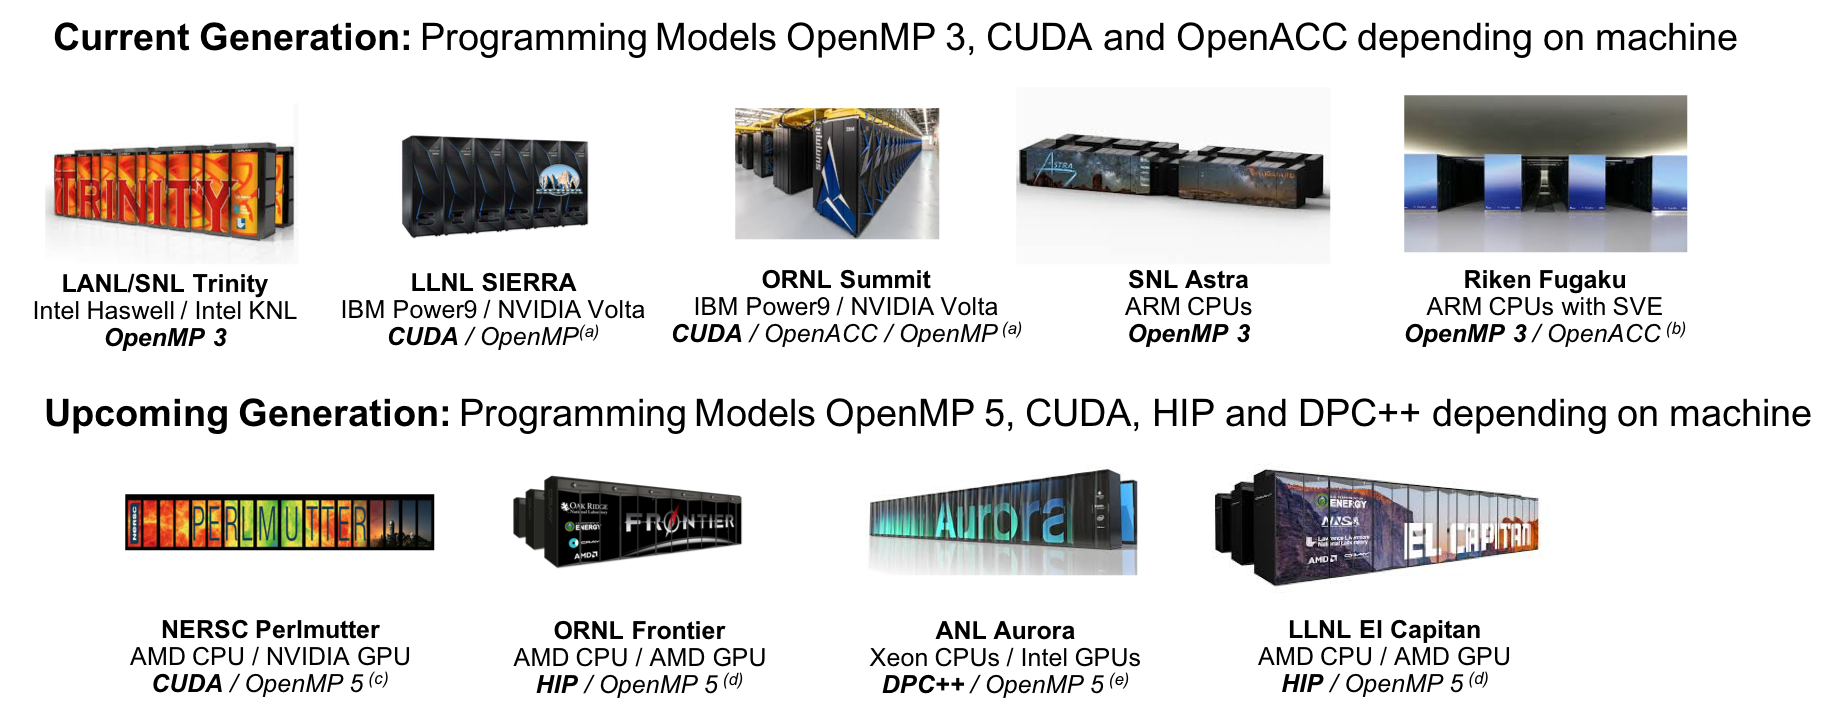
\includegraphics[width=1.05\textwidth]{figures/Architecture-Overview}
  \end{center}

  \begin{scriptsize}
  \emph{(a)} Initially not working. Now more robust for Fortran than C++, but getting better.

  \emph{(b)} Research effort.

  \emph{(c)} OpenMP 5 by NVIDIA.

  \emph{(d)} OpenMP 5 by HPE.

  \emph{(e)} OpenMP 5 by Intel.
  \end{scriptsize}

\end{frame}

\begin{frame}[fragile]{Cost of Coding}

\begin{block}{Industry Estimate}
A full time software engineer writes 10 lines of production code per hour: 20k LOC/year.
\end{block}

	\begin{itemize}
		\item Typical HPC production app: 300k-600k lines
			\begin{itemize}
				\item Sandia alone maintains a few dozen
			\end{itemize}
		\item Large Scientific Libraries:
			\begin{itemize}
				\item E3SM: 1,000k lines
				\item Trilinos: 4,000k lines
			\end{itemize}
	\end{itemize}

	\textbf{Conservative estimate:} need to rewrite 10\% of an app to switch Programming Model

	\pause

\begin{block}{Software Cost Switching Vendors}
Just switching Programming Models costs multiple person-years per app!
\end{block}

\end{frame}

\begin{frame}[fragile]{What is Kokkos?}
	\begin{itemize}
		\item A C++ Programming Model for Performance Portability
			\begin{itemize}
				\item Implemented as a template library on top CUDA, HIP, OpenMP, ...
				\item Aims to be descriptive not prescriptive
				\item Aligns with developments in the C++ standard
			\end{itemize}
		\item Expanding solution for common needs of modern science and engineering codes
			\begin{itemize}
				\item Math libraries based on Kokkos
				\item Tools for debugging, profiling and tuning
				\item Utilities for integration with Fortran and Python
			\end{itemize}
		\item It is an Open Source project with a growing community
			\begin{itemize}
				\item Maintained and developed at \url{https://github.com/kokkos}
				\item Hundreds of users at many large institutions
			\end{itemize}
	\end{itemize}
\end{frame}

\begin{frame}[fragile]{Kokkos at the Center}
  \begin{center}
    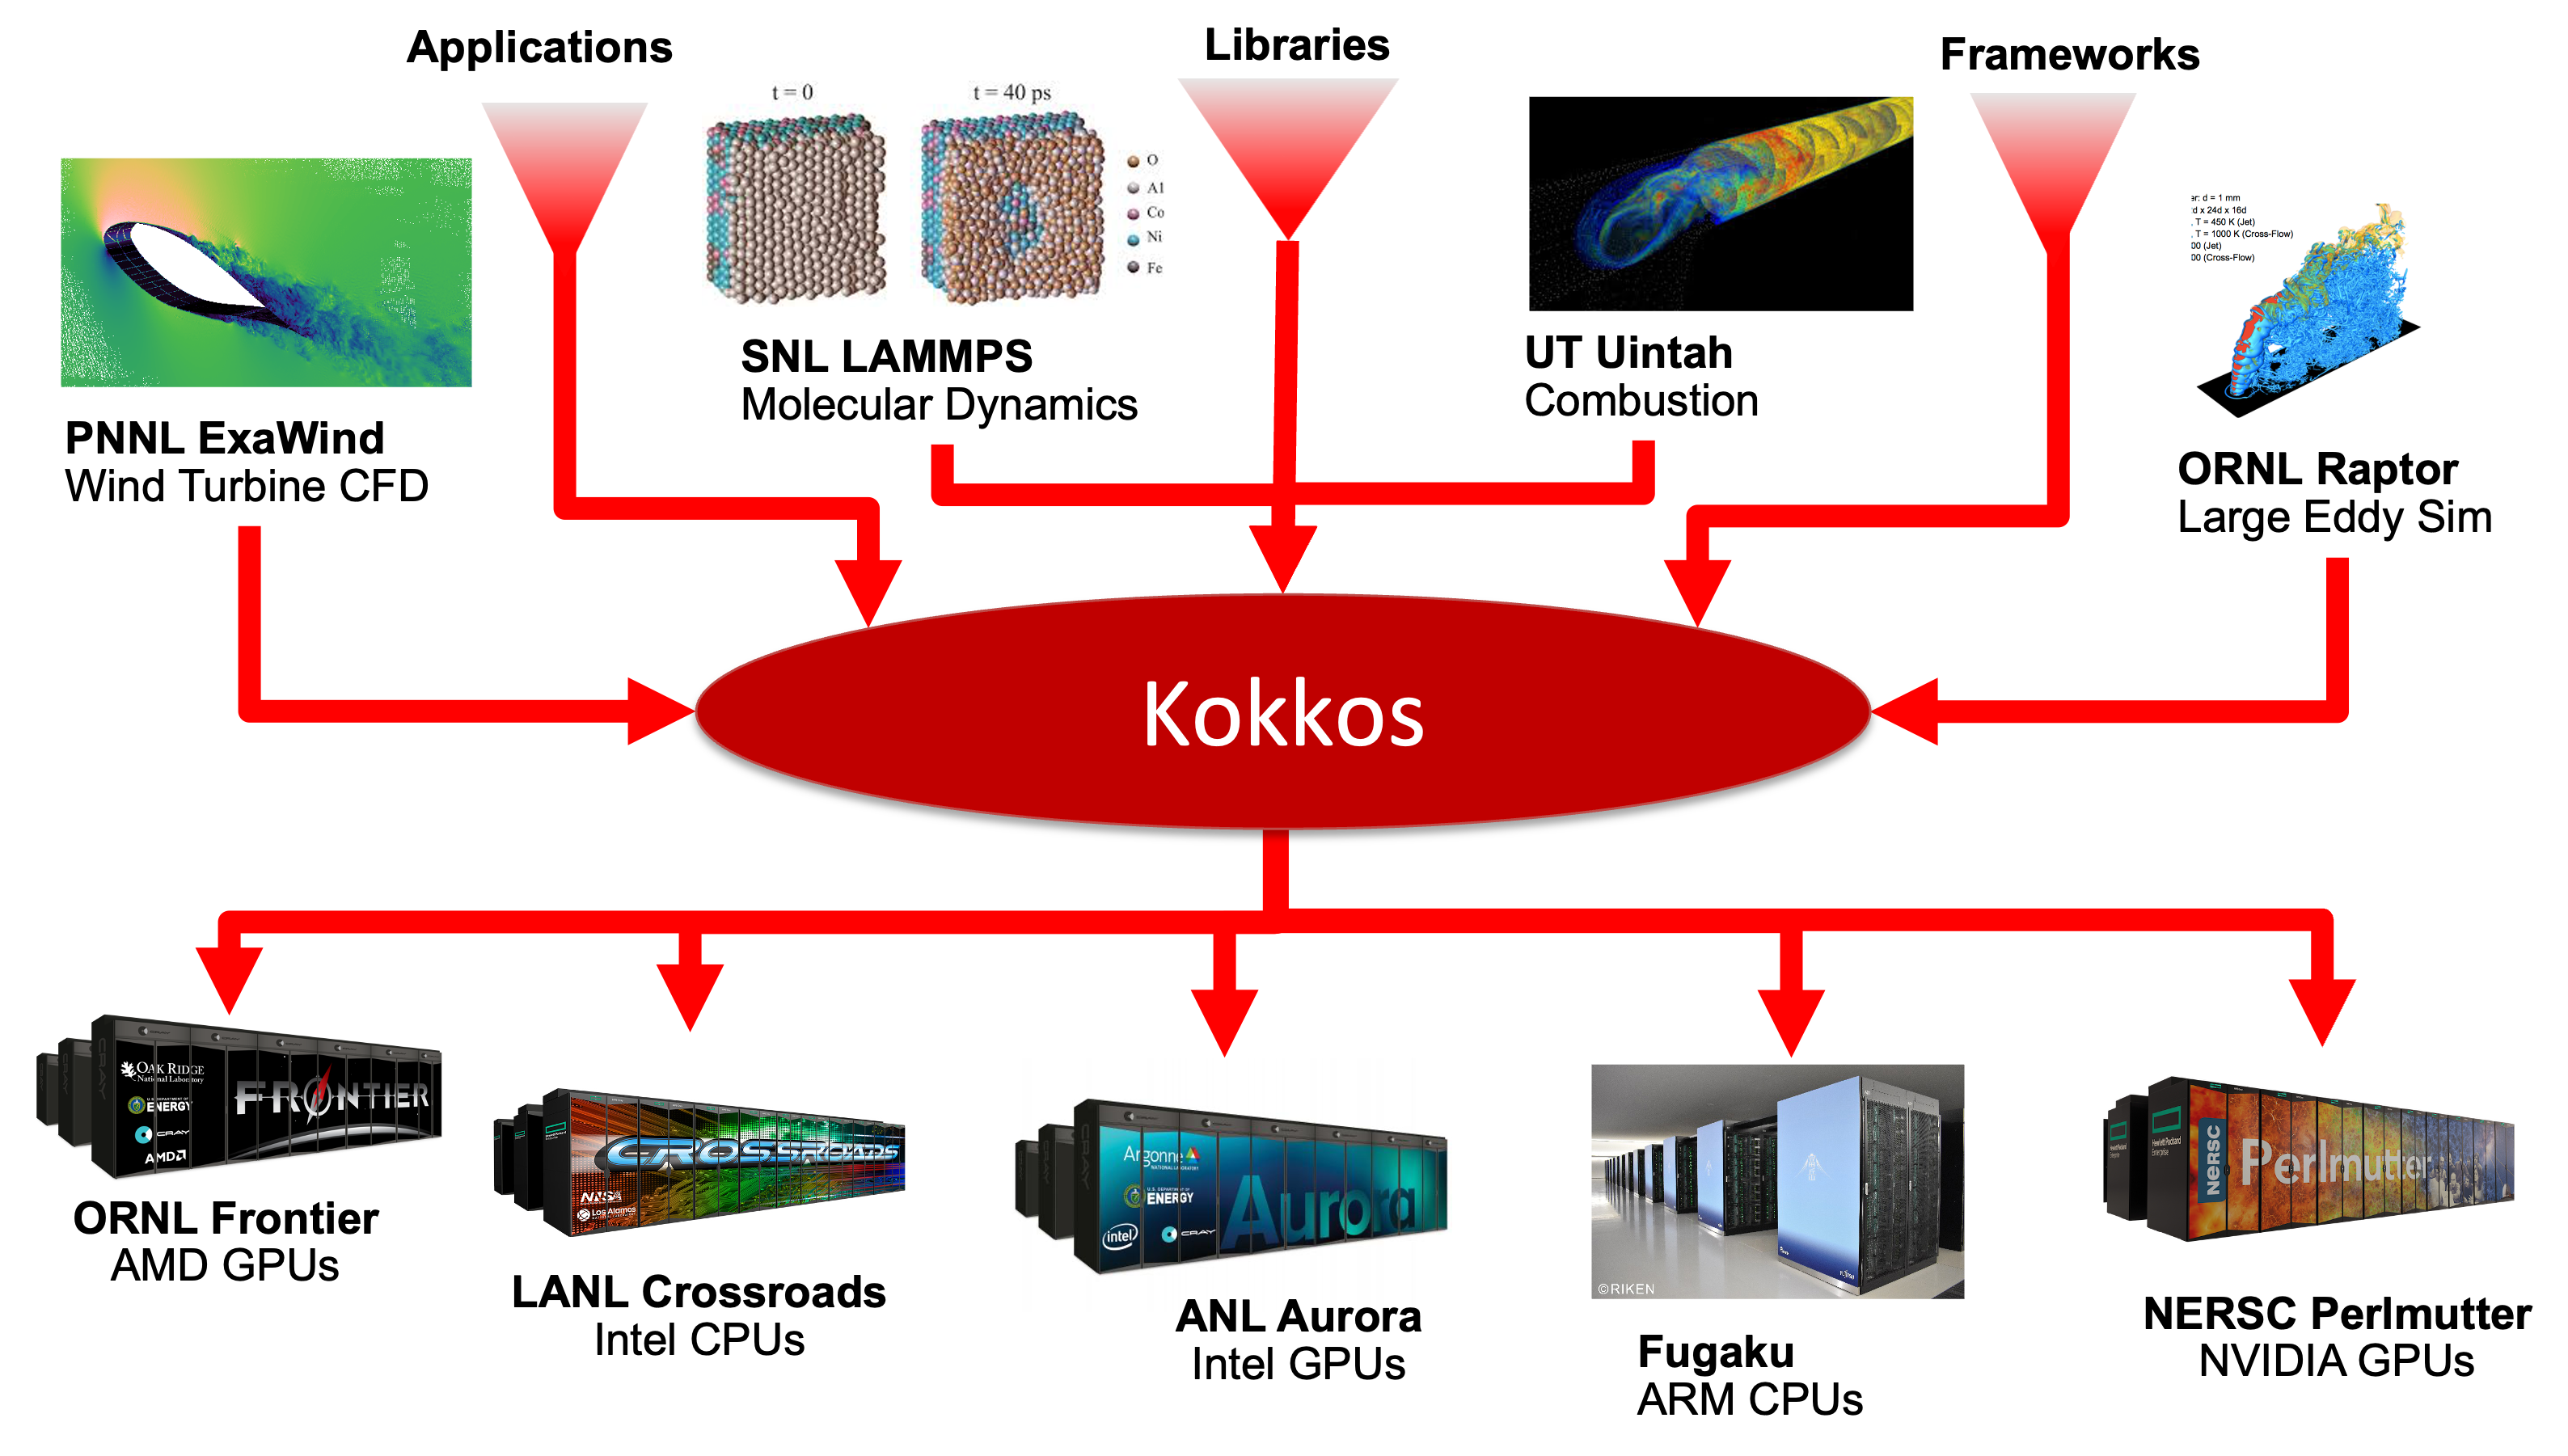
\includegraphics[width=1.05\textwidth]{figures/Kokkos-In-The-Middle-2024}
  \end{center}
\end{frame}

\begin{frame}[fragile]{The Kokkos Ecosystem}
  \begin{center}
    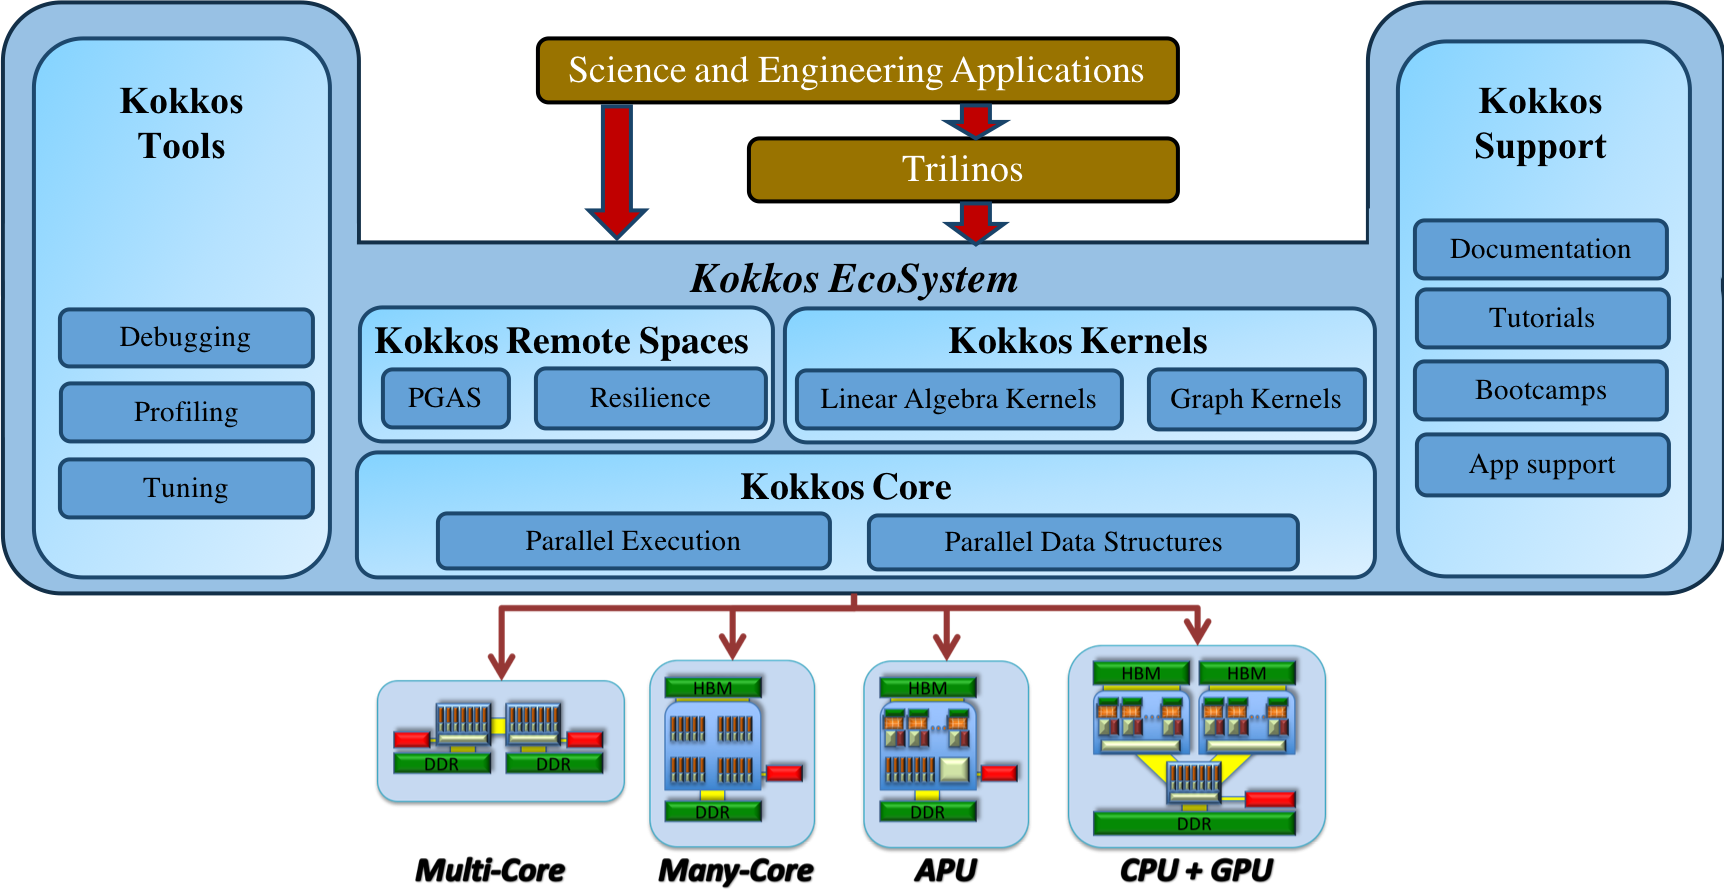
\includegraphics[width=1.05\textwidth]{figures/kokkos-eco-system}
  \end{center}
\end{frame}

\begin{frame}[fragile]{The Kokkos Team}
  \begin{center}
    
\includegraphics[width=0.9\textwidth]{figures/Kokkos-Team-2024}
  \end{center}
\end{frame}


\begin{frame}[fragile]{Kokkos and the C++ Standard}
  \textbf{Kokkos helps improve ISO C++}


	\vspace{-25pt}
\begin{center}                                                                                                                                    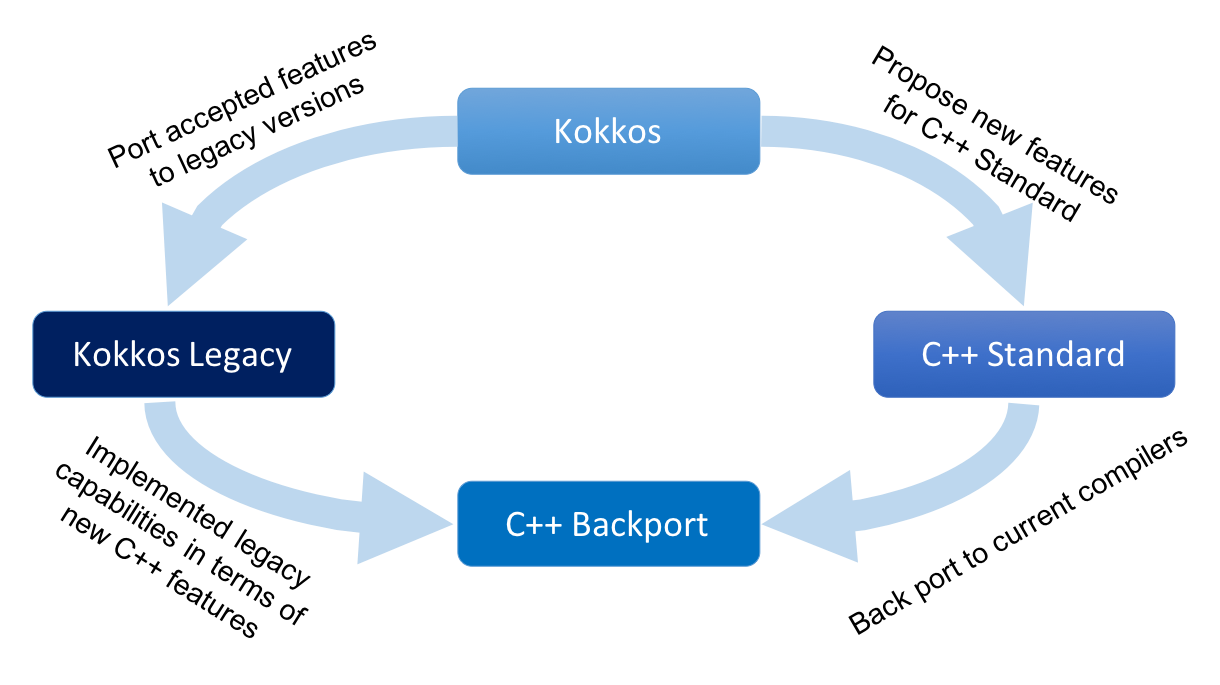
\includegraphics[width=1.05\textwidth]{figures/kokkos-cpp-standard}
\end{center}

	\vspace{-25pt}
\textit{Ten current or former Kokkos team members are members of the ISO C++ standard committee.}
\end{frame}

\iffull
\begin{frame}[fragile]{C++20 std::atomic\_ref}
	\textbf{C++11 std::atomic insufficient for HPC}
	\begin{itemize}
           \item Objects, not functions, with only atomic access
	   \item Can't use non-atomic access in one operation, and then atomic access in the next
	\end{itemize}

	\textbf{C++20 std::atomic\_ref adds atomic capabilites as in Kokkos}
	\begin{itemize}
		\item Can wrap standard allocations.
		\item Works also for sizes which can't be done lock-free (e.g. \texttt{complex$<$double$>$})
		\item Atomic operations on reasonably arbitrary types
	\end{itemize}

  \begin{code}[linebackgroundcolor={
      },
      keywords={atomic_add,atomic_ref}, frame=single
    ]
// Kokkos today
Kokkos::atomic_add(&a[i],5.0);

// atomic_ref in ISO C++20
std::atomic_ref(a[i]) += 5.0;
  \end{code}
\end{frame}
\fi

\iffull
\begin{frame}[fragile]{C++23 std::mdspan}
   \textbf{C++ does not provide multi dimensional arrays}
	\begin{itemize}
           \item Every scientific programming language has them: Fortran, Matlab, Python, ... 
	\end{itemize}

	\textbf{C++23 std::mdspan adds Kokkos::View like arrays}
	\begin{itemize}
		\item Reference semantics.
		\item Compile time and runtime extents (also mixed)
		\item Data layouts to allow for adapting hardware specific access patterns. 
		\item Subviews!
	\end{itemize}

  \begin{code}[linebackgroundcolor={
      },
      keywords={View,LayoutLeft,extents,mdspan,dynamic_extent,layout_left}, frame=single
    ]
// Kokkos today
View<float**[5],LayoutLeft> a("A",10,12); a(3,5,1) = 5;

// mdspan in ISO C++23
using ext = extents<int,dynamic_extent,dynamic_extent,5>;
mdspan<float,ext,layout_left> a(ptr,10,12); a[3,5,1]+=5;
  \end{code}

\end{frame}
\fi

\begin{frame}{Kokkos Users}
\textbf{Kokkos has a growing OpenSource Community}

\vspace{0.5cm}
\begin{itemize}
  \item 20 ECP projects list Kokkos as Critical Dependency
    \begin{itemize}
       \item 41 list C++ as critical
       \item 25 list Lapack as critical
       \item 21 list Fortran as critical
    \end{itemize}
  \item Slack Channel: 1.7k members from 100+ institutions
    \begin{itemize}
      \item 15\% Sandia Nat. Lab.
      \item 24\% other US Labs
      \item 22\% universities
      \item 39\% other
    \end{itemize}
  \item GitHub: 1.9k stars
\end{itemize}

\begin{tikzpicture}[remember picture,overlay]
    \node[xshift=-3.5cm,yshift=-6.5cm] at (current page.north east){%
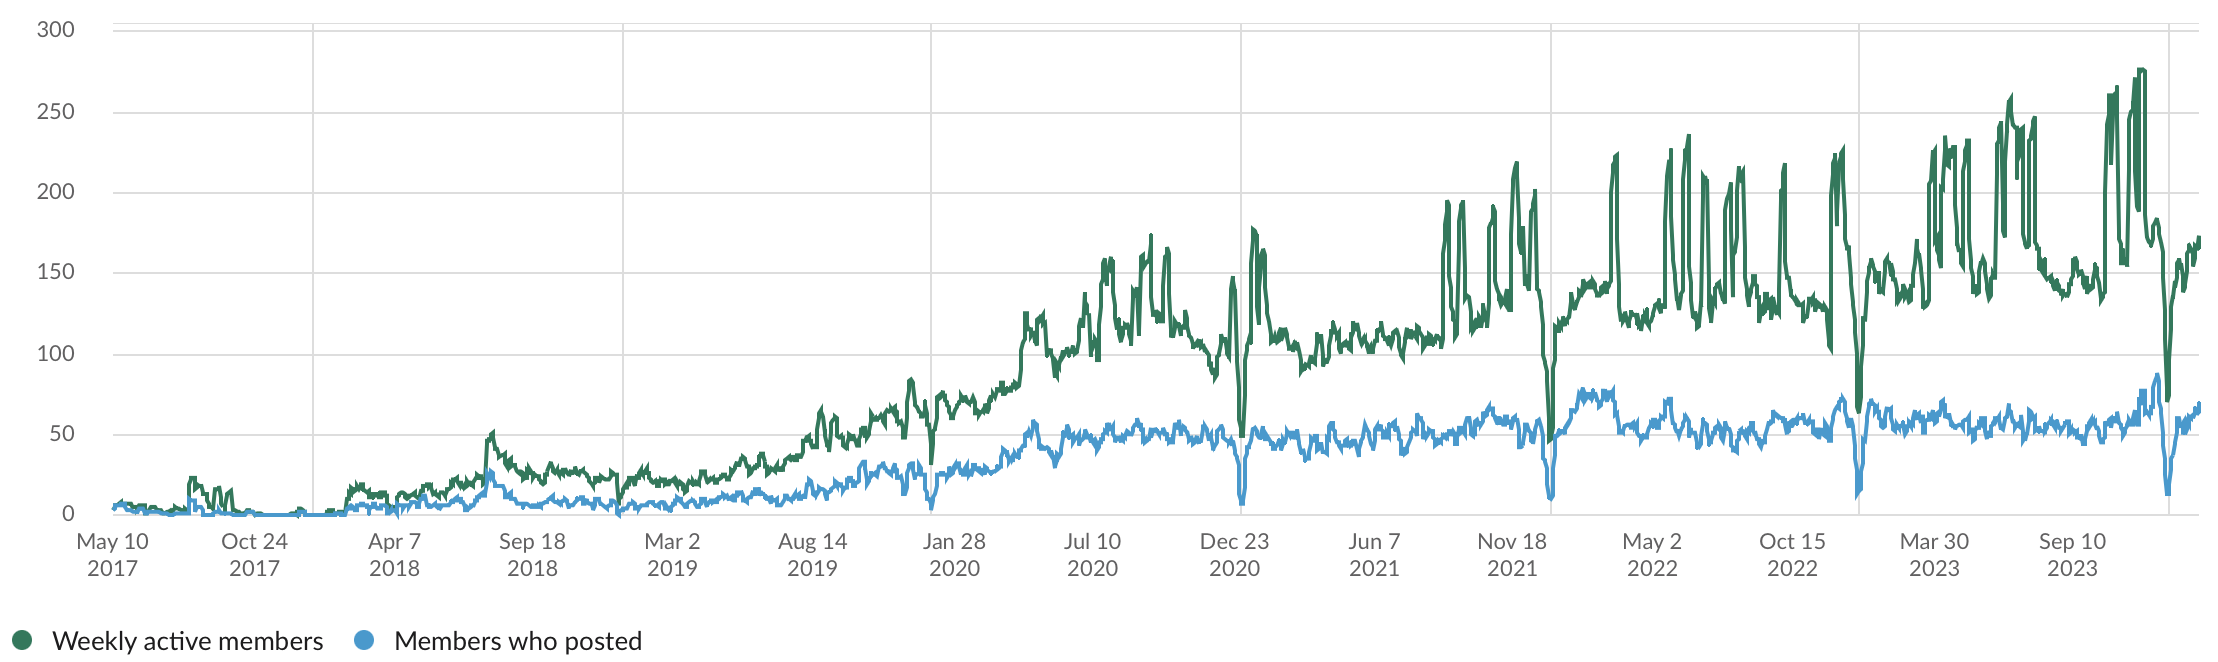
\includegraphics[width=6cm]{figures/KokkosSlack-Users-Feb24}
};
\end{tikzpicture}


\end{frame}


\begin{frame}{Welcome to Kokkos}

\textbf{Online Resources}:

\begin{itemize}
        \item \url{https://github.com/kokkos}:
                \begin{itemize}
                        \item Primary Kokkos GitHub Organization
                \end{itemize}
        \item \url{https://github.com/kokkos/kokkos-tutorials/wiki/Kokkos-Lecture-Series}:
                \begin{itemize}
			\item{Slides, recording and Q\&A for the Full Lectures}
                \end{itemize}
        \item \url{https://github.com/kokkos/kokkos/wiki}:
                \begin{itemize}
                        \item Wiki including API reference
                \end{itemize}
        \item \url{https://kokkosteam.slack.com}:
                \begin{itemize}
                        \item Slack channel for Kokkos.
                        \item Please join: fastest way to get your questions answered.
                        \item Can whitelist domains, or invite individual people.
                \end{itemize}
\end{itemize}

\end{frame}

%==========================================================================

\begin{frame}[fragile]{}

  {\Huge Data parallel patterns}

  \vspace{20pt}

  \textbf{Learning objectives:}
  \begin{itemize}
    \item{How computational bodies are passed to the Kokkos runtime.}
    \item{How work is mapped to execution resources.}
    \item{The difference between \texttt{parallel\_for} and \texttt{parallel\_reduce}.}
    \item{Start parallelizing a simple example.}
  \end{itemize}

  \vspace{-20pt}

\end{frame}

%==========================================================================

\begin{frame}[fragile]{Using Kokkos for data parallel patterns (0)}

  \textbf{\ul{Data parallel patterns and work}}

  \begin{code}[linebackgroundcolor={
        \btLstHL<1->{2}{bodyColor}
      }
    ]
@patternfor@pattern (atomIndex = @policy0; atomIndex < numberOfAtoms; ++atomIndex@policy) {
  atomForces[atomIndex] = calculateForce(...data...);
}
  \end{code}

  Kokkos maps \textbf{work} to execution resources

  \pause

  \begin{itemize}
    \item {each iteration of a computational body is a \textbf{unit of work}.}
    \item {an \textbf{iteration index} identifies a particular unit of work.}
    \item {an \textbf{iteration range} identifies a total amount of work.}
  \end{itemize}

  \pause

  \vspace{0pt}

  \begin{block}{Important concept: Work mapping}
    You give an \textbf{iteration range} and \textbf{computational body} (kernel) \\
    to Kokkos, and Kokkos decides how to map that work to execution resources.
  \end{block}

  \vspace{-10pt}

\end{frame}

%==========================================================================

\begin{frame}[fragile]{Using Kokkos for data parallel patterns (2)}

  \textbf{How are computational bodies given to Kokkos?}

  \vspace{6pt}
  \pause

  \hspace{10pt} As \textbf{functors} or \textit{function objects}, a common pattern in C++.

  \pause
  \vspace{10pt}

  Quick review, a \textbf{functor} is a function with data. Example:
  \begin{code}[keywords={}, frame=single]
struct @darkredParallelFunctor@darkred {
  ...
  void operator()( <@\emph{a work assignment}@> ) const {
    @body/* ... computational body ... */@body
  ...
};
  \end{code}

\end{frame}

%==========================================================================

\begin{frame}[fragile]{Using Kokkos for data parallel patterns (3)}

  \textbf{How is work assigned to functor operators?}

  \vspace{6pt}
  \pause

  \hspace{10pt} A total amount of work items is given to a Kokkos pattern,
  \begin{code}[keywords={}, frame=single]
@darkredParallelFunctor@darkred @bluefunctor@blue;
@patternKokkos::parallel_for@pattern(@policynumberOfIterations@policy, @bluefunctor@blue);
  \end{code}

  \vspace{0pt}
  \pause

  \hspace{10pt} and work items are assigned to functors one-by-one:

  \begin{code}[keywords={}, frame=single]
@graystruct Functor {
  void operator()(@gray@blackconst int64_t index@black@gray) const {...}
}@gray
  \end{code}

  \pause
  \vspace{5pt}

  \begin{alertblock}{Warning: concurrency and order}
    Concurrency and ordering of parallel iterations is \textit{not} guaranteed by the Kokkos runtime.
  \end{alertblock}

  \vspace{0pt}

\end{frame}

%==========================================================================

\iffull
\begin{frame}[fragile]{Using Kokkos for data parallel patterns (4)}

  \textbf{How is data passed to computational bodies?}

  \vspace{2pt}

  \begin{code}
for (atomIndex = 0; atomIndex < numberOfAtoms; ++atomIndex) {
  @darkgreenatomForces@darkgreen[atomIndex] = calculateForce(@darkred...data...@darkred);
}
  \end{code}

  \vspace{-3pt}

  \begin{code}[keywords={}, frame=single]
@graystruct AtomForceFunctor {
  ...
  void operator()(const int64_t atomIndex) const {@gray
    @darkgreenatomForces@darkgreen[atomIndex] = calculateForce(@darkred...data...@darkred);
  @gray}
  ...
}@gray
  \end{code}
  \pause
  \vspace{5pt}

  How does the body access the data?

  \vspace{-3pt}

  \begin{block}{Important concept}
    A parallel functor body must have access to all the data it needs through the functor's \textbf{data members}.
  \end{block}

\end{frame}
\fi

%==========================================================================

\iffull
\begin{frame}[fragile]{Using Kokkos for data parallel patterns (5)}

  \textbf{\ul{Putting it all together: the complete functor}}:

  \begin{code}[keywords={}, frame=single]
struct AtomForceFunctor {
  <@\emph{ForceType}@> @darkgreen_atomForces;@darkgreen
  <@\emph{DataType}@> @darkred_atomData;@darkred
  AtomForceFunctor(/* args */) {...}
  void operator()(const int64_t atomIndex) const {
    @darkgreen_atomForces@darkgreen[atomIndex] = calculateForce(@darkred_atomData@darkred);
  }
};
  \end{code}

  \vspace{5pt}
  \pause

  \textbf{Q/} How would we \textbf{reproduce serial execution} with this functor?

  \vspace{3pt}

  \begin{code}[keywords={}, frame=single]
for (atomIndex = 0; atomIndex < numberOfAtoms; ++atomIndex){
  @darkgreenatomForces@darkgreen[atomIndex] = calculateForce(@darkreddata@darkred);
}
  \end{code}

  \begin{textblock*}{0.5\textwidth}(0.05\textwidth,0.600\textheight)
    \only<2->{\rotatebox{90}{\textbf{Serial}}}
  \end{textblock*}

  %\vspace{3pt}
  \pause

  \begin{code}[keywords={}, frame=single]
AtomForceFunctor @bluefunctor@blue(@darkgreenatomForces@darkgreen, @darkreddata@darkred);
for (atomIndex = 0; atomIndex < numberOfAtoms; ++atomIndex){
  @bluefunctor@blue(atomIndex);
}
  \end{code}

  \begin{textblock*}{0.5\textwidth}(0.05\textwidth,0.755\textheight)
    \only<3->{\rotatebox{90}{\textbf{Functor}}}
  \end{textblock*}

\end{frame}
\fi

%==========================================================================

\begin{frame}[fragile]{Using Kokkos for data parallel patterns (6)}

  \textbf{\ul{The complete picture}} (using functors):

  \vspace{8pt}

  1.  Defining the functor (operator+data):

  \vspace{0pt}

  \begin{code}[keywords={}, frame=single]
struct AtomForceFunctor {
  <@\emph{ForceType}@> @darkgreen_atomForces;@darkgreen
  <@\emph{DataType}@> @darkred_atomData;@darkred

  AtomForceFunctor(<@\emph{ForceType}@> atomForces, <@\emph{DataType}@> data) :
    @darkgreen_atomForces@darkgreen(atomForces), @darkred_atomData@darkred(data) {}

  void operator()(const int64_t atomIndex) const {
    @body@darkgreen_atomForces@darkgreen[atomIndex] = calculateForce(@darkred_atomData@darkred);@body
  }
}
  \end{code}

  \vspace{5pt}

  2.  \textbf{Executing} in parallel with Kokkos pattern:

  \vspace{-4pt}

  \begin{code}
AtomForceFunctor functor(atomForces, data);
@patternKokkos::parallel_for@pattern(@policynumberOfAtoms@policy, functor);
  \end{code}

\end{frame}

%==========================================================================

\begin{frame}[fragile]{Using Kokkos for data parallel patterns (7)}

  Functors are tedious $\Rightarrow$ \ul{\textbf{C++11 Lambdas} are concise}

  \vspace{5pt}

  \begin{code}[linebackgroundcolor={
        \btLstHL<1->{4-6}{black!15}
      },
      keywords={}, frame=single]
@grayatomForces already exists
data already exists
Kokkos::parallel_for(numberOfAtoms, @gray
    [=] (const int64_t atomIndex) {
    @darkgreenatomForces@darkgreen[atomIndex] = calculateForce(@darkreddata@darkred);
  }
@gray);@gray
  \end{code}

  \pause

  A lambda is not \textit{magic}, it is the compiler \textbf{auto-generating} a \textbf{functor} for you.

  \pause
  \vspace{7pt}

  \begin{alertblock}{Warning: Lambda capture and C++ containers}
    For portability to GPU a lambda must capture by value \texttt{[=]}. \\
    Don't capture containers (\textit{e.g.}, std::vector)
    by value because it will copy the container's entire contents.
  \end{alertblock}

  %\pause
  %$\Rightarrow$ So, {\color{darkgreen}\texttt{atomForces}} must be a pointer (e.g., not a \texttt{std::vector})

\end{frame}

%==========================================================================

\begin{frame}[fragile]{parallel\_for examples}

  \textbf{How does this compare to OpenMP?}

  \vspace{5pt}

  \begin{code}[linebackgroundcolor={
      },
      frame=single
    ]
for (int64_t i = 0; i < N; ++i) {
  /* loop body */
}
  \end{code}

  \begin{code}[linebackgroundcolor={
        \btLstHL<1->{3}{bodyColor}
      },
      frame=single
    ]
#pragma @policyomp parallel@policy @patternfor@pattern
@patternfor@pattern (int64_t i = @policy0; i < N@policy; ++i) {
  /* loop body */
}
  \end{code}

  \begin{code}[linebackgroundcolor={
        \btLstHL<1->{2}{bodyColor}
      },
      frame=single
    ]
@patternparallel_for@pattern(@policyN@policy, [=] (const int64_t i) {
  /* loop body */
});
  \end{code}


  \begin{textblock*}{0.5\textwidth}(0.05\textwidth,0.200\textheight)
    \rotatebox{90}{\textbf{Serial}}
  \end{textblock*}

  \begin{textblock*}{0.5\textwidth}(0.05\textwidth,0.350\textheight)
    \rotatebox{90}{\textbf{OpenMP}}
  \end{textblock*}

  \begin{textblock*}{0.5\textwidth}(0.05\textwidth,0.550\textheight)
    \rotatebox{90}{\textbf{Kokkos}}
  \end{textblock*}


  \begin{block}{Important concept}
    Simple Kokkos usage is \textbf{no more conceptually difficult} than OpenMP, the annotations just go in different places.
  \end{block}

\end{frame}

%==========================================================================

\begin{frame}[fragile]{Scalar integration (0)}

  \textbf{\ul{Riemann-sum-style numerical integration}}:

  \vspace{-20pt}

  \begin{columns}[t,onlytextwidth]
    \column{.50\textwidth}
      \vspace{10pt}
      \[y = \int_{\textcolor{darkred}{lower}}^{\textcolor{blue}{upper}} {\textcolor{darkgreen}{function}}(x)\,dx\]
    \column{.50\textwidth}
      \begin{center}
      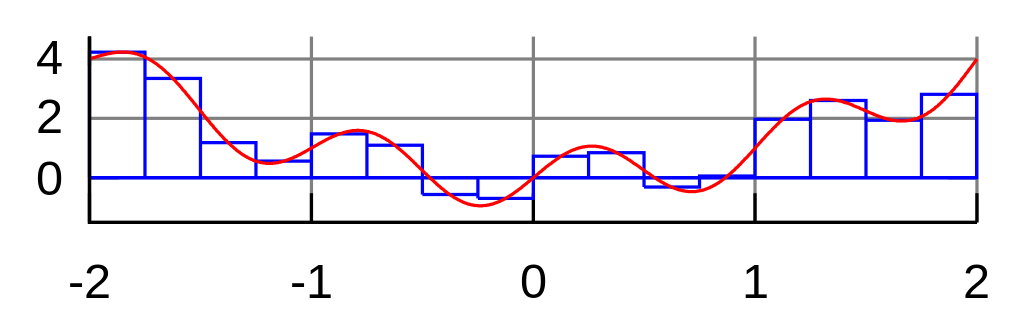
\includegraphics[width=1.0\textwidth]{figures/NumericalIntegration_rectangle}
      \end{center}
      \vspace{-22pt}
      \hspace*{15pt}\hbox{\thinspace{\tinytiny\itshape Wikipedia}}
  \end{columns}

  \vspace{15pt}
  \pause

  \begin{onlyenv}<1>
    \vspace{89pt}
  \end{onlyenv}

  \begin{onlyenv}<2-3>
  \begin{code}[linebackgroundcolor={
      }
    ]
double totalIntegral = 0;
for (int64_t i = 0; i < numberOfIntervals; ++i) {
  const double @orangex@orange =
    <@${\textcolor{darkred}{lower}}$@> + (i/numberOfIntervals) * (<@${\textcolor{blue}{upper}}$@> - <@${\textcolor{darkred}{lower}}$@>);
  const double thisIntervalsContribution = <@${\textcolor{darkgreen}{function}}$@>(@orangex@orange);
  totalIntegral += thisIntervalsContribution;
}
totalIntegral *= dx;
  \end{code}
  \end{onlyenv}

  \begin{onlyenv}<1-3>
    \vspace{10pt}
  \end{onlyenv}

  \begin{onlyenv}<4->
  \begin{code}[linebackgroundcolor={
        \btLstHL<4->{3-6}{bodyColor}
      }
    ]
double totalIntegral = 0;
@patternfor@pattern (int64_t @policyi = 0; i < numberOfIntervals; ++i@policy) {
  const double @orangex@orange =
    <@${\textcolor{darkred}{lower}}$@> + (i/numberOfIntervals) * (<@${\textcolor{blue}{upper}}$@> - <@${\textcolor{darkred}{lower}}$@>);
  const double thisIntervalsContribution = <@${\textcolor{darkgreen}{function}}$@>(@orangex@orange);
  totalIntegral += thisIntervalsContribution;
}
totalIntegral *= dx;
  \end{code}

  \begin{textblock*}{0.5\textwidth}(0.09\textwidth,0.45\textheight)
    \only<4->{\footnotesize {\color{orange!80} Pattern?}}
  \end{textblock*}

  \begin{textblock*}{0.5\textwidth}(0.76\textwidth,0.49\textheight)
    \only<4->{\footnotesize {\color{darkgreen!80} Policy?}}
  \end{textblock*}

  \begin{textblock*}{0.5\textwidth}(0.08\textwidth,0.585\textheight)
    \only<4->{\rotatebox{90}{\footnotesize {\color{blue!80} Body?}}}
  \end{textblock*}
  \pause
  \vspace{10pt}

  \end{onlyenv}

  \begin{onlyenv}<1-2>
    \vspace{10pt}
  \end{onlyenv}

  \begin{onlyenv}<3-4>
  How do we \textbf{parallelize} it?  \textit{Correctly?}
  \end{onlyenv}

\end{frame}

%==========================================================================

\begin{frame}[fragile]{Scalar integration (1)}

  \textbf{\ul{An (incorrect) attempt}}:

  \vspace{5pt}

  \begin{code}[linebackgroundcolor={
        \btLstHL<1->{4-6}{bodyColor}
      },
      frame=single
    ]
double totalIntegral = 0;
@patternKokkos::parallel_for@pattern(@policynumberOfIntervals@policy,
  [=] (const int64_t index) {
    const double x =
      lower + (index/numberOfIntervals) * (upper - lower);
    totalIntegral += function(x);}
  );
totalIntegral *= dx;
  \end{code}

\vspace{15pt}

{\color{red}First problem}: compiler error; cannot increment \texttt{totalIntegral} \\
  \hspace{20pt}(lambdas capture by value and are treated as const!)

\end{frame}

%==========================================================================

\begin{frame}[fragile]{Scalar integration (2)}

  \textbf{\ul{An (incorrect) solution to the (incorrect) attempt}}:

  \vspace{5pt}

  \begin{code}[linebackgroundcolor={
      },
      frame=single
    ]
@graydouble totalIntegral = 0;@gray
@darkreddouble * totalIntegralPointer = &totalIntegral;@darkred
@grayKokkos::parallel_for(numberOfIntervals,
  [=] (const int64_t index) {
    const double x =
      lower + (index/numberOfIntervals) * (upper - lower);@gray
    @darkred*totalIntegralPointer@darkred @gray+= function(x);}
  );
totalIntegral *= dx;@gray
  \end{code}

  \pause
  \vspace{5pt}

  {\color{red}Second problem}: race condition

  \vspace{-7pt}

  \begin{center}
  \begin{tabular}{| c | c | c |}
    \hline
    step & thread 0 & thread 1 \\
    \hline
    0 & load & \\
    \hline
    1 & increment & load \\
    \hline
    2 & write & increment \\
    \hline
    3 & & write \\
    \hline
  \end{tabular}
  \end{center}

  \vspace{-7pt}

\end{frame}

%==========================================================================

\begin{frame}[fragile]{Scalar integration (3)}

  {\color{red}Root problem}: we're using the \textbf{wrong pattern}, \emph{for} instead of \emph{reduction}

  \pause
  \vspace{5pt}

  \begin{block}{Important concept: Reduction}
    Reductions combine the results contributed by parallel work.
  \end{block}

  \vspace{10pt}
  \pause

  How would we do this with \textbf{OpenMP}?

  \vspace{-3pt}

  \begin{code}[linebackgroundcolor={
        \btLstHL<3->{4}{bodyColor}
      }
    ]
double finalReducedValue = 0;
#pragma @policyomp parallel@policy @patternfor reduction@pattern(@pattern+:finalReducedValue@pattern)
@patternfor@pattern (int64_t i = @policy0; i < N; ++i@policy) {
  finalReducedValue += ...
}
  \end{code}

  \pause
  How will we do this with \textbf{Kokkos}?

  \vspace{-3pt}

  \begin{code}[linebackgroundcolor={
        \btLstHL<4->{4}{bodyColor}
      }
    ]
double finalReducedValue = 0;
@patternparallel_reduce@pattern(@policyN@policy, @bodyfunctor@body, finalReducedValue);
  \end{code}

  \vspace{-5pt}

\end{frame}

%==========================================================================

\begin{frame}[fragile]{Scalar integration (4)}

  \ul{\textbf{Example: Scalar integration}}

  \vspace{5pt}

  \begin{code}[linebackgroundcolor={
        \btLstHL<1->{4}{bodyColor}
      },
      frame=single
    ]
double totalIntegral;
#pragma @policyomp parallel@policy @patternfor reduction@pattern(@pattern+:totalIntegral@pattern)
@patternfor@pattern (int64_t i = @policy0; i < numberOfIntervals; ++i@policy) {
  totalIntegral += function(...);
}
  \end{code}

  \begin{code}[linebackgroundcolor={
        \btLstHL<1->{4}{bodyColor}
      },
      frame=single
    ]
double totalIntegral = 0;
@patternparallel_reduce@pattern(@policynumberOfIntervals@policy,
  [=] (const int64_t i, double & valueToUpdate) {
    valueToUpdate += function(...);
  },
  totalIntegral);
  \end{code}

  \begin{textblock*}{0.5\textwidth}(0.05\textwidth,0.22\textheight)
    \rotatebox{90}{\textbf{OpenMP}}
  \end{textblock*}

  \begin{textblock*}{0.5\textwidth}(0.05\textwidth,0.49\textheight)
    \rotatebox{90}{\textbf{Kokkos}}
  \end{textblock*}

  \vspace{-5pt}

  \begin{itemize}
  \item The operator takes \textbf{two arguments}: a work index and a
  value to update.
  \item The second argument is a \textbf{thread-private value} that is
  managed by Kokkos; it is not the final reduced value.
    %by the way, that's what openmp is doing
  \end{itemize}

\end{frame}

%==========================================================================

\iffull
\begin{frame}[fragile]{Amdahl's Law (1)}

  \vspace{-10pt}
  \begin{alertblock}{Warning: Parallelism is NOT free}
    Dispatching (launching) parallel work has non-negligible cost.
  \end{alertblock}

  \pause

  {Simplistic data-parallel performance model: Time = $ \alpha + \frac{\beta * N}{P} $}
  \begin{itemize}
  \item {$\alpha$ = dispatch overhead}
  \item {$\beta$ = time for a unit of work}
  \item {$N$ = number of units of work}
  \item {$P$ = available concurrency}
  \end{itemize}

  \pause

  Speedup = {$P \div {\left( 1 + \frac{\alpha * P}{\beta * N} \right)}$}
  \begin{itemize}
  \item Should have {$\alpha * P \ll \beta * N$}
  \item \textit{All} runtimes strive to minimize launch overhead $\alpha$
  \item Find more parallelism to increase $N$
  \item Merge (fuse) parallel operations to increase $\beta$
  \end{itemize}

  \vspace{-10pt}

\end{frame}
\fi

%==========================================================================

\iffull
\begin{frame}[fragile]{Amdahl's Law (2)}

  \vspace{12pt}

  \textbf{\ul{Results}}:
  {illustrates simple speedup model = {$P \div {\left( 1 + \frac{\alpha * P}{\beta * N} \right)}$}}

  \vspace{-32pt}

  \begin{center}
    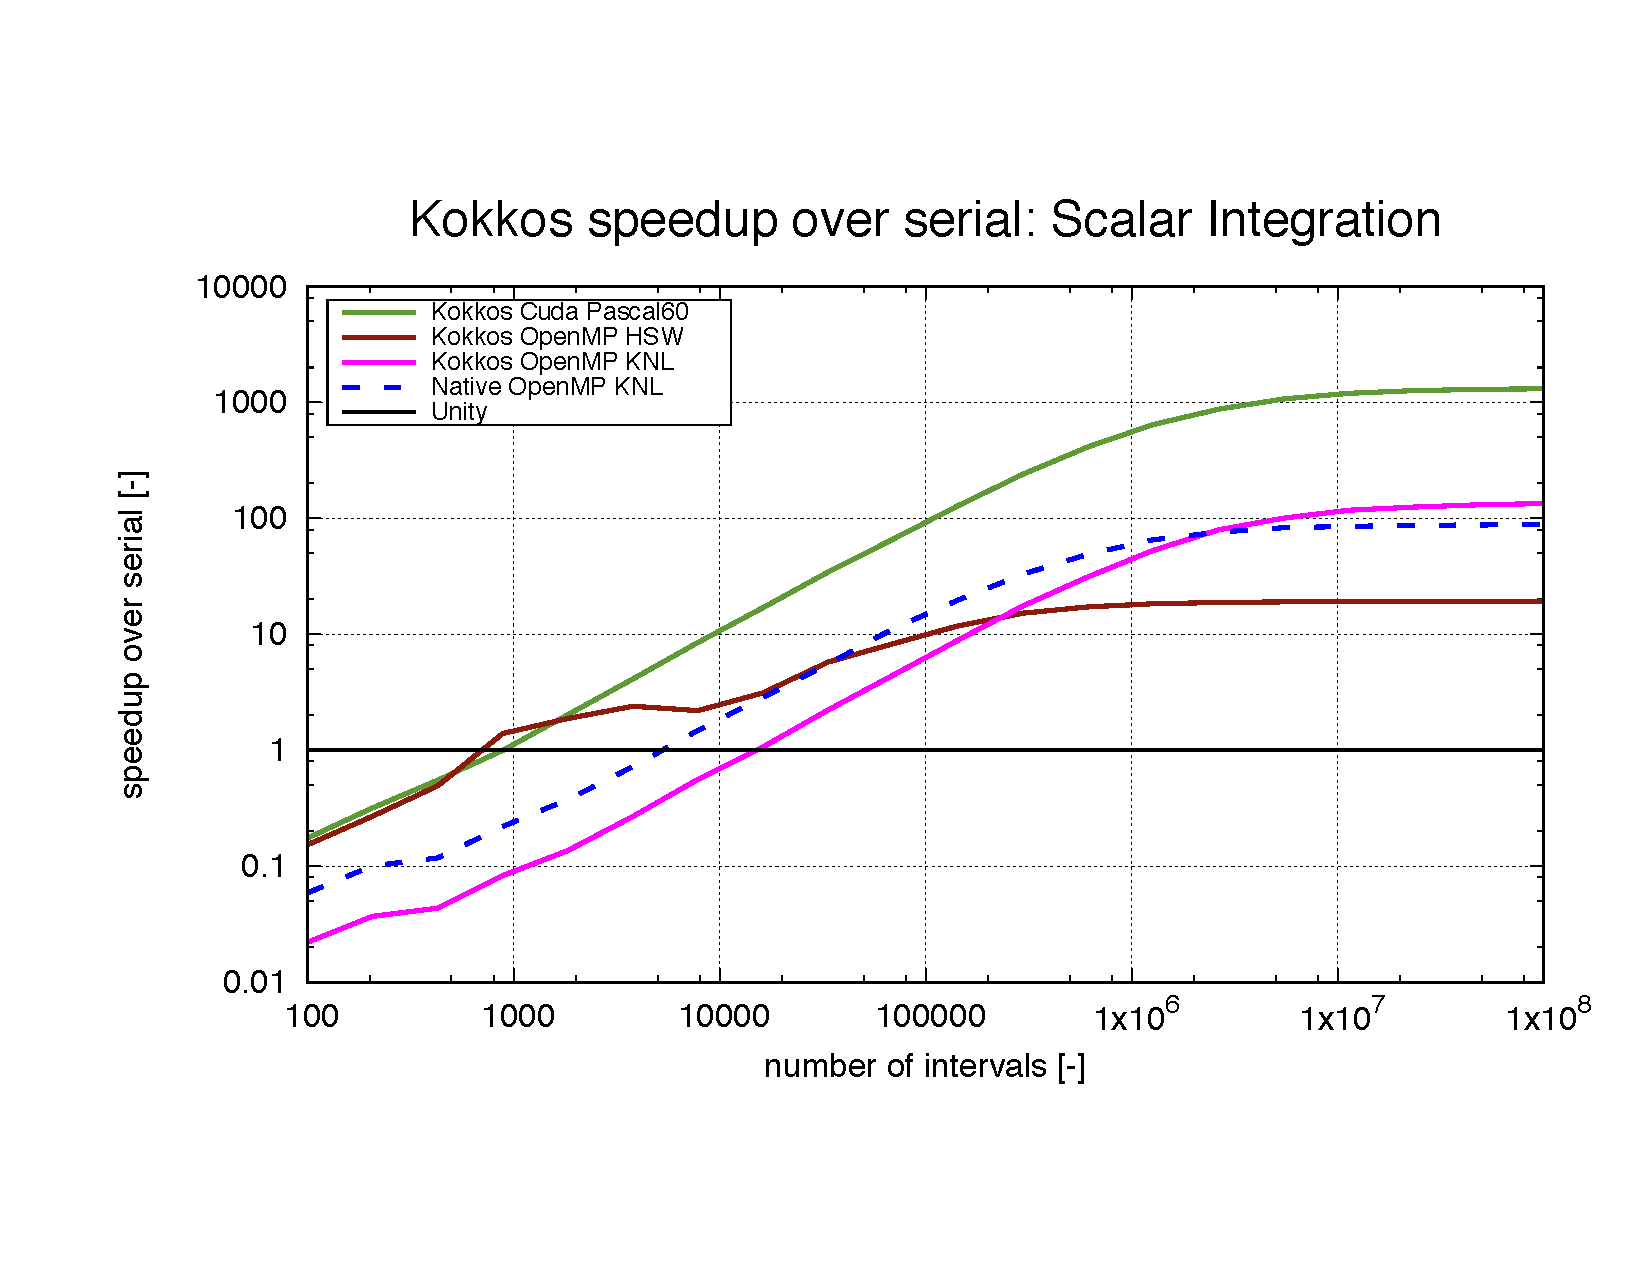
\includegraphics[width=1.00\textwidth]{figures/ScalarIntegration.pdf}
  \end{center}

  \vspace{-24pt}

  \begin{textblock*}{0.5\textwidth}(1.06\textwidth,0.33\textheight)
    \rotatebox{90}{\textbf{Note: log scale}}
  \end{textblock*}

\end{frame}
\fi

%==========================================================================

\begin{frame}[fragile]{Naming your kernels}
  \vspace{-10pt}
  \begin{alertblock}{Always name your kernels!}
     Giving unique names to each kernel is immensely helpful for debugging and profiling. You will regret it if you don't!
  \end{alertblock}
 
  \begin{itemize}
     \item Non-nested parallel patterns can take an optional string argument.
     \item The label doesn't need to be unique, but it is helpful.
     \item Anything convertible to "std::string"
     \item Used by profiling and debugging tools (see Profiling Tutorial)
  \end{itemize}
  \textbf{Example:} 
  \begin{code}[linebackgroundcolor={
        \btLstHL<1->{4}{bodyColor}
      },
      frame=single
    ]
double totalIntegral = 0;
@patternparallel_reduce@pattern("Reduction",@policynumberOfIntervals@policy,
  [=] (const int64_t i, double & valueToUpdate) {
    valueToUpdate += function(...);
  },
  totalIntegral);
  \end{code}
\end{frame}

%==========================================================================

\begin{frame}[fragile]{Recurring Exercise: Inner Product}

  \textbf{Exercise}: Inner product $<y, A * x>$

  \vspace{-10pt}

  \begin{center}
    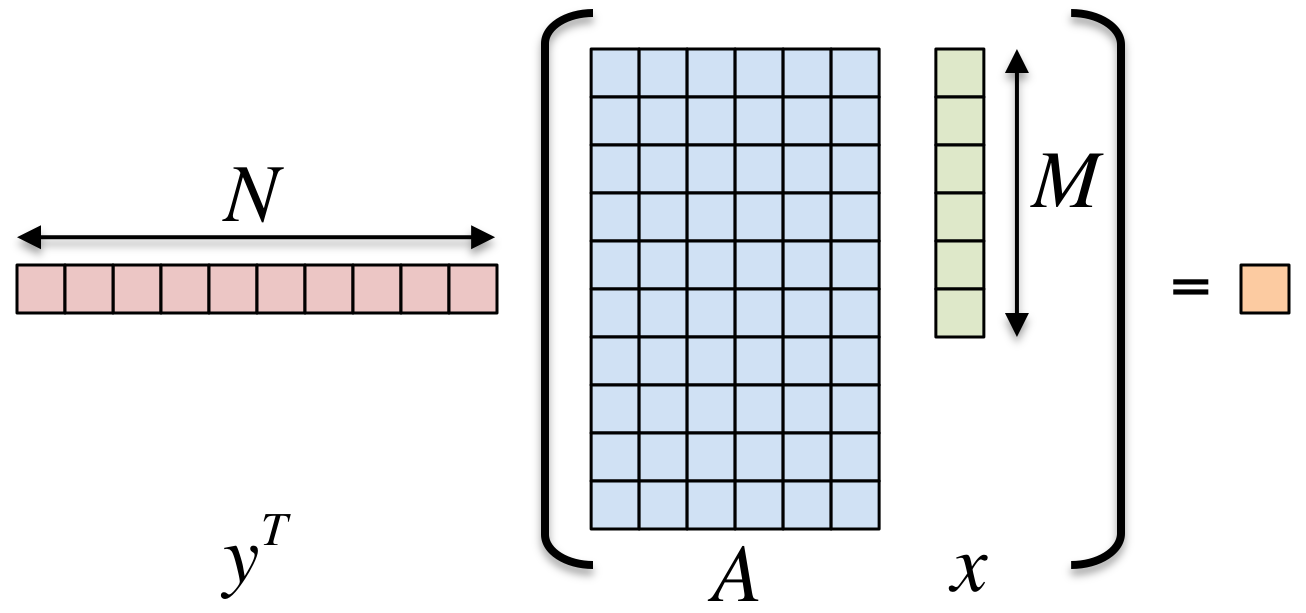
\includegraphics[width=0.80\textwidth]{figures/InnerProductExample_annotated}
  \end{center}

  \vspace{-15pt}

  \textbf{Details}:
  \begin{itemize}
    \item $y$ is $Nx1$, $A$ is $NxM$, $x$ is $Mx1$
    \item We'll use this exercise throughout the tutorial
  \end{itemize}

\end{frame}

%==========================================================================

\begin{frame}[fragile]{Exercise \#1: include, initialize, finalize Kokkos}

  The \textbf{first step} in using Kokkos is to include, initialize, and finalize:

  \begin{code}
#include <Kokkos_Core.hpp>
int main(int argc, char* argv[]) {
  /* ... do any necessary setup (e.g., initialize MPI) ... */
  Kokkos::initialize(argc, argv);
  {
  /* ... do computations ... */
  }
  Kokkos::finalize();
  return 0;
}
  \end{code}

  \vspace{7pt}

  (Optional) Command-line arguments or environment variables:

  \vspace{3pt}

	\begin{tabular}{| p{0.5\textwidth} | p{0.5\textwidth} |}
    \hline
	  \texttt{--kokkos-num-threads=INT} or \texttt{KOKKOS\_NUM\_THREADS} & total number of threads \\
    \hline
	  \texttt{--kokkos-device-id=INT} or \texttt{KOKKOS\_DEVICE\_ID} & device (GPU) ID to use \\
    \hline
  \end{tabular}

\end{frame}

%==========================================================================


\begin{frame}[fragile]{Exercise \#1: Inner Product, Flat Parallelism on the CPU}

  \vspace{5pt}

  \textbf{Exercise}: Inner product $<y, A * x>$

  \vspace{-10pt}

  \begin{center}
    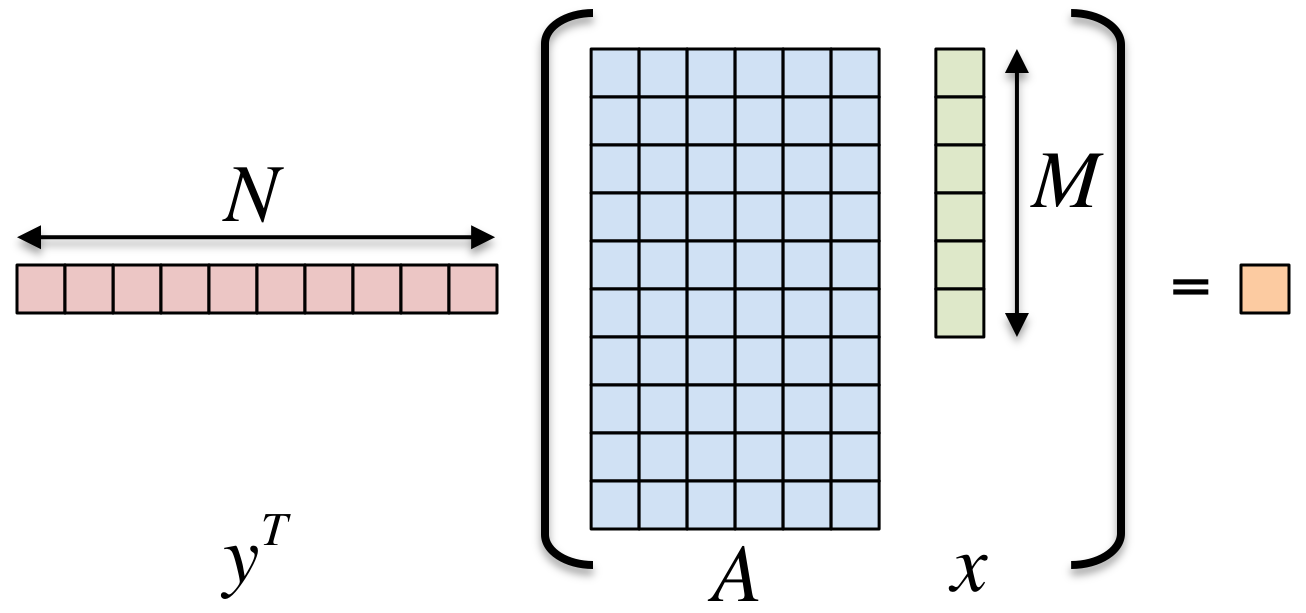
\includegraphics[width=0.65\textwidth]{figures/InnerProductExample_annotated}
  \end{center}

  \vspace{-30pt}

  \textbf{Details}:
  \begin{small}
  \begin{itemize}
\item Location: \ExerciseDirectory{01/Begin}
\item Look for comments labeled with ``EXERCISE''
\item Need to include, initialize, and finalize Kokkos library
\item Parallelize loops with \texttt{parallel\_for} or \texttt{parallel\_reduce}
\item Use lambdas instead of functors for computational bodies.
\item For now, this will only use the CPU.
\end{itemize}
  \end{small}

\end{frame}

%==========================================================================

\begin{frame}[fragile]{Exercise \#1: logistics}

\ul{\textbf{Compiling for CPU}}

\vspace{-3pt}
  \begin{small}
  \begin{code}
  cmake -B build_openmp -DKokkos_ENABLE_OPENMP=ON \
      -DCMAKE_BUILD_TYPE=Release
  cmake --build build_openmp
  \end{code}
  \end{small}

%  \hspace{10pt} {\tiny \url{https://github.com/kokkos/kokkos/wiki/Compiling#table-43-architecture-variables}}

\ul{\textbf{Running on CPU} with OpenMP backend}

\vspace{-3pt}
  \begin{small}
  \begin{code}
  # Set OpenMP affinity
  export OMP_NUM_THREADS=8
  export OMP_PROC_BIND=spread OMP_PLACES=threads
  # Print example command line options:
  ./build_openmp/01_Exercise -h
  # Run with defaults on CPU
  ./build_openmp/01_Exercise
  # Run larger problem
  ./build_openmp/01_Exercise -S 26
  \end{code}
  \end{small}

\ul{\textbf{Things to try:}}
  \begin{small}
  \begin{itemize}
  \itemsep0em
%  \item Vary number of threads
  \item Vary problem size with command line argument -S $s$
  \item Vary number of rows with command line argument -N $n$
  \item Num rows = $2^n$, num cols = $2^m$, total size = $2^s == 2^{n+m}$
  \end{itemize}
  \end{small}
\end{frame}

%==========================================================================

\begin{frame}[fragile]{Exercise \#1 results}

  \vspace{-10pt}

  \begin{center}
    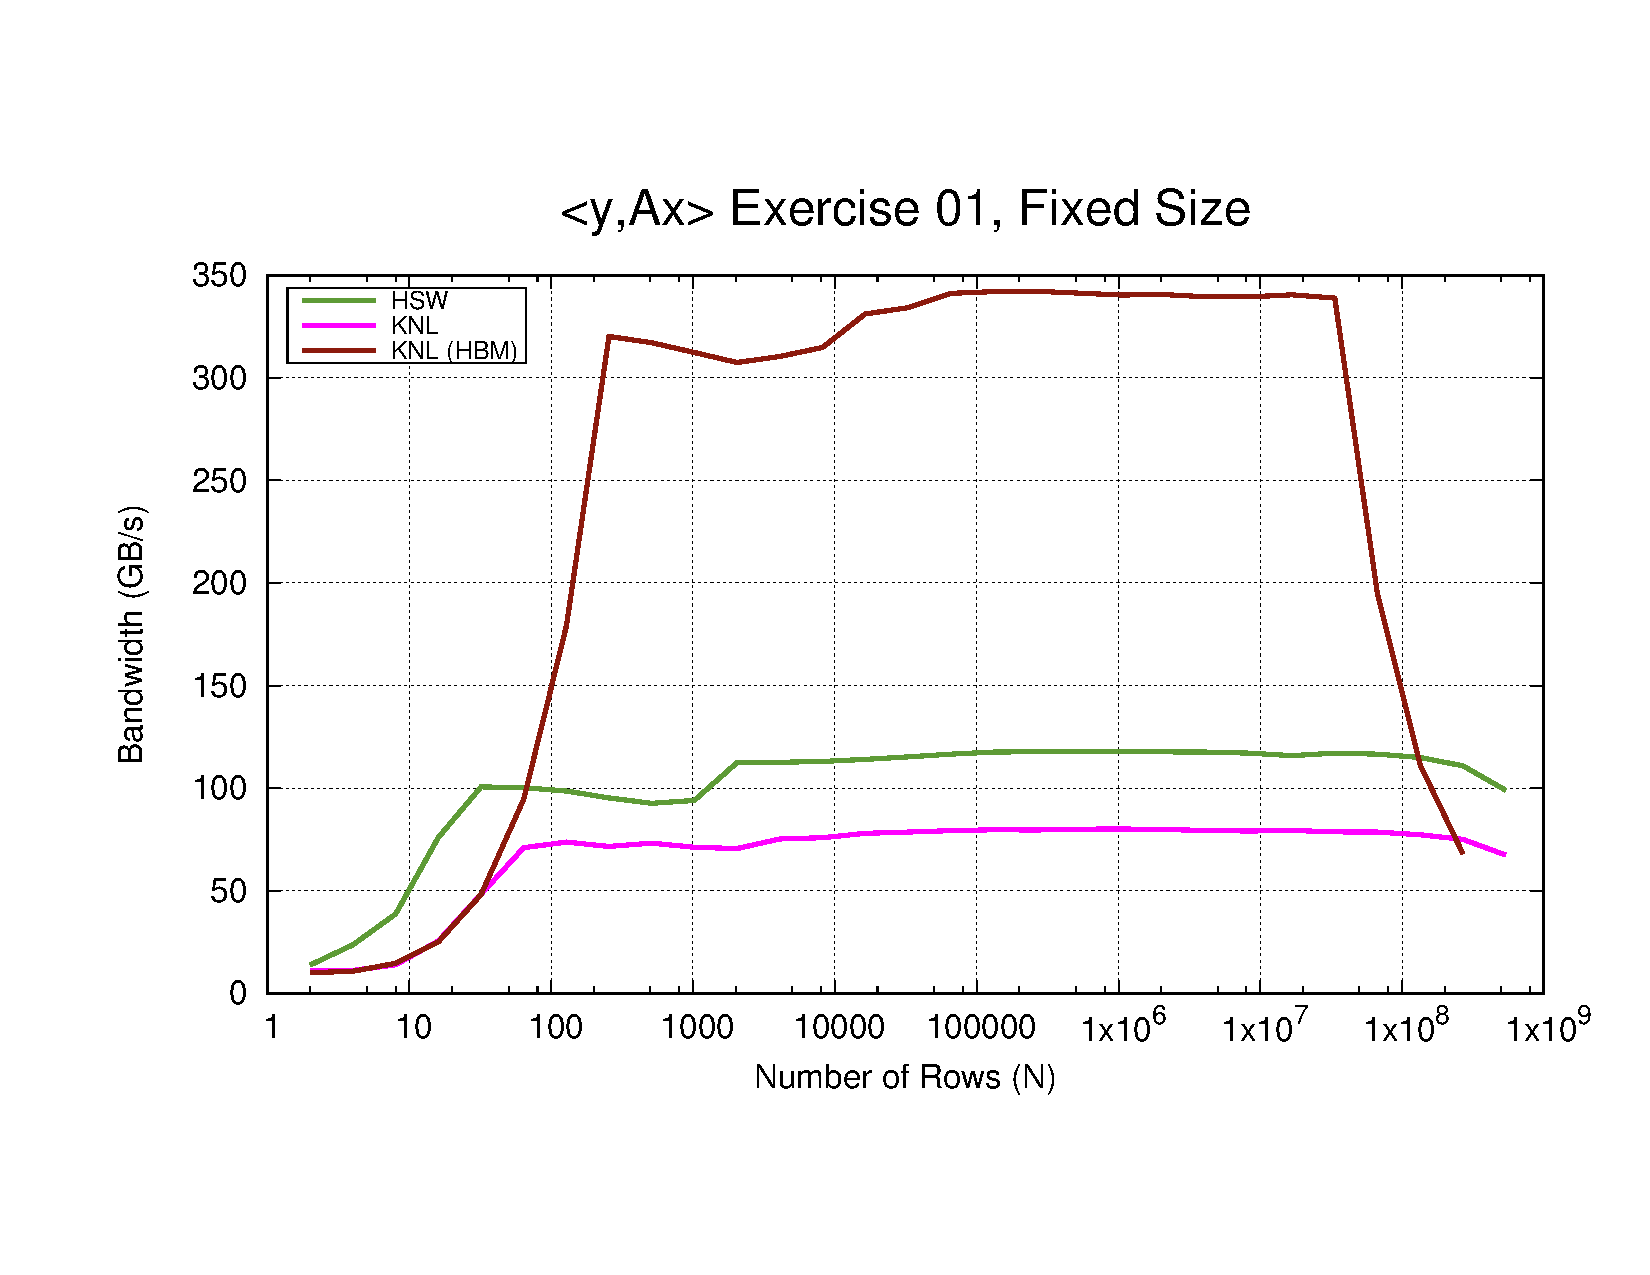
\includegraphics[viewport=1.25in 3.0in 10in 6in, width=1.0\textwidth]{figures/Exercise01-Performance.pdf}
  \end{center}

  \vspace{-15pt}

\end{frame}

%==========================================================================

\iffull
\begin{frame}[fragile]{Exercise \#1 Going beyond}
   \ul{\textbf{More things to try: port your solution to work on the device}}
   \begin{itemize}
     \item You will need to update the dynamic memory allocation.
     \item Replace \texttt{std::malloc} and \texttt{std::free} with \texttt{Kokkos::kokkos\_malloc} and \texttt{Kokkos::kokkos\_free}.
     \item Bonus question:  Why does this perform so poorly?  (hint: the answer is in this slide deck somewhere)
     \item Note that this is just for learning purposes and by no mean a recommended way to manage the lifetime of your arrays.  We will see a better way to do this soon.
   \end{itemize}

   \ul{\textbf{Compiling for GPU}}
  \vspace{-3pt}
  \begin{small}
  \begin{code}
  # if the architecture autodetection fails configure with
  # -DKokkos_ARCH_VOLTA70=ON for V100
  # refer to the documentation for the complete list of supported NVIDIA GPU
  # architectures and corresponding flags, or use ccmake to discover options
    cmake -B build-cuda -DKokkos_ENABLE_CUDA=ON
    cmake --build build-cuda
    make -j KOKKOS_DEVICES=Cuda KOKKOS_ARCH=...
  \end{code}
  \end{small}
\end{frame}
\fi

%==========================================================================

\iffull
\begin{frame}[fragile]{Basic capabilities we haven't covered}

  \begin{itemize}

  \item {Customizing \texttt{parallel\_reduce} data type and reduction operator
    \\ \hspace{10pt} \emph{e.g.}, minimum, maximum, ...}

  \item {\texttt{parallel\_scan} pattern for exclusive and inclusive prefix sum}

  \item {Using \textit{tag dispatch} interface to allow non-trivial functors to have multiple ``\texttt{operator()}'' functions.
    \\ \hspace{10pt} very useful in large, complex applications}

  \end{itemize}

\end{frame}
\fi

%==========================================================================

\begin{frame}{Section Summary}

  \begin{itemize}
    \item{\textbf{Simple} usage is similar to OpenMP, advanced features are also straightforward}
    \item{Three common \textbf{data-parallel patterns} are \texttt{parallel\_for}, \texttt{parallel\_reduce}, and \texttt{parallel\_scan}.}
    \item{A parallel computation is characterized by its \textbf{pattern}, \textbf{policy}, and \textbf{body}.}
    \item{User provides \textbf{computational bodies} as functors or lambdas which handle a single work item.}
  \end{itemize}

\end{frame}


%==========================================================================

\begin{frame}[fragile]

  {\Huge Views}

  \vspace{20pt}

  \textbf{Learning objectives:}
  \begin{itemize}
    \item{Motivation behind the \texttt{View} abstraction.}
    \item{Key \texttt{View} concepts and template parameters.}
    \item{The \texttt{View} life cycle.}
  \end{itemize}

  \vspace{-20pt}

\end{frame}

%==========================================================================

\begin{frame}[fragile]{View motivation}

  \textbf{\ul{Example: running \texttt{daxpy} on the GPU:}}

  \vspace{5pt}

  \begin{code}[linebackgroundcolor={
        \btLstHL<2->{3}{red!30}
      },
      frame=single
    ]
double * x = new double[N]; // also y
parallel_for("DAXPY",N, [=] (const int64_t i) {
    y[i] = a * x[i] + y[i];
  });
  \end{code}

  \begin{code}[linebackgroundcolor={
        \btLstHL<2->{2,4}{red!30}
      },
      frame=single
    ]
struct Functor {
  double *_x, *_y, a;
  void operator()(const int64_t i) const {
    _y[i] = _a * _x[i] + _y[i];
  }
};
  \end{code}

  \begin{textblock*}{0.5\textwidth}(0.05\textwidth,0.225\textheight)
    \rotatebox{90}{\textbf{Lambda}}
  \end{textblock*}

  \begin{textblock*}{0.5\textwidth}(0.05\textwidth,0.470\textheight)
    \rotatebox{90}{\textbf{Functor}}
  \end{textblock*}

  \vspace{5pt}
  \pause

  \textbf{{\color{red}Problem}}: \texttt{x} and \texttt{y} reside in CPU memory.

  \vspace{5pt}
  \pause

  \textbf{Solution:} We need a way of storing data (multidimensional arrays) which can be communicated to an accelerator (GPU).

  \vspace{5pt}

  \hspace{20pt}{\Large $\Rightarrow$ \textbf{Views}}

  \vspace{-5pt}

\end{frame}

%==========================================================================

\begin{frame}[fragile]{Views (0)}

  \ul{\textbf{View} abstraction}
  \begin{itemize}
  \item {A \textit{lightweight} C++ class with a pointer to array data and a little meta-data,}
  \item {that is \textit{templated} on the data type (and other things).}
  \end{itemize}

  \vspace{5pt}

  \ul{\textbf{High-level example} of Views for \texttt{daxpy} using lambda}:

  \begin{code}[frame=single, keywords={}]
@blueView<double*, ...>@blue x(...), y(...);
@gray...populate x, y... @gray

parallel_for("DAXPY",N, [=] (const int64_t i) {
    // Views x and y are captured by value (shallow copy)
    y(i) = a * x(i) + y(i);
  });
  \end{code}

  \pause
  \vspace{0pt}

  \begin{block}{Important point}
    Views are \textbf{like pointers}, so copy them in your functors.
  \end{block}

  \vspace{5pt}

\end{frame}

%==========================================================================

\begin{frame}[fragile]{Views (1)}

  \ul{\textbf{View} overview:}

  \begin{itemize}
    \item{\textbf{Multi-dimensional array} of 0 or more dimensions \\
          \hspace{20pt}scalar (0), vector (1), matrix (2), etc.}
    \item{\textbf{Number of dimensions (rank)} is fixed at compile-time.}
    \item{Arrays are \textbf{rectangular}, not ragged.}
    \item{\textbf{Sizes of dimensions} set at compile-time or runtime. \\
          \hspace{20pt}e.g., 2x20, 50x50, etc.}
    \item{Access elements via "(...)" operator.}
  \end{itemize}

  \pause
  \vspace{-3pt}

  \textbf{Example}:
  \vspace{-3pt}
  \begin{code}[keywords={double,View}]
View<double***> data("label", N0, N1, N2); //<@3 run, 0 compile@>
View<double**[N2]> data("label", N0, N1);  //<@2 run, 1 compile@>
View<double*[N1][N2]> data("label", N0);   //<@1 run, 2 compile@>
View<double[N0][N1][N2]> data("label");    //<@0 run, 3 compile@>
//Access
data(i,j,k) = 5.3;
  \end{code}

  \vspace{-1pt}
  Note: runtime-sized dimensions must come first.

\end{frame}

%==========================================================================

\begin{frame}[fragile]{Views (2)}

  \ul{\textbf{View} life cycle:}

  \begin{itemize}
    \item{Allocations only happen when \emph{explicitly} specified. \\
          \hspace{20pt}i.e., there are \textbf{no hidden allocations}.}
    \item{Copy construction and assignment are \textbf{shallow} (like pointers).\\
          \hspace{20pt}so, you pass \texttt{Views} by value, \emph{not} by reference}
    \item{Reference counting is used for \textbf{automatic deallocation.}}
    \item{They behave like \texttt{std::shared\_ptr}}
  \end{itemize}

  \pause
  \textbf{Example}:

  \vspace{-3pt}

  \begin{code}[keywords={}]
View<double*[5]> @bluea@blue("a", N), @darkgreenb@darkgreen("b", K);
@bluea@blue = @darkgreenb@darkgreen;
View<double**> @darkredc@darkred(@darkgreenb@darkgreen);
@bluea@blue(0,2) = 1;
@darkgreenb@darkgreen(0,2) = 2;
@darkredc@darkred(0,2) = 3;
print_value( @bluea@blue(0,2) );
  \end{code}

  \begin{textblock*}{0.5\textwidth}(0.6\textwidth,0.78\textheight)
    \onslide<2->{What gets printed?}
  \end{textblock*}

  \begin{textblock*}{0.5\textwidth}(0.65\textwidth,0.83\textheight)
    \onslide<3->{\texttt{3.0}}
  \end{textblock*}

\end{frame}

%==========================================================================

\begin{frame}[fragile]{Views (3)}

  \ul{\textbf{View} Properties:}

  \begin{itemize}
    \item Accessing a \texttt{View}'s sizes is done via its \texttt{extent(dim)} function.
         \begin{itemize}
		 \item Static extents can \emph{additionally} be accessed via \texttt{static\_extent(dim)}.
	 \end{itemize}
    \item You can retrieve a raw pointer via its \texttt{data()} function.
    \item The label can be accessed via \texttt{label()}.
  \end{itemize}

  \textbf{Example}:

  \begin{code}[keywords={View,extent,static_extent,data,label}]
	  View<double*[5]> a("A",N0);
	  assert(a.extent(0) == N0);
	  assert(a.extent(1) == 5);
	  static_assert(a.static_extent(1) == 5);
	  assert(a.data() != nullptr);
	  assert(a.label() == "A");
  \end{code}

\end{frame}
%==========================================================================

\begin{frame}[fragile]{Exercise \#2: Inner Product, Flat Parallelism on the CPU, with Views}

  \begin{small}
  \begin{itemize}
  \item Location: \ExerciseDirectory{02/Begin}
  \item Assignment: Change data storage from arrays to Views.
  \item Compile and run on CPU, and then on GPU with SharedSpace.
  \end{itemize}
  \end{small}

\begin{code}
# CPU-only using OpenMP
cmake -B build_openmp -DKokkos_ENABLE_OPENMP=ON
cmake --build build_openmp
# Run exercise
./build_openmp/02_Exercise -S 26
# Note the warnings, set appropriate environment variables
\end{code}

  \begin{scriptsize}
  \begin{itemize}
  \item Vary problem size: \textbf{-S \#}
  \item Vary number of rows: \textbf{-N \#}
  \item Vary repeats: \textbf{-nrepeat \#}
  \item Compare performance of CPU vs GPU
  \end{itemize}
  \end{scriptsize}

\end{frame}

%==========================================================================

\iffull
\begin{frame}[fragile]{Advanced features we haven't covered}

  \begin{itemize}

  \item {\textbf{Memory space} in which view's data resides;
         \textit{covered next}.}

  \item {\textbf{deep\_copy} view's data; \textit{covered later}. \\
        Note: Kokkos \textit{never} hides a deep\_copy of data.}

  \item {\textbf{Layout} of multidimensional array; \textit{covered later}.}

  \item {\textbf{Memory traits}; \textit{covered later}.}

  \item {\textbf{Subview}: Generating a view that is a ``slice'' of other multidimensional array view; \textit{covered later}.}

  \end{itemize}

\end{frame}
\fi



\ifmedium
\begin{frame}[fragile]{Execution and Memory spaces}

  {\Huge Execution and Memory Spaces}

  \vspace{20pt}

  \textbf{Learning objectives:}
  \begin{itemize}
    \item{Heterogeneous nodes and the \textbf{space} abstractions.}
    \item{How to control where parallel bodies are run, \textbf{execution space}.}
    \item{How to control where view data resides, \textbf{memory space}.}
    \item{How to avoid illegal memory accesses and manage data movement.}
    \item{The need for \texttt{Kokkos::initialize} and \texttt{finalize}.}
    \item{Where to use Kokkos annotation macros for portability.}
  \end{itemize}

  \vspace{-20pt}

\end{frame}
\fi

%==========================================================================

%\begin{frame}[fragile]{Execution spaces (0)}
%
%  \textbf{Thought experiment}: Consider this code:
%
%  \vspace{5pt}
%
%  \lstset{mathescape, escapeinside={<@}{@>},
%          language=C,
%          keywords={}}
%
%  \begin{lstlisting}[linebackgroundcolor={
%        \btLstHL{1-3}{darkred!20}
%      }
%    ]
%  MPI_Reduce(...);
%  FILE * file = fopen(...);
%  runANormalFunction(...data...);
%  \end{lstlisting}
%
%  \vspace{-11pt}
%
%  \begin{lstlisting}[linebackgroundcolor={
%        \btLstHL{3-4}{bodyColor}
%      }
%    ]
%  Kokkos::parallel_for(numberOfSomethings,
%                       [=] (const int64_t somethingIndex) {
%                         const double y = ...;
%                         // do something interesting
%                       }
%                       );
%  \end{lstlisting}
%
%  \begin{textblock*}{0.5\textwidth}(0.08\textwidth,0.235\textheight)
%    \rotatebox{90}{{\footnotesize {\color{darkred!80} section 1}}}
%  \end{textblock*}
%
%  \begin{textblock*}{0.5\textwidth}(0.08\textwidth,0.40\textheight)
%    \rotatebox{90}{{\footnotesize {\color{blue!80} section 2}}}
%  \end{textblock*}
%
%  \pause
%
%  \begin{itemize}
%    \item{Where will {\color{darkred!80}section 1} be run?  CPU?  GPU?}
%    \item{Where will {\color{blue!80}section 2} be run?  CPU?  GPU?}
%    \item{How do I \textbf{control} where code is executed?}
%  \end{itemize}
%
%  \pause
%  \vspace{5pt}
%
%  \hspace{20pt}{\Large $\Rightarrow$ \textbf{Execution spaces}}
%
%\end{frame}

%==========================================================================

\begin{frame}{Execution spaces (1)}

  \vspace{-15pt}

  \begin{center}
  \textbf{Execution Space} \\
  a homogeneous set of cores and an execution mechanism \\
  (i.e., ``place to run code'')
  \end{center}

  \vspace{-15pt}

  \begin{center}
    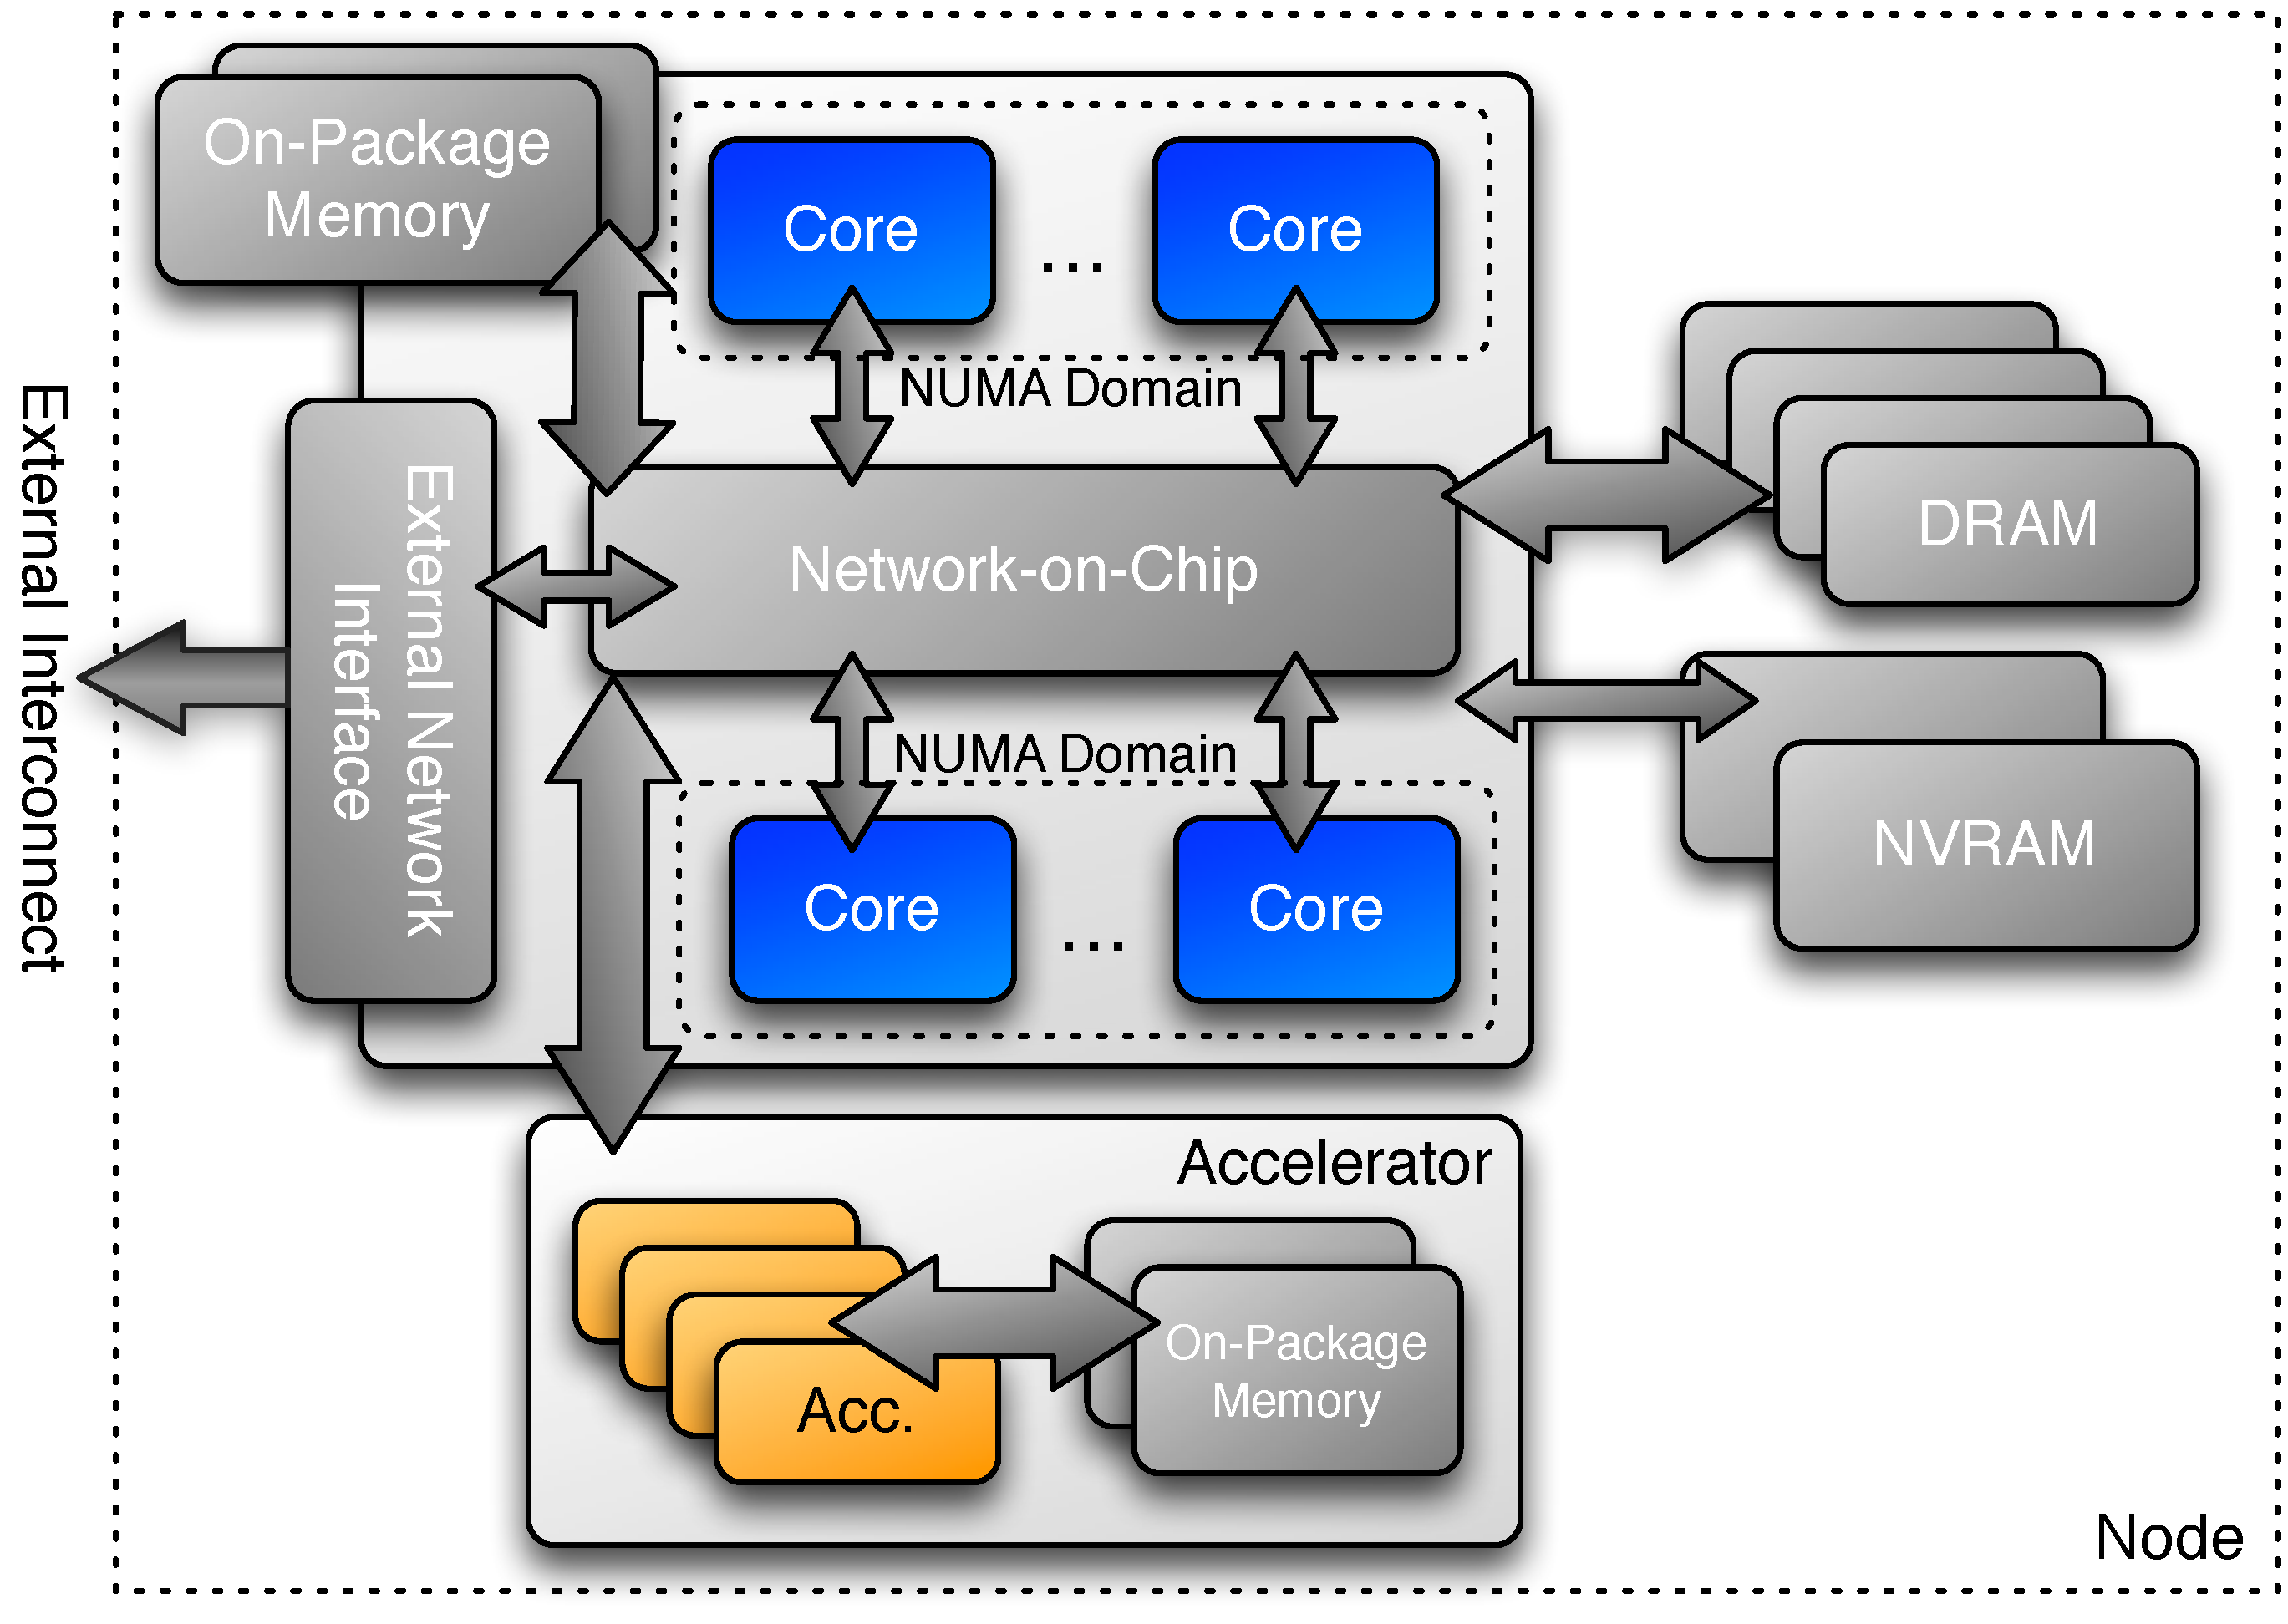
\includegraphics[width=0.70\textwidth]{figures/kokkos-execution-space}
  \end{center}

  \vspace{-12pt}

  {Execution spaces: \texttt{Serial, Threads, OpenMP, Cuda, HIP,} ... }

\end{frame}

%==========================================================================

\ifmedium
\begin{frame}[fragile]{Execution spaces (2)}

  \lstset{mathescape, escapeinside={<@}{@>},
          language=C,
          keywords={}}

  \begin{lstlisting}[linebackgroundcolor={
        \btLstHL{1-3}{darkred!20}
      }
    ]
  MPI_Reduce(...);
  FILE * file = fopen(...);
  runANormalFunction(...data...);
  \end{lstlisting}

  \vspace{-11pt}

  \begin{lstlisting}[linebackgroundcolor={
        \btLstHL{3-4}{bodyColor}
      }
    ]
  Kokkos::parallel_for("MyKernel", numberOfSomethings,
                       [=] (const int64_t somethingIndex) {
                         const double y = ...;
                         // do something interesting
                       }
                       );
  \end{lstlisting}

  \vspace{-5pt}

  \begin{textblock*}{0.5\textwidth}(0.08\textwidth,0.19\textheight)
    \rotatebox{90}{{\footnotesize {\color{darkred!80} Host}}}
  \end{textblock*}

  \begin{textblock*}{0.5\textwidth}(0.08\textwidth,0.315\textheight)
    \rotatebox{90}{{\footnotesize {\color{blue!80} Parallel}}}
  \end{textblock*}

  \pause

  \begin{itemize}
    \item<2->{Where will {\color{darkred!80}Host} code be run?  CPU?  GPU? \\
        \hspace{20pt}{$\Rightarrow$} Always in the \textbf{host process} \\
        \hspace{20pt} also known as \textbf{default host execution space}}
    \item<3->{Where will {\color{blue!80}Parallel} code be run?  CPU?  GPU? \\
      \hspace{20pt}{$\Rightarrow$} The \textbf{default execution space}}
    \item<4->{How do I \textbf{control} where the {\color{blue!80}Parallel} body is executed? \\
      \hspace{20pt}Changing the default execution space (\textit{at compilation}), \\
      \hspace{20pt}or specifying an execution space in the \textbf{policy}.}
  \end{itemize}

\end{frame}
\fi

%==========================================================================

\begin{frame}[fragile]{Execution spaces (3)}

  \textbf{\ul{Changing the parallel execution space:}}

  \vspace{3pt}

  \begin{code}[linebackgroundcolor={
        \btLstHL<1->{4}{bodyColor}
      },
      frame=single
    ]
@patternparallel_for@pattern("Label",
  @policyRangePolicy< @boldExecutionSpace@bold >(0,numberOfIntervals)@policy,
  [=] (const int64_t i) {
    /* ... body ... */
  });
  \end{code}

  \begin{code}[linebackgroundcolor={
        \btLstHL<1->{4}{bodyColor}
      },
      frame=single
    ]
@patternparallel_for@pattern("Label",
  @policynumberOfIntervals@policy, // => RangePolicy<>(0,numberOfIntervals)
  [=] (const int64_t i) {
    /* ... body ... */
  });
  \end{code}

  \begin{textblock*}{0.5\textwidth}(0.05\textwidth,0.465\textheight)
    \rotatebox{90}{\textbf{Default}}
  \end{textblock*}

  \begin{textblock*}{0.5\textwidth}(0.05\textwidth,0.23\textheight)
    \rotatebox{90}{\textbf{Custom}}
  \end{textblock*}

  \pause

  Requirements for enabling execution spaces:
  \vspace{-3pt}
  \begin{itemize}
    \item{Kokkos must be \textbf{compiled} with the execution spaces enabled.}
    \item{Execution spaces must be \textbf{initialized} (and \textbf{finalized}).}
    \item{\textbf{Functions} must be marked with a \textbf{macro} for non-CPU spaces.}
    \item{\textbf{Lambdas} must be marked with a \textbf{macro} for non-CPU spaces.}
  \end{itemize}

\end{frame}

%==========================================================================

\begin{frame}[fragile]{Execution spaces (5)}

  \textbf{\ul{Kokkos function and lambda portability annotation macros:}}

  \vspace{4pt}

  {Function annotation with \texttt{\footnotesize KOKKOS\_INLINE\_FUNCTION} macro}

  \begin{code}[keywords={}, frame=single, basicstyle=\tiny\ttfamily]
@graystruct ParallelFunctor {@gray
  KOKKOS_INLINE_FUNCTION
  @graydouble helperFunction(const int64_t s) const {...}@gray
  KOKKOS_INLINE_FUNCTION
  @grayvoid operator()(const int64_t index) const {
    helperFunction(index);
  }
}@gray
// Where kokkos defines:
#define KOKKOS_INLINE_FUNCTION inline                     // if CPU only
#define KOKKOS_INLINE_FUNCTION inline __device__ __host__ // if CPU + Cuda/HIP
  \end{code}

  \pause

  {Lambda annotation with \texttt{\footnotesize KOKKOS\_LAMBDA} macro}

  \begin{code}[keywords={}, frame=single, basicstyle=\tiny\ttfamily]
@grayKokkos::parallel_for("Label",numberOfIterations, @gray
  KOKKOS_LAMBDA@gray (const int64_t index) {...});@gray

// Where Kokkos defines:
#define KOKKOS_LAMBDA [=]                     // if CPU only
#define KOKKOS_LAMBDA [=] __device__ __host__ // if CPU + Cuda/HIP
  \end{code}

  These macros are \emph{already} defined by Kokkos.

  \vspace{-10pt}

\end{frame}

%==========================================================================

\ifmedium
\begin{frame}[fragile]{Memory Space Motivation}

  \ul{\textbf{Memory space motivating example:} summing an array}

  \begin{code}[linebackgroundcolor={
        \btLstHL<3-4>{3,10}{red!20}
      },
      keywords={}]
View<double*> data("data", size);
for (int64_t i = 0; i < size; ++i) {
  data(i) = ...read from file...
}

double sum = 0;
Kokkos::parallel_reduce("Label",
  RangePolicy<SomeExampleExecutionSpace>(0, size),
  KOKKOS_LAMBDA (const int64_t index, double & valueToUpdate) {
    valueToUpdate += data(index);
  },
  sum);
  \end{code}

  \pause
  \vspace{10pt}

  Question: Where is the data stored? GPU memory?  CPU memory?  Both?

  \pause
  \pause
  \vspace{10pt}

  \hspace{20pt}{\Large $\Rightarrow$ \textbf{Memory Spaces}}

\end{frame}
\fi

%==========================================================================

\begin{frame}[fragile]{Memory spaces (0)}

  \begin{center}
  \textbf{Memory space}: \\
     explicitly-manageable memory resource  \\
     (i.e., ``place to put data'')
  \end{center}

  \vspace{-20pt}

  \begin{center}
    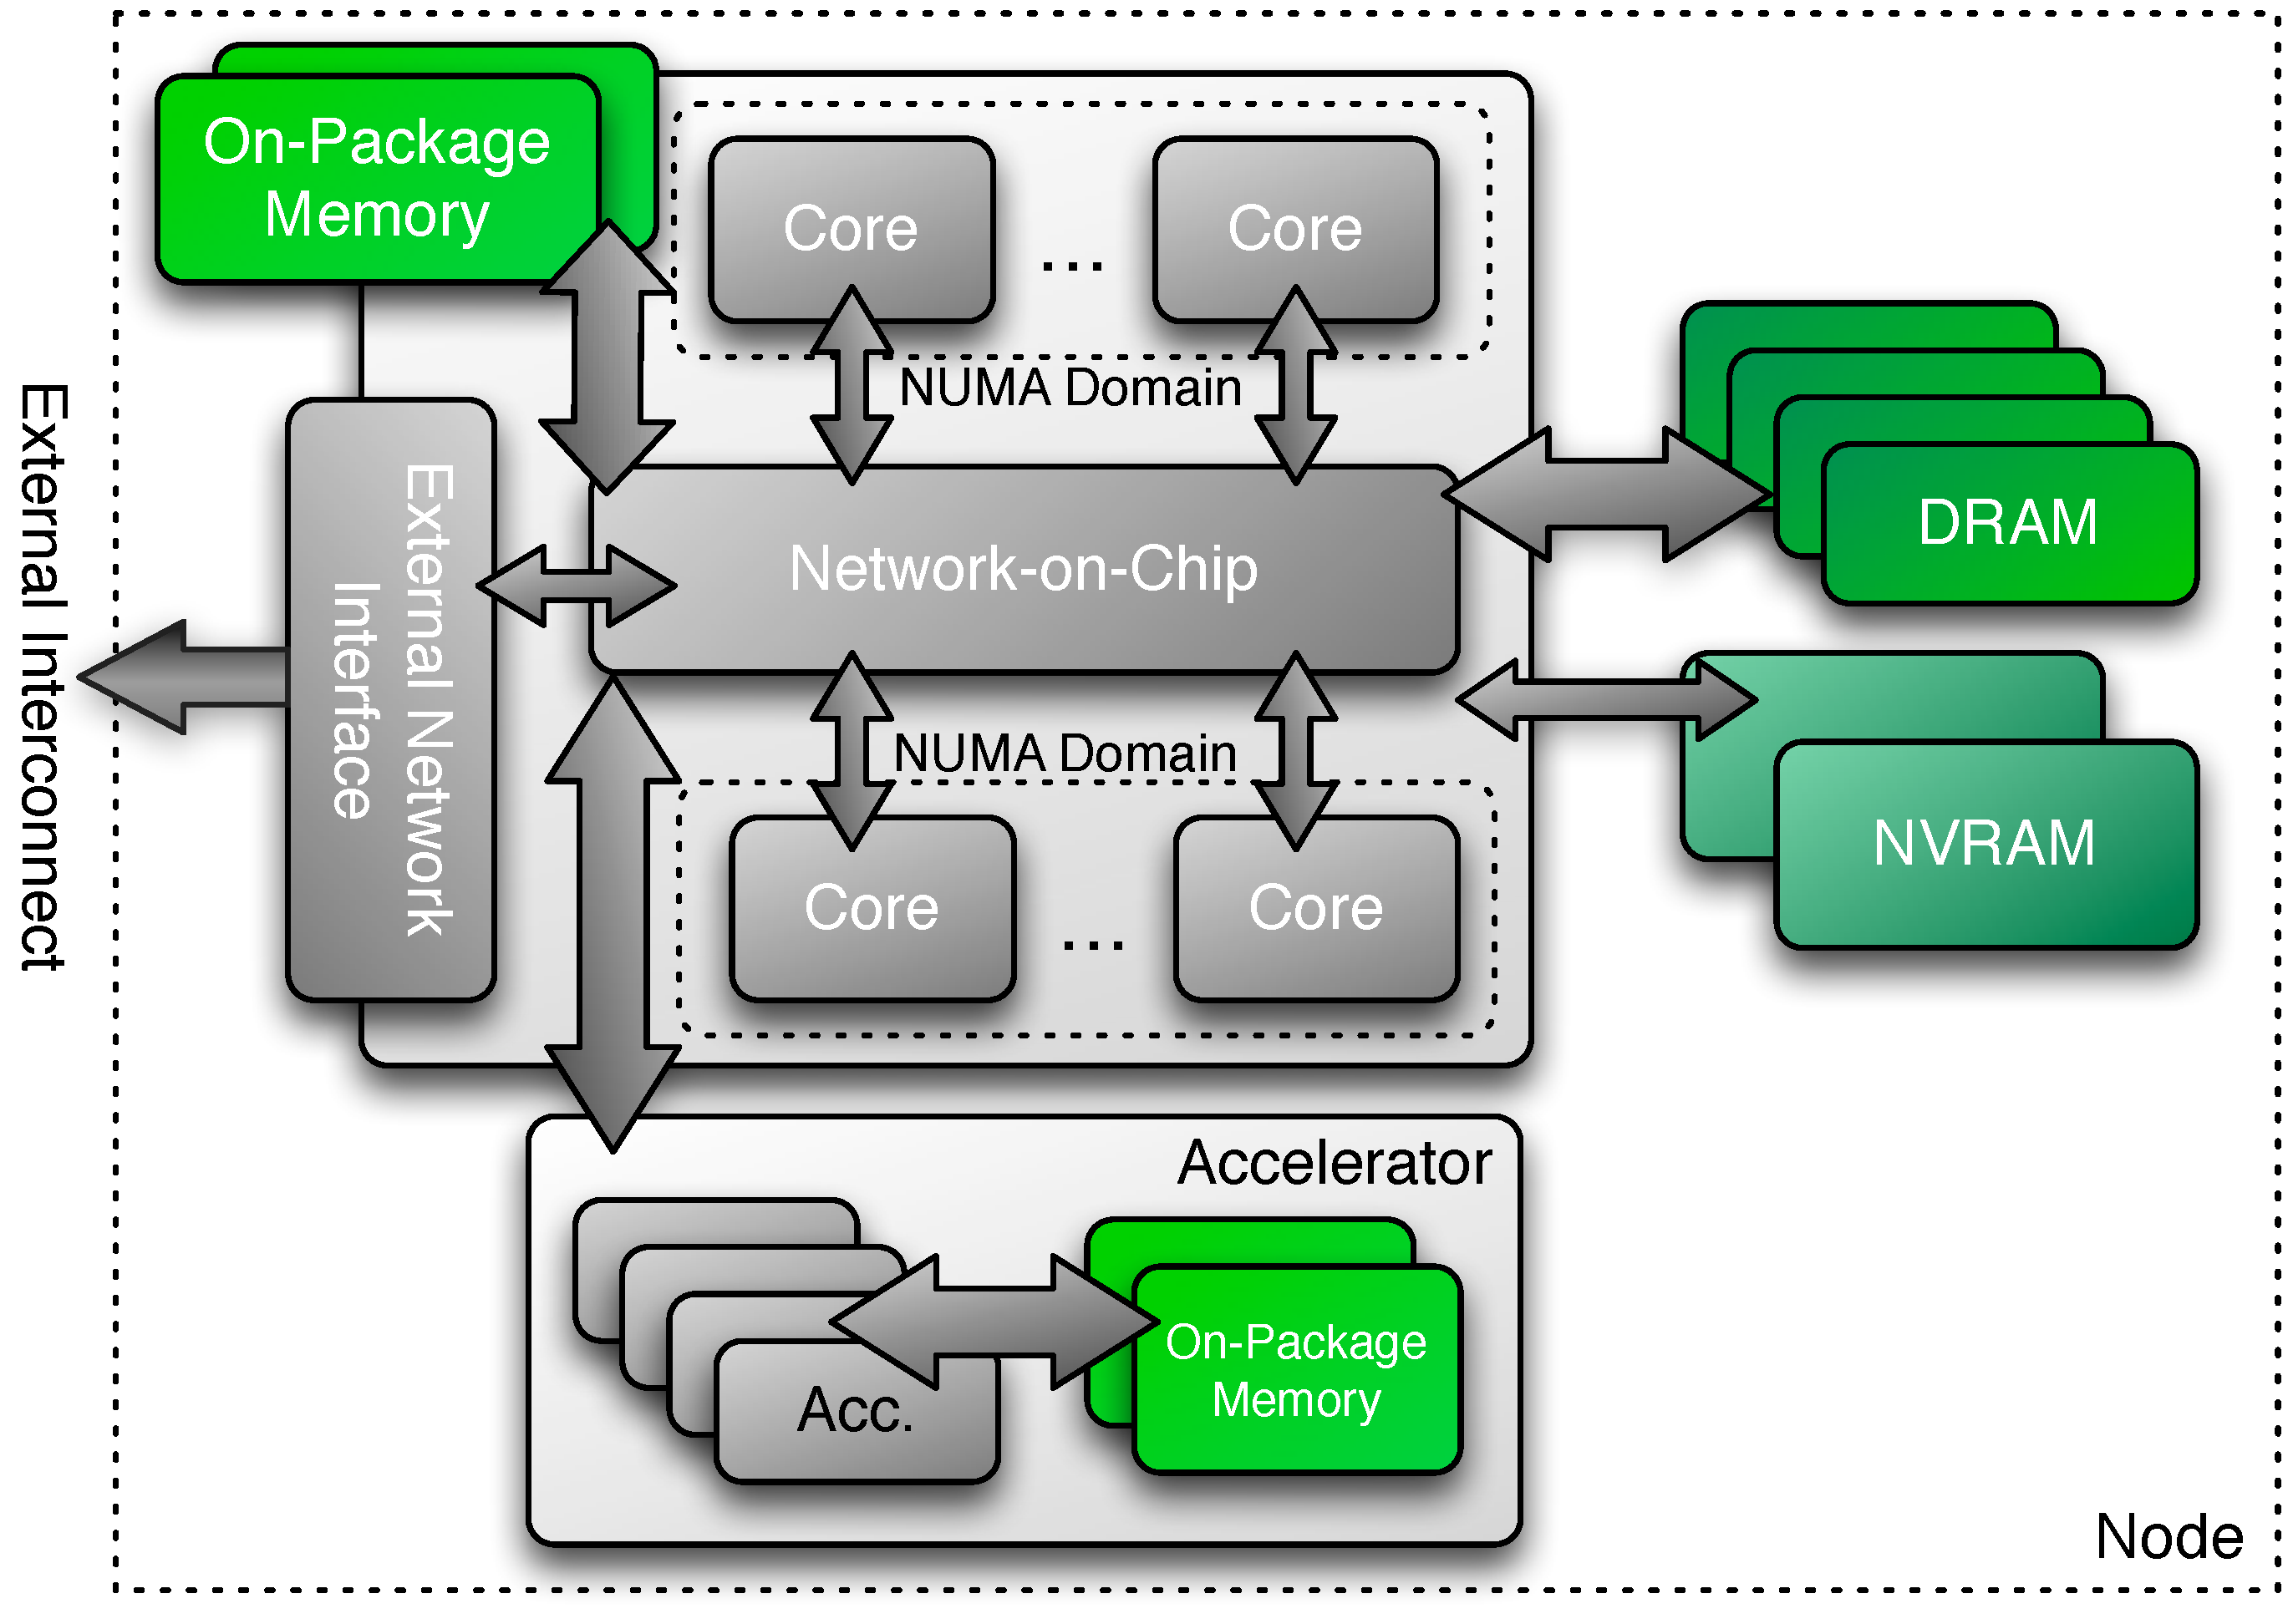
\includegraphics[width=0.75\textwidth]{figures/kokkos-memory-space}
  \end{center}

\end{frame}

%==========================================================================

\begin{frame}[fragile]{Memory spaces (1)}

  \begin{block}{Important concept: Memory spaces}
    Every view stores its data in a \textbf{memory space} set at compile time.
  \end{block}

  \vspace{10pt}

  \begin{itemize}
  \item<2->{\texttt{View<double***,}{\textit{Memory}\textbf{Space}}\texttt{> data(...);}}
  \item<3->{Available \textbf{memory spaces}: \\
            \hspace{20pt}\texttt{HostSpace, CudaSpace, CudaUVMSpace, ...} more} \\
            \hspace{20pt}Portable: \texttt{SharedSpace, SharedHostPinnedSpace}
  \item<4->{Each \textbf{execution space} has a default memory space, which is used if \textbf{Space} provided is actually an execution space}
  \item<5->{If no \texttt{Space} is provided, the view's data resides in the \textbf{default memory space} of the \textbf{default execution space}.}
  \end{itemize}

  \begin{uncoverenv}<6->
  \begin{code}[keywords={View,DefaultExecutionSpace,memory_space}]
  // Equivalent:
  View<double*> a("A",N);
  View<double*,DefaultExecutionSpace::memory_space> b("B",N);
  \end{code}
  \end{uncoverenv}
\end{frame}

%==========================================================================

\begin{frame}[fragile]{Memory spaces (2)}

  \ul{\textbf{Example: HostSpace}}

  \vspace{-3pt}

  \begin{code}[keywords={}]
View<double**, @boldHostSpace@bold> hostView(...constructor arguments...);
  \end{code}

  \vspace{-18pt}

  \begin{center}
    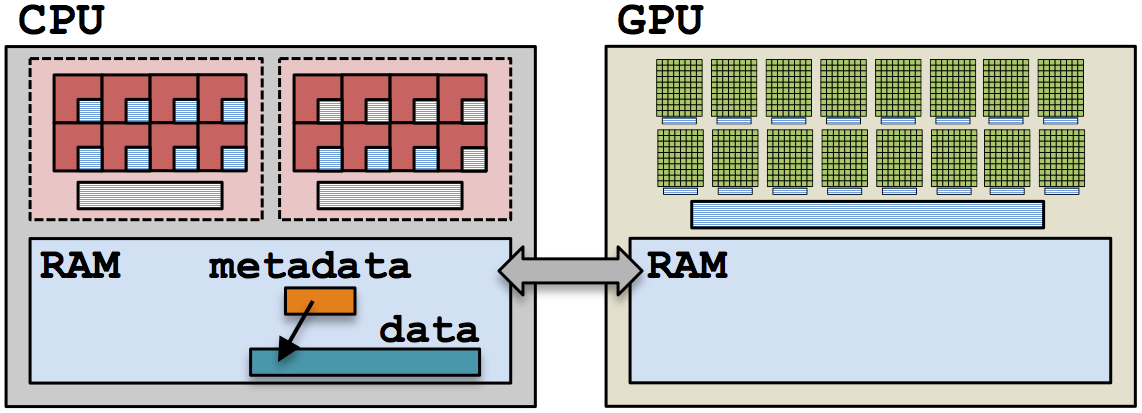
\includegraphics[width=0.70\textwidth]{figures/MemorySpaceExamples_hostSpace}
  \end{center}

  \vspace{-10pt}
  \pause

  \ul{\textbf{Example: CudaSpace}}

  \vspace{-3pt}

  \begin{code}[keywords={}]
View<double**, @boldCudaSpace@bold> view(...constructor arguments...);
  \end{code}

  \vspace{-18pt}

  \begin{center}
    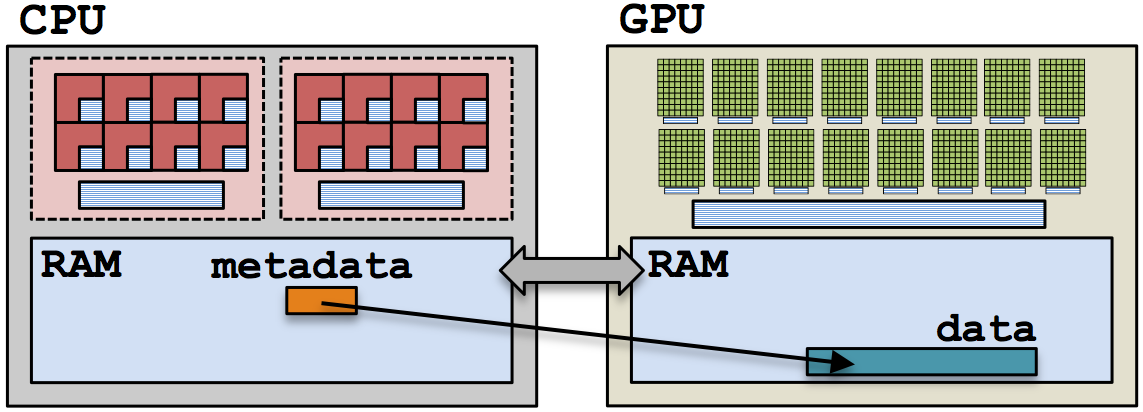
\includegraphics[width=0.70\textwidth]{figures/MemorySpaceExamples_cudaSpace}
  \end{center}

  \vspace{-10pt}

\end{frame}

%==========================================================================

\ifmedium
\begin{frame}[fragile]{Execution and Memory spaces (0)}

  \ul{\textbf{Anatomy of a kernel launch:}}

  \vspace{-10pt}

  \begin{columns}[t,onlytextwidth]

    \column{.6\textwidth}

      \begin{enumerate}
        \item{User declares views, allocating.}
        \item{User instantiates a functor with views.}
        \item{User launches \texttt{parallel\_something}:}
        \begin{itemize}
          \item{Functor is copied to the device.}
          \item{Kernel is run.}
          \item{Copy of functor on the device is released.}
        \end{itemize}
      \end{enumerate}

    \column{.40\textwidth}

      \vspace{10pt}

      \begin{code}[keywords={}]
#define KL KOKKOS_LAMBDA
View<int*, Cuda> @darkgreendev@darkgreen(...);
parallel_for("Label",N,
  KL (int i) {
    @darkgreendev@darkgreen(i) = ...;
  });
      \end{code}

      \vspace{20pt}

  \end{columns}

  \vspace{20pt}

  Note: \textbf{no deep copies} of array data are performed; \\
    \hspace{30pt}\emph{views are like pointers}.

\end{frame}
\fi

%==========================================================================

\ifmedium
\begin{frame}[fragile]{Execution and Memory spaces (1)}

  \begin{columns}[t,onlytextwidth]
    \column{.40\textwidth}

    \vspace{15pt}

    \ul{\textbf{Example: one view}}

    \vspace{5pt}

    \begin{code}[keywords={}]
#define KL KOKKOS_LAMBDA
View<int*, Cuda> @darkgreendev@darkgreen;
parallel_for("Label",N,
  KL (int i) {
    @darkgreendev@darkgreen(i) = ...;
  });
    \end{code}

    \column{.60\textwidth}

      \begin{center}
        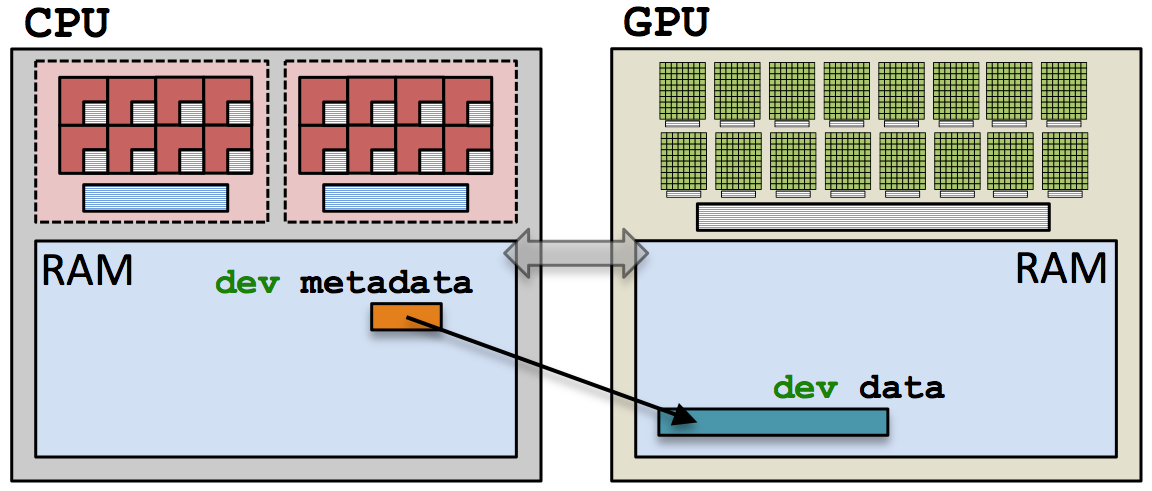
\includegraphics[width=1.00\textwidth]{figures/MemorySpaceExamples_cuda_0}
      \end{center}
      \begin{center}
        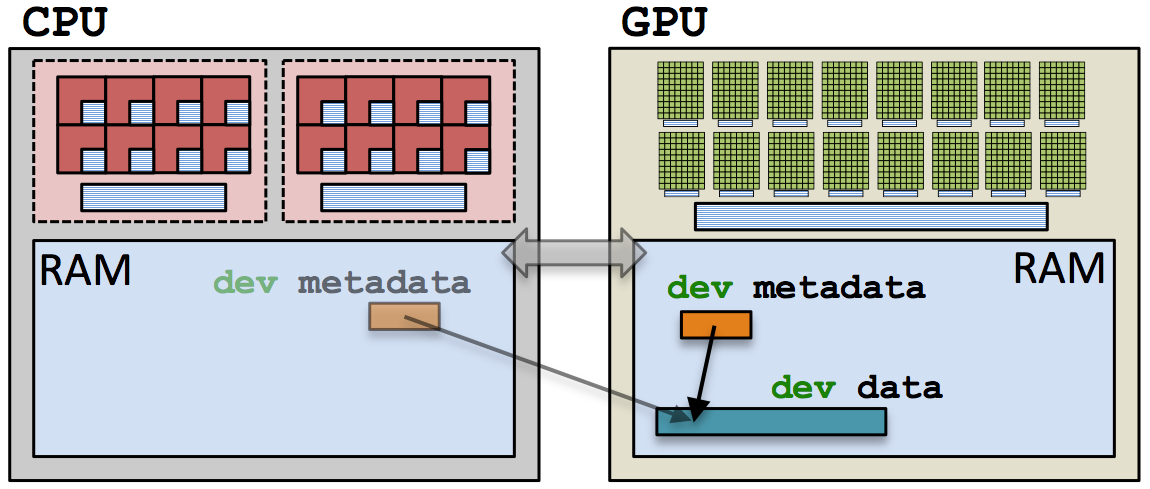
\includegraphics[width=1.00\textwidth]{figures/MemorySpaceExamples_cuda_1}
      \end{center}

  \end{columns}

\end{frame}
\fi

%==========================================================================

\ifmedium
\begin{frame}[fragile]{Execution and Memory spaces (2)}

  \begin{columns}[t,onlytextwidth]
    \column{.40\textwidth}

    \vspace{15pt}

    \ul{\textbf{Example: two views}}

    \vspace{5pt}

    \begin{code}[linebackgroundcolor={
          \btLstHL<2>{7}{red!20}
        },
        keywords={}]
#define KL KOKKOS_LAMBDA
View<int*, Cuda> @darkgreendev@darkgreen;
View<int*, Host> @bluehost@blue;
parallel_for("Label",N,
  KL (int i) {
    @darkgreendev@darkgreen(i)  = ...;
    @bluehost@blue(i) = ...;
  });
    \end{code}

    \column{.60\textwidth}

      \begin{center}
        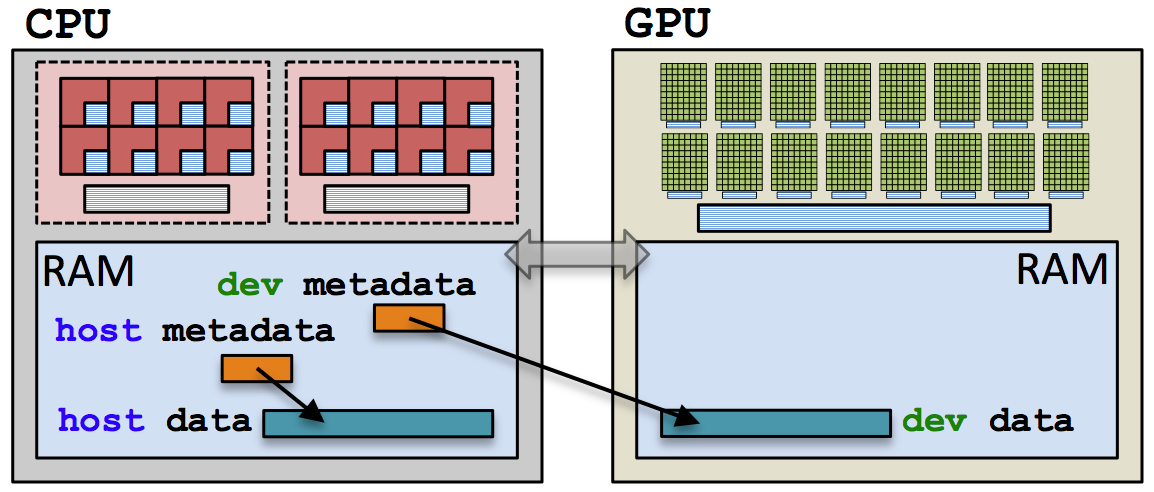
\includegraphics[width=1.00\textwidth]{figures/MemorySpaceExamples_hostCuda_0}
      \end{center}
      \begin{center}
        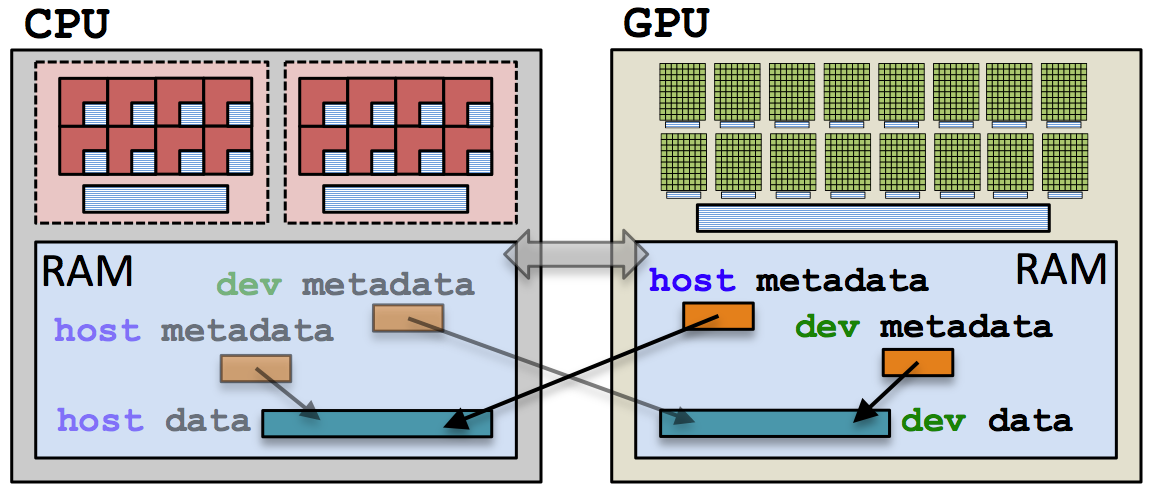
\includegraphics[width=1.00\textwidth]{figures/MemorySpaceExamples_hostCuda_1}
      \end{center}

  \end{columns}

\end{frame}
\fi

%==========================================================================

\begin{frame}[fragile]{Execution and Memory spaces (3)}

  \ul{\textbf{Example (redux): summing an array with the GPU}}

  \vspace{7pt}

  \hspace{10pt}(failed) Attempt 1: \texttt{View} lives in \texttt{CudaSpace}

  \vspace{3pt}

  \begin{code}[linebackgroundcolor={
        \btLstHL<2->{3}{red!20}
      },
      keywords={}]
View<double*, @boldCudaSpace@bold> array("array", size);
@grayfor (int64_t i = 0; i < size; ++i) {@gray
  array(i) = ...read from file...
@gray}@gray

@graydouble sum = 0;@gray
@grayKokkos::parallel_reduce("Label",@gray
  RangePolicy< @boldCuda@bold>(0, size),
  @grayKOKKOS_LAMBDA (const int64_t index, double & valueToUpdate) {@gray
    valueToUpdate += array(index);
  @gray},@gray
  @graysum);@gray
  \end{code}

  \vspace{11pt}

  \begin{textblock*}{0.5\textwidth}(0.94\textwidth,0.382\textheight)
    \only<2->{\texttt{fault}}
  \end{textblock*}

  \vspace{26pt}

\end{frame}

%==========================================================================

\begin{frame}[fragile]{Execution and Memory spaces (4)}

  \ul{\textbf{Example (redux): summing an array with the GPU}}

  \vspace{7pt}

  \hspace{10pt}(failed) Attempt 2: \texttt{View} lives in \texttt{HostSpace}

  \vspace{3pt}

  \begin{code}[linebackgroundcolor={
        \btLstHL<2-3>{10}{red!20}
      },
      keywords={}]
View<double*, @boldHostSpace@bold> array("array", size);
@grayfor (int64_t i = 0; i < size; ++i) {@gray
  array(i) = ...read from file...
@gray}@gray

@graydouble sum = 0;@gray
@grayKokkos::parallel_reduce("Label",@gray
  RangePolicy< @boldCuda@bold>(0, size),
  @grayKOKKOS_LAMBDA (const int64_t index, double & valueToUpdate) {@gray
    valueToUpdate += array(index);
  @gray},@gray
  @graysum);@gray
  \end{code}

  \vspace{3pt}

  \begin{textblock*}{0.5\textwidth}(0.82\textwidth,0.630\textheight)
    \only<2->{\texttt{illegal access}}
  \end{textblock*}

  \pause
  \pause
  \begin{columns}[t,onlytextwidth]
    \column{.35\textwidth}
      What's the solution?
    \column{.65\textwidth}
      \vspace{-25pt}
      \begin{itemize}
        \item{\texttt{SharedSpace}}
        \item{\texttt{SharedHostPinnedSpace} (skipping)}
        \item{Mirroring}
      \end{itemize}
  \end{columns}

\end{frame}

%==========================================================================

\ifmedium
\begin{frame}[fragile]{Execution and Memory spaces (5)}

  \vspace{-30pt}

  \begin{columns}[t,onlytextwidth]
    \column{.40\textwidth}

    \vspace{15pt}

    \ul{\texttt{SharedSpace}}

    \vspace{5pt}

    \begin{code}[keywords={}]
#define KL KOKKOS_LAMBDA
View<double*,
     @boldSharedSpace@bold> @darkgreenarray@darkgreen;
@darkgreenarray@darkgreen = ...from file...
double sum = 0;
parallel_reduce("Label", N,
  KL (int i, double & d) {
    d += @darkgreenarray@darkgreen(i);
  },
  sum);
    \end{code}

    \vspace{5pt}

    %{\color{red}Warning:} \\ \hspace{10pt}Performance penalty

    \column{.55\textwidth}

      \begin{center}
        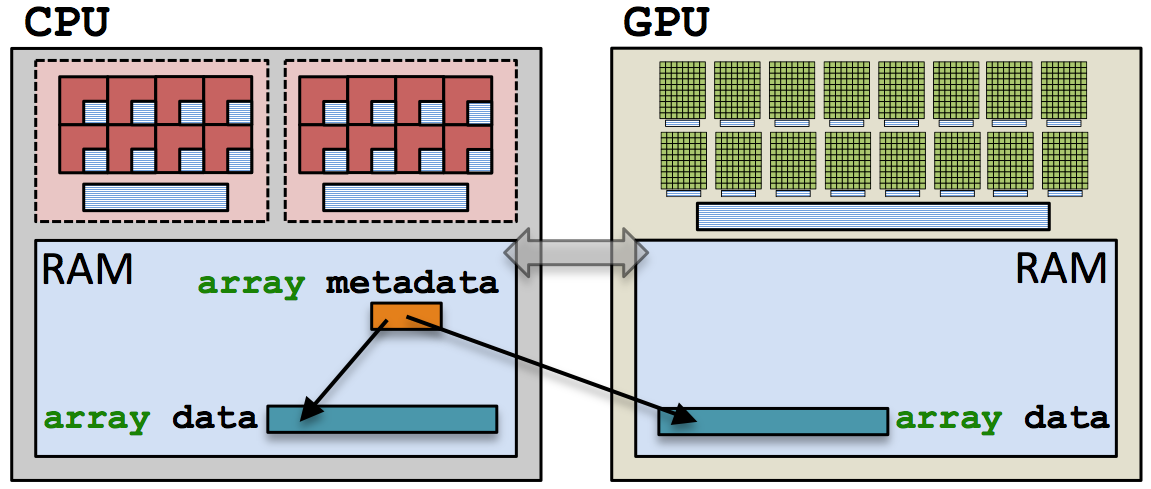
\includegraphics[width=0.95\textwidth]{figures/MemorySpaceExamples_uvm_0}
      \end{center}
      \begin{center}
        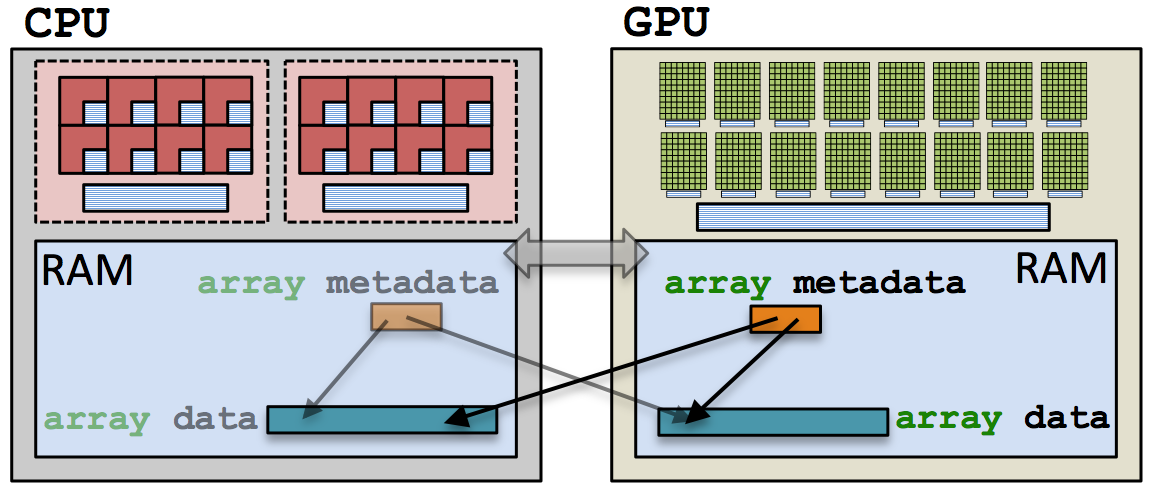
\includegraphics[width=0.95\textwidth]{figures/MemorySpaceExamples_uvm_1}
      \end{center}

  \end{columns}

  \vspace{10pt}

  Cuda runtime automatically handles data movement,
  \\ at a \textbf{performance hit}.

\end{frame}
\fi

\begin{comment}
\begin{frame}[fragile]{Exercise: CG-Solve}

  \textbf{Exercise}: Find $x$ in $b = A * x$

  Getting set up in your home directory:
  \begin{code}
    mkdir Kokkos
    cd Kokkos
    git clone https://github.com/kokkos/kokkos
    git clone https://github.com/kokkos/kokkos-tutorials
  \end{code}

  \vspace{5pt}
  Find the exercise in the kokkos-turoials/Exercises/cg-solve folder.


  \vspace{5pt}
  The Begin subdirectory contains the code. Only cg\_solve.cpp needs modifications.

  \vspace{5pt}
  Look for EXERCISE comments to find places to modify.

\end{frame}

%==========================================================================

\begin{frame}[fragile]{Exercise \#1: include, initialize, finalize Kokkos}

  The \textbf{first step} in using Kokkos is to include, initialize, and finalize:

  \begin{code}
#include <Kokkos_Core.hpp>
int main(int argc, char* argv[]) {
  /* ... do any necessary setup (e.g., initialize MPI) ... */
  Kokkos::initialize(argc, argv);
  {
  /* ... do computations ... */
  }
  Kokkos::finalize();
  return 0;
}
  \end{code}

  \vspace{7pt}

  (Optional) Command-line arguments or environment variables:

  \vspace{3pt}

	\begin{tabular}{| p{0.5\textwidth} | p{0.5\textwidth} |}
    \hline
	  \texttt{--kokkos-threads=INT} or \texttt{KOKKOS\_NUM\_THREADS} & total number of threads \\
    \hline
	  \texttt{--kokkos-device-id=INT} or \texttt{KOKKOS\_DEVICE\_ID} & device (GPU) ID to use \\
    \hline
  \end{tabular}

\end{frame}

%==========================================================================



\begin{frame}[fragile]{Exercise: Compiling}

\ul{\textbf{Compiling for CPU}}

\vspace{-3pt}
  \begin{small}
  \begin{code}
    cmake -B build_openmp -D Kokkos_ENABLE_OPENMP=ON
    cmake --build build_openmp -j
  \end{code}
  Optional: configure with \texttt{Kokkos\_ARCH\_NATIVE=ON} or specify explicitly the target architecture
  \end{small}

%  \hspace{10pt} {\tiny \url{https://github.com/kokkos/kokkos/wiki/Compiling#table-43-architecture-variables}}

\ul{\textbf{Running on CPU} with OpenMP back-end}

\vspace{-3pt}
  \begin{small}
  \begin{code}
  # Set OpenMP affinity
  export OMP_NUM_THREADS=8
  export OMP_PROC_BIND=spread OMP_PLACES=threads
  # Print example command line options:
  ./cg\_solve.exe -h
  # Run with defaults on CPU
  ./cg\_solve.exe
  # Run larger problem
  ./cg\_solve.exe 200 200
  \end{code}
  \end{small}

\ul{\textbf{Things to try:}}
  \begin{small}
  \begin{itemize}
  \itemsep0em
  \item Vary number of threads
  \item Vary problem size
  \item Compare Serial backend performance to unmodified code
  \end{itemize}
  \end{small}
\end{frame}

\begin{frame}[fragile]{Exercise: Compiling}

\ul{\textbf{Compiling for GPU}}

\vspace{-3pt}
  \begin{small}
  \begin{code}
    cmake -B build_openmp -D Kokkos_ENABLE_OPENMP=ON
    cmake --build build_openmp -j
  \end{code}
  Optional: configure with \texttt{Kokkos\_ARCH\_NATIVE=ON} or specify explicitly the target architecture
  \end{small}

%  \hspace{10pt} {\tiny \url{https://github.com/kokkos/kokkos/wiki/Compiling#table-43-architecture-variables}}

\ul{\textbf{Things to try:}}
  \begin{small}
  \begin{itemize}
  \itemsep0em
  \item Vary number of iterations
  \item Vary problem size
  \item Compare performance to CPU runs? What is the ratio compared to expected bandwidth ratio?
  \end{itemize}
  \end{small}
\end{frame}
\end{comment}

%==========================================================================
%==========================================================================

\begin{frame}[fragile]{Views, Spaces, and Mirrors}

  \begin{block}{Important concept: Mirrors}
    Mirrors are views of equivalent arrays residing in possibly different memory spaces.
  \end{block}

  \vspace{3pt}
  \pause

  \ul{\textbf{Mirroring schematic}}

  \vspace{-3pt}

  \begin{code}[keywords={view_type}]
Kokkos::View<double**, @boldSpace@bold> @darkgreenview@darkgreen(...);
auto @darkredhostView@darkred = @boldKokkos::create_mirror_view@bold(@darkgreenview@darkgreen);
  \end{code}

  \vspace{-8pt}

  \begin{center}
    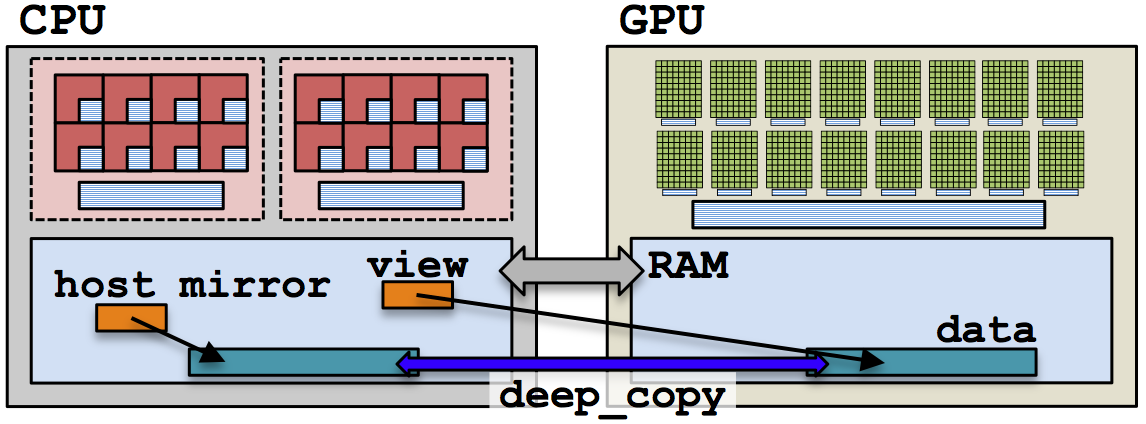
\includegraphics[width=0.70\textwidth]{figures/MemorySpaceExamples_mirrors}
  \end{center}

  \vspace{-10pt}

\end{frame}

%==========================================================================

\begin{frame}[fragile]{Mirroring pattern}

  \begin{enumerate}
    \item<+->{\textbf{Create} a {\color{darkgreen}\texttt{view}}'s array in some memory space. \\

      \vspace{-5pt}
      \begin{code}[keywords={view_type}]
  Kokkos::View<double*, @boldSpace@bold> @darkgreenview@darkgreen(...);
      \end{code}
      \vspace{-4pt}

  }
    \item<+->{\textbf{Create} {\color{darkred}\texttt{hostView}}, a \textit{mirror} of the {\color{darkgreen}\texttt{view}}'s array residing in the host memory space. \\

      \vspace{-5pt}
      \begin{code}[keywords={view_type}]
  auto @darkredhostView@darkred = @boldKokkos::create_mirror_view@bold(@darkgreenview@darkgreen);
      \end{code}
      \vspace{-4pt}

  }
    \item<+->{\textbf{Populate} {\color{darkred}\texttt{hostView}} on the host (from file, etc.).}
    \item<+->{\textbf{Deep copy} {\color{darkred}\texttt{hostView}}'s array to {\color{darkgreen}\texttt{view}}'s array. \\

      \vspace{-5pt}
      \begin{code}[keywords={}]
  Kokkos::@bolddeep_copy@bold(@darkgreenview@darkgreen, @darkredhostView@darkred);
      \end{code}
      \vspace{-4pt}

  }
    \item<+->{\textbf{Launch} a kernel processing the {\color{darkgreen}\texttt{view}}'s array. \\

      \vspace{-5pt}
      \begin{code}[keywords={}]
  Kokkos::parallel_for("Label",
    RangePolicy< @boldSpace@bold>(0, size),
    KOKKOS_LAMBDA (...) { use and change @darkgreenview@darkgreen });
      \end{code}
      \vspace{-4pt}

  }
    \item<+->{If needed, \textbf{deep copy} the {\color{darkgreen}\texttt{view}}'s updated array back to the {\color{darkred}\texttt{hostView}}'s array to write file, etc. \\

      \vspace{-5pt}
      \begin{code}[keywords={}]
  Kokkos::@bolddeep_copy@bold(@darkredhostView@darkred, @darkgreenview@darkgreen);
      \end{code}
      \vspace{-4pt}

  }
  \end{enumerate}

\end{frame}

%==========================================================================

\begin{frame}[fragile]{Mirrors of \texttt{View}s in \texttt{HostSpace}}

  What if the \texttt{View} is in \texttt{HostSpace} too?  Does it make a copy?

  \begin{code}[keywords={}]
Kokkos::View<double*, @boldSpace@bold> @darkgreenview@darkgreen("test", 10);
auto @darkredhostView@darkred = @boldKokkos::create_mirror_view@bold(@darkgreenview@darkgreen);
  \end{code}

  \begin{itemize}
    \item{\texttt{create\_mirror\_view} allocates data only if the host process cannot access {\color{darkgreen}view}'s data, otherwise {\color{darkred}hostView} references the same data.}
    \item{\texttt{create\_mirror} \textbf{always} allocates data.}
    \item{\texttt{create\_mirror\_view\_and\_copy} allocates data if necessary and also \textbf{copies} data.}
  \end{itemize}

  Reminder: Kokkos \emph{never} performs a \textbf{hidden deep copy}.

  \vspace{-5pt}

\end{frame}

%==========================================================================

\begin{frame}[fragile]{Exercise \#3: Flat Parallelism on the GPU, Views and Host Mirrors}

  \textbf{Details}:
  \begin{scriptsize}
  \begin{itemize}
\item Location: \ExerciseDirectory{03/Begin}
\item Add HostMirror Views and deep copy
\item Make sure you use the correct view in initialization and Kernel
\end{itemize}
  \end{scriptsize}

\begin{code}
  # Compile for CPU
  cmake -B build_openmp -DKokkos_ENABLE_OPENMP=ON
  cmake --build build_openmp
  # Run on CPU
  ./build_openmp/03_Exercise -S 26
  # Note the warnings, set appropriate environment variables
  # Compile for GPU
  cmake -B build_cuda -DKokkos_ENABLE_CUDA=ON
  cmake --build build_cuda
  # Run on GPU
  ./build_cuda/03_Exercise -S 26
\end{code}

  \ul{\textbf{Things to try:}}
  \begin{scriptsize}
  \begin{itemize}
  \item Vary problem size and number of rows (-S ...; -N ...)
  \item Change number of repeats (-nrepeat ...)
  \item Compare behavior of CPU vs GPU
  \end{itemize}
  \end{scriptsize}



\end{frame}

%==========================================================================

\begin{frame}[fragile]{View and Spaces Section Summary}

  \begin{itemize}
    \item{Data is stored in \texttt{Views} that are ``pointers'' to \textbf{multi-dimensional arrays} residing in \textbf{memory spaces}.}
    \item{\texttt{Views} \textbf{abstract away} platform-dependent allocation, (automatic) deallocation, and access.}
    \item{\textbf{Heterogeneous nodes} have one or more memory spaces.}
    \item{\textbf{Mirroring} is used for performant access to views in host and device memory.}
    \item{Heterogeneous nodes have one or more \textbf{execution spaces}.}
    \item{You \textbf{control where} parallel code is run by a template parameter on the execution policy, or by compile-time selection of the default execution space.}
  \end{itemize}

\end{frame}


\begin{frame}[fragile]

  {\huge Managing memory access patterns \\ for performance portability}

  \vspace{20pt}

  \textbf{Learning objectives:}
  \begin{itemize}
    \item{How the \texttt{View}'s \texttt{Layout} parameter controls data layout.}
    \item{How memory access patterns result from Kokkos mapping parallel work indices \textbf{and} layout of multidimensional array data}
    \item{Why memory access patterns and layouts have such a performance impact (caching and coalescing).}
    \item{See a concrete example of the performance of various memory configurations.}
  \end{itemize}

  \vspace{-20pt}

\end{frame}

%==========================================================================

\begin{frame}[fragile]{Example: inner product (0)}

  \begin{code}[keywords={}]
Kokkos::parallel_reduce("Label", 
  RangePolicy<ExecutionSpace>(0, N),
  KOKKOS_LAMBDA (const size_t row, double & valueToUpdate) {
    double thisRowsSum = 0;
    for (size_t entry = 0; entry < M; ++entry) {
      thisRowsSum += @blueA@blue(row, entry) * @darkgreenx@darkgreen(entry);
    }
    valueToUpdate += @darkredy@darkred(row) * thisRowsSum;
  }, @orangeresult@orange);
  \end{code}

  \vspace{-20pt}

  \begin{center}
    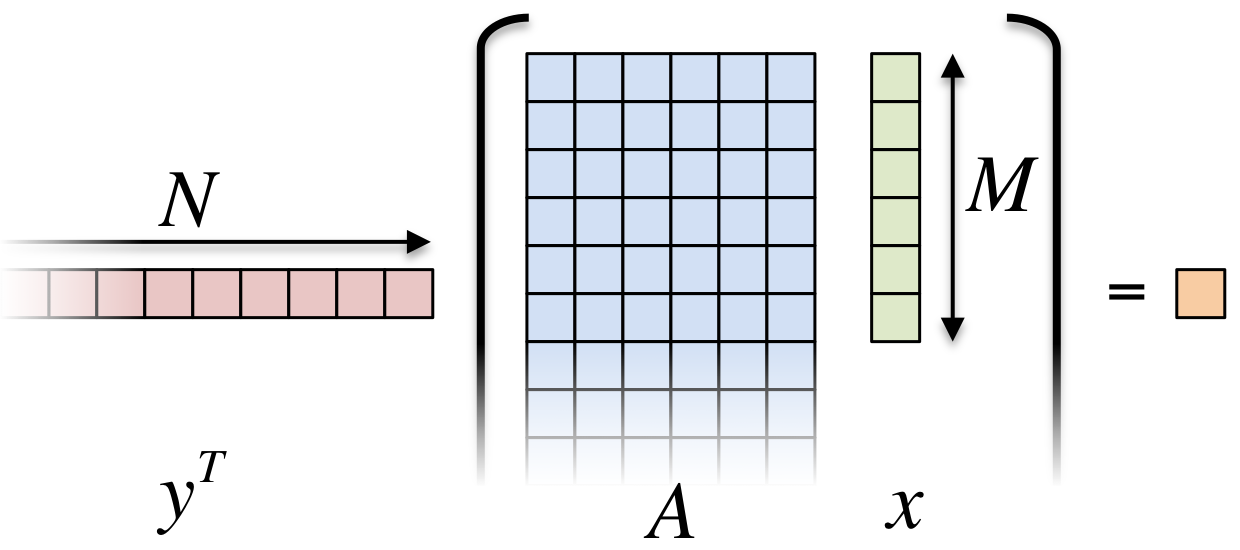
\includegraphics[width=0.8\textwidth]{figures/InnerProductExample_LayoutIntro}
  \end{center}

  \pause
  \vspace{-8pt}

 \textbf{Driving question:} How should {\color{blue}\texttt{A}} be laid out in memory?

  \vspace{8pt}

\end{frame}

%==========================================================================

\begin{frame}[fragile]{Example: inner product (1)}

  Layout is the mapping of multi-index to memory:

  \vspace{-10pt}

  \begin{columns}[t,onlytextwidth]
    \column{.40\textwidth}

      \vspace{20pt}

      \ul{\textbf{LayoutLeft}} \\
      \vspace{3pt}
      \hspace{10pt} in 2D, ``column-major''

      \vspace{50pt}

      \ul{\textbf{LayoutRight}} \\
      \vspace{3pt}
      \hspace{10pt} in 2D, ``row-major''
    \column{.60\textwidth}
      \begin{center}
        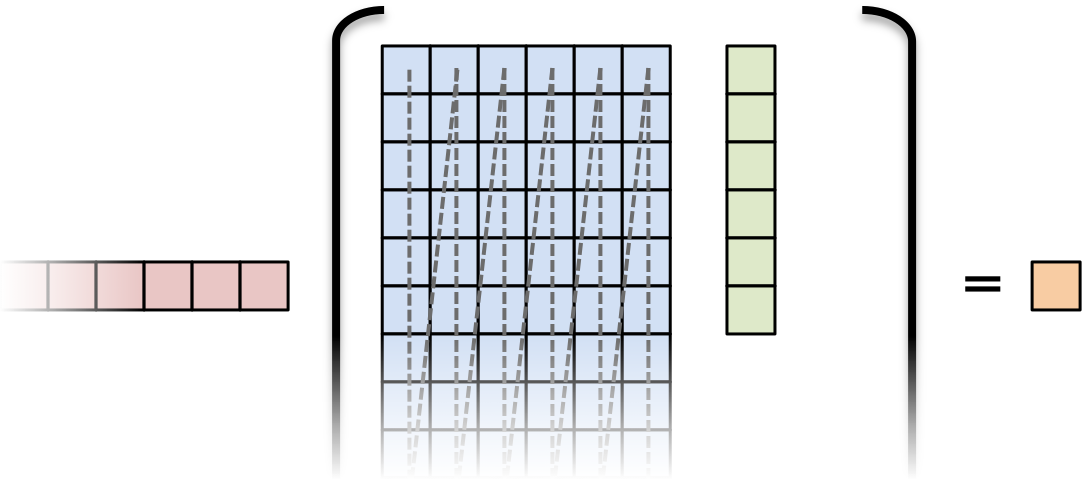
\includegraphics[width=1.00\textwidth]{figures/InnerProductExample_LayoutLeft}
        \\
        \vspace{10pt}
        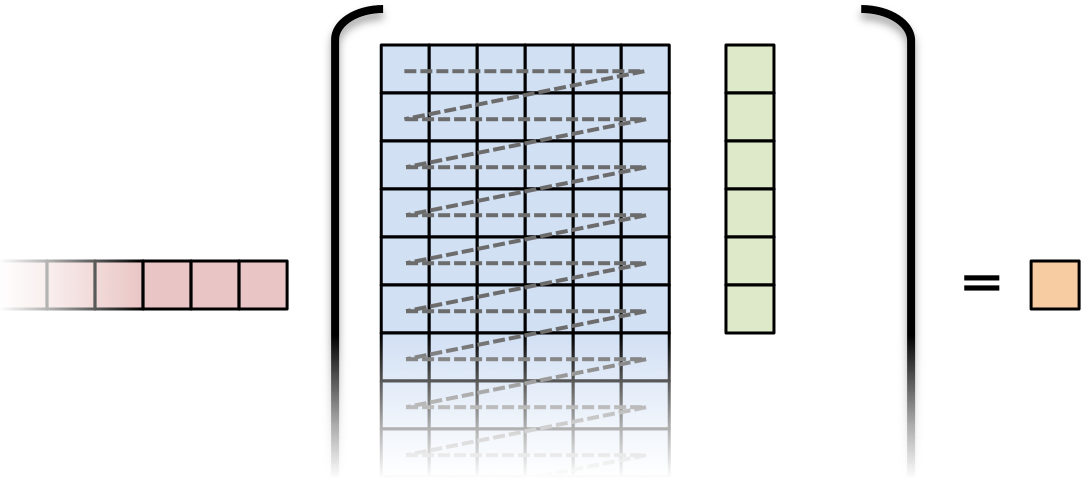
\includegraphics[width=1.00\textwidth]{figures/InnerProductExample_LayoutRight}
      \end{center}
  \end{columns}

\end{frame}

%==========================================================================

\begin{frame}[fragile]{Layout}

  \begin{block}{Important concept: Layout}
    Every \texttt{View} has a multidimensional array \texttt{Layout} set at compile-time.
  \end{block}

  \vspace{5pt}

  \begin{code}[frame=single, keywords={}]
View<double***, @boldLayout@bold, Space> name(...);
  \end{code}

  \pause
  \vspace{-5pt}

  \begin{itemize}
    \item{Most-common layouts are \texttt{LayoutLeft} and \texttt{LayoutRight}. \\
      \hspace{10pt} \texttt{LayoutLeft}: left-most index is stride 1.\\
      \hspace{10pt} \texttt{LayoutRight}: right-most index is stride 1.}
    \item{If no layout specified, default for that memory space is used. \\
      \hspace{10pt} \texttt{LayoutLeft} for \texttt{CudaSpace}, \texttt{LayoutRight} for \texttt{HostSpace}.}
    \item{Layouts are extensible: $\approx$ 50 lines}
    \item{Advanced layouts: \texttt{LayoutStride}, \texttt{LayoutTiled}, ...}
  \end{itemize}

  \vspace{-15pt}

\end{frame}

%==========================================================================

\begin{frame}[fragile]{Exercise \#4: Inner Product, Flat Parallelism}

  \textbf{Details}:
  \begin{small}
  \begin{itemize}
\item Location: \ExerciseDirectory{04/Begin}
\item Replace \texttt{``N''} in parallel dispatch with \texttt{RangePolicy<ExecSpace>}
\item Add \texttt{MemSpace} to all \texttt{Views} and \texttt{Layout} to \texttt{A}
\item Experiment with the combinations of \texttt{ExecSpace}, \texttt{Layout} to view performance
\end{itemize}
  \end{small}


\ul{\textbf{Things to try:}}
  \begin{small}
  \begin{itemize}
  \item Vary problem size and number of rows (-S ...; -N ...)
  \item Change number of repeats (-nrepeat ...)
  \item Compare behavior of CPU vs GPU
  \item On GPUs, compare using \texttt{SharedSpace} vs using the default memory space, i.e, not providing an explicit memory space.
  \item Check what happens if \texttt{MemSpace} and \texttt{ExecSpace} do not match.
  \end{itemize}
  \end{small}
\end{frame}

%==========================================================================

\begin{frame}[fragile]{Exercise \#4: Inner Product, Flat Parallelism}


  \vspace{-10pt}

    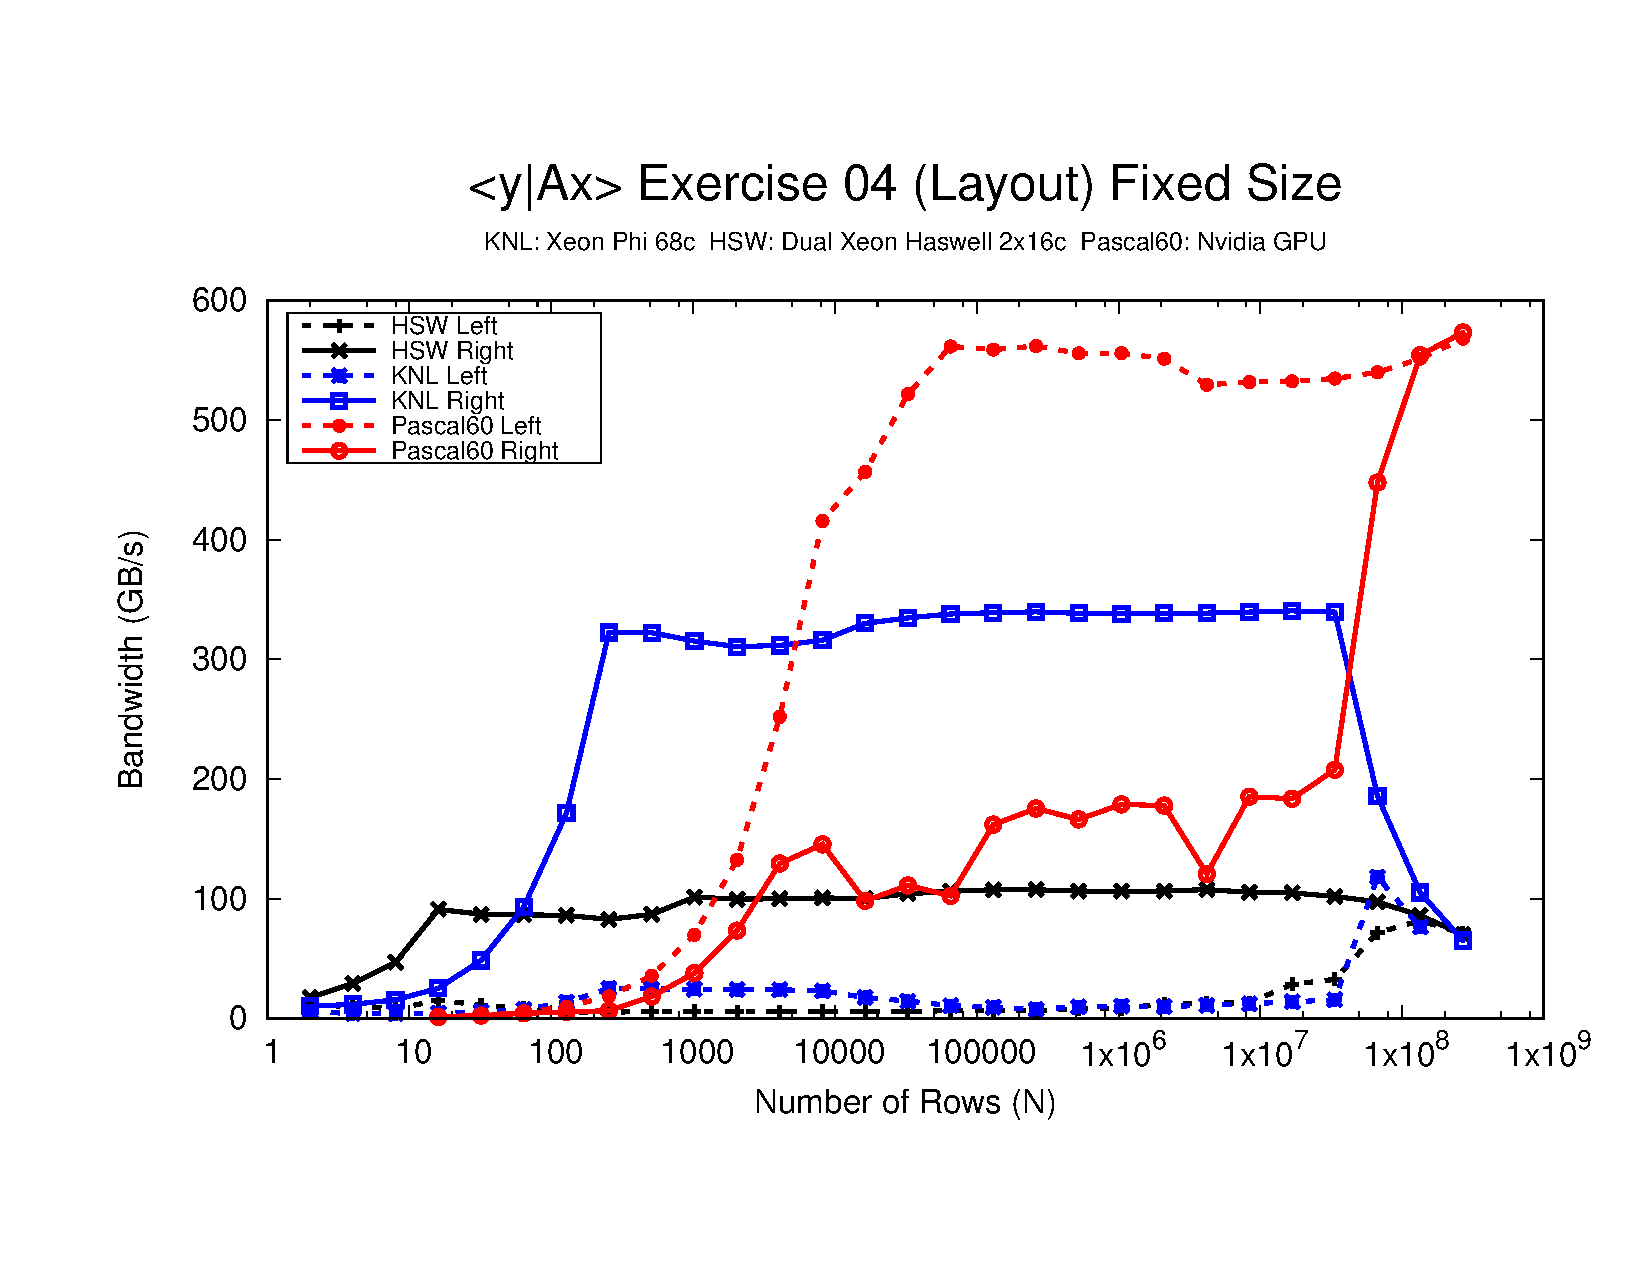
\includegraphics[viewport=1.25in 3.0in 10in 6in, width=0.95\textwidth]{figures/Exercise04-Performance.pdf}

  \vspace{-15pt}

  \begin{textblock*}{0.5\textwidth}(0.97\textwidth,0.50\textheight)
    \textbf{\LARGE Why?}
  \end{textblock*}

\end{frame}

%==========================================================================

\begin{frame}[fragile]{Caching and coalescing (0)}

  \ul{\textbf{Thread independence:}}

  \begin{code}[keywords={}]
operator()(int index, double & valueToUpdate) const {
  const double d = _data(index);
  valueToUpdate += d;
}
  \end{code}

  Question: once a thread reads \texttt{d}, does it need to wait?

  \pause

  \begin{itemize}
    \item \textbf{CPU} threads are independent.
       \begin{itemize}
	   \item i.e., threads may execute at any rate.
       \end{itemize}
  \item<3->{\textbf{GPU} threads execute synchronized. 
	  \begin{itemize}
	     \item i.e., threads in groups can/must execute instructions together.
	  \end{itemize}}
  \end{itemize}

  \pause
  \pause

	In particular, all threads in a group (\emph{warp} or \emph{wavefront}) must finished their loads before \emph{any} thread can move on.

  \vspace{5pt}

  \pause

  So, \textbf{how many cache lines} must be fetched before threads can move on?

\end{frame}

%==========================================================================

\ifmedium
\begin{frame}[fragile]{Caching and coalescing (1)}

  \ul{\textbf{CPUs}: few (independent) cores with separate caches:}

  \vspace{-10pt}

  \begin{columns}[t,onlytextwidth]
    \column{.50\textwidth}
      \begin{center}
        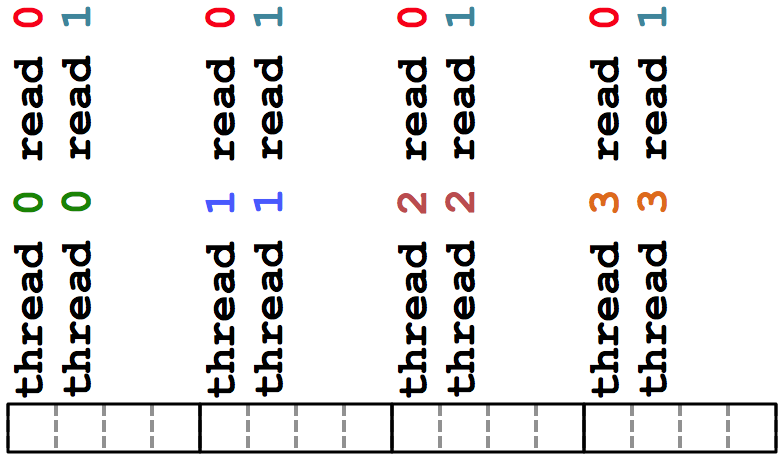
\includegraphics[width=0.80\textwidth]{figures/MemoryAccessPatterns_Caching}
      \end{center}
    \column{.50\textwidth}
      \begin{center}
        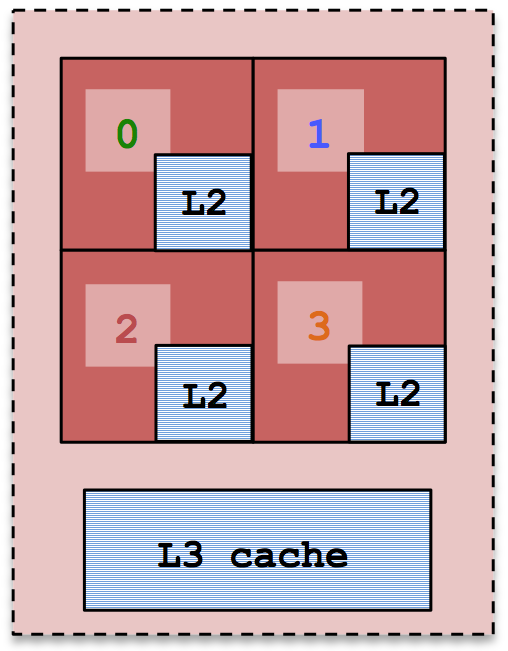
\includegraphics[width=0.38\textwidth]{figures/Schematics_CPU_withThreadIndices_justOne}
      \end{center}
  \end{columns}

  \vspace{5pt}
  \pause

  \ul{\textbf{GPUs}: many (synchronized) cores with a shared cache:}

  \vspace{-10pt}

  \begin{columns}[t,onlytextwidth]
    \column{.50\textwidth}
      \begin{center}
        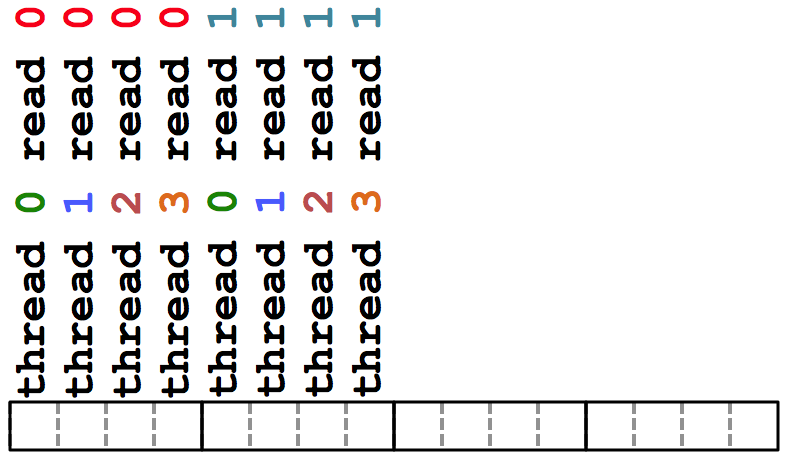
\includegraphics[width=0.80\textwidth]{figures/MemoryAccessPatterns_Coalescing}
      \end{center}
    \column{.50\textwidth}
      \begin{center}
        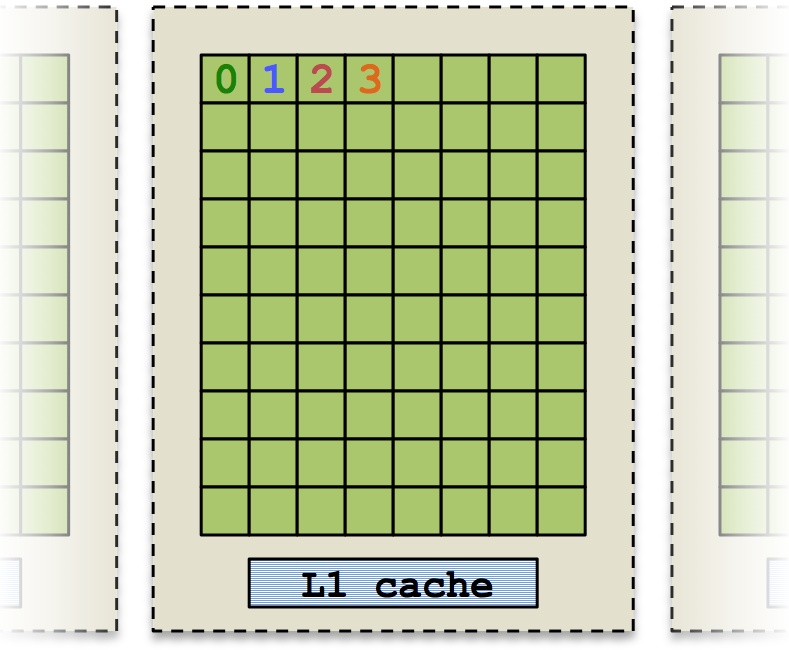
\includegraphics[width=0.60\textwidth]{figures/Schematics_GPU_withThreadIndices}
      \end{center}
  \end{columns}

\end{frame}
\fi

%==========================================================================

\begin{frame}[fragile]{Caching and coalescing (2)}

  \begin{block}{Important point}
    For performance, accesses to views in \texttt{HostSpace} must be \textbf{cached}, while access to views in \texttt{CudaSpace} must be \textbf{coalesced}.
  \end{block}

  \vspace{5pt}

  \textbf{Caching}: if thread \texttt{t}'s current access is at position \texttt{i}, \\
  \hspace{20pt} thread \texttt{t}'s next access should be at position \texttt{i+1}.

  \vspace{5pt}

  \textbf{Coalescing}: if thread \texttt{t'}s current access is at position \texttt{i}, \\
  \hspace{20pt} thread \texttt{t+1}'s current access should be at position \texttt{i+1}.

  \pause

  \begin{alertblock}{Warning}
    Uncoalesced access on GPUs and non-cached loads on CPUs \emph{greatly} reduces performance (can be 10X)
  \end{alertblock}

\end{frame}

%==========================================================================

\ifmedium
\begin{frame}[fragile]{Mapping indices to cores (0)}

  Consider the array summation example:

  \begin{code}[keywords={}]
View<double*, @boldSpace@bold> data("data", size);
...populate data...

double sum = 0;
Kokkos::parallel_reduce("Label", 
  RangePolicy< @boldSpace@bold>(0, size),
  KOKKOS_LAMBDA (const size_t index, double & valueToUpdate) {
    valueToUpdate += data(index);
  },
  sum);
  \end{code}

  \vspace{0pt}

  Question: is this cached (for \texttt{OpenMP}) and coalesced (for \texttt{Cuda})?

  \pause
  \vspace{5pt}

  Given \texttt{P} threads, \textbf{which indices} do we want thread 0 to handle?

  \vspace{-15pt}

  \begin{columns}[t,onlytextwidth]
    \column{.50\textwidth}
      \begin{center}
        Contiguous: \\
        \texttt{0, 1, 2, ..., N/P}
      \end{center}
    \column{.50\textwidth}
      \begin{center}
        Strided: \\
        \texttt{0, N/P, 2*N/P, ...}
      \end{center}
  \end{columns}

  \vspace{-10pt}
  \pause

  \begin{columns}[t,onlytextwidth]
    \column{.50\textwidth}
      \begin{center}
        \textbf{CPU}
      \end{center}
    \column{.50\textwidth}
      \begin{center}
        \textbf{GPU}
      \end{center}
  \end{columns}

  \vspace{-10pt}

  \begin{center}
    \textbf{Why?}
  \end{center}

  \vspace{-10pt}

\end{frame}
\fi

%==========================================================================

\ifmedium
\begin{frame}[fragile]{Mapping indices to cores (1)}

  \ul{\textbf{Iterating for the execution space:}}

  \begin{code}[keywords={}]
operator()(int index, double & valueToUpdate) const {
  const double d = _data(index);
  valueToUpdate += d;
}
  \end{code}

  \vspace{5pt}

  As users we don't control how indices are mapped to threads, so how do we achieve good memory access?

  \pause
  \vspace{3pt}

  \begin{block}{Important point}
    Kokkos maps indices to cores in \textbf{contiguous chunks} on CPU execution spaces, and \textbf{strided} for \texttt{Cuda}.
  \end{block}

\end{frame}
\fi

%==========================================================================

\begin{frame}[fragile]{Mapping indices to cores (2)}

  \begin{block}{Rule of Thumb}
    Kokkos index mapping and default layouts provide efficient access if \textbf{iteration indices} correspond to the \textbf{first index} of array.
  \end{block}

  \vspace{10pt}

  \textbf{Example:}

  \vspace{5pt}

  \begin{code}[keywords={}, frame=single]
  View<double***, ...> view(...);
  ...
  Kokkos::parallel_for("Label", ... ,
    KOKKOS_LAMBDA (int workIndex) {
      ...
      @darkredview(..., ... , workIndex ) = ...@darkred;
      @darkredview(... , workIndex, ... ) = ...@darkred;
      @darkgreenview(workIndex, ... , ... ) = ...@darkgreen;
    });
  ...
  \end{code}

\end{frame}

%==========================================================================

\iffull
\begin{frame}[fragile]{Example: inner product (2)}

  \begin{block}{Important point}
    Performant memory access is achieved by Kokkos mapping parallel work indices \textbf{and} multidimensional array layout \emph{appropriately for the architecture}.
  \end{block}

  \pause
  \vspace{3pt}

  \ul{\textbf{Analysis: row-major} (\texttt{LayoutRight})}

  \vspace{-10pt}

  \begin{center}
    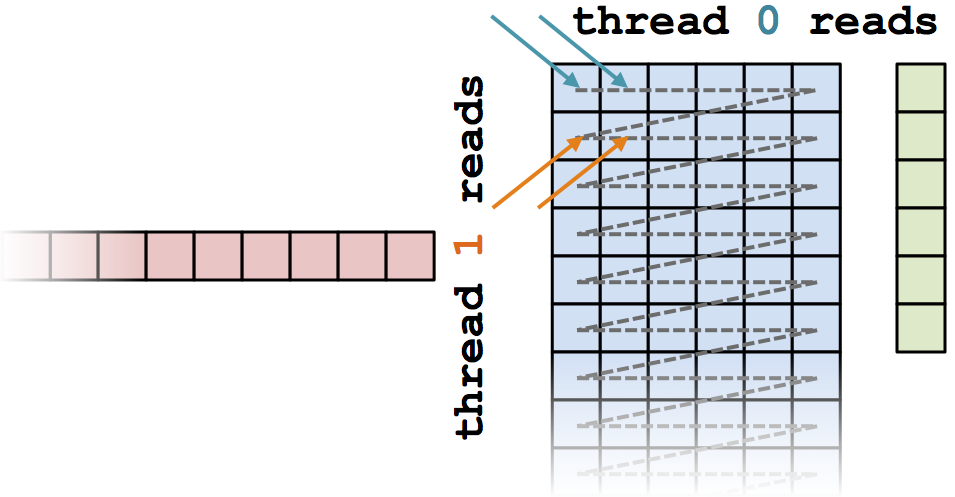
\includegraphics[width=0.65\textwidth]{figures/InnerProductExample_LayoutRight_withThreadReads}
  \end{center}

  \vspace{-28pt}
  \pause

  \begin{itemize}
    \item{\textbf{HostSpace}: cached ({\color{darkgreen}good})}
    \item{\textbf{CudaSpace}: uncoalesced ({\color{red}bad})}
  \end{itemize}

\end{frame}
\fi
\setcounter{subfigure}{0}% Reset subfigure counter


%==========================================================================

\ifmedium
\begin{frame}[fragile]{Example: inner product (3)}

  \begin{block}{Important point}
    Performant memory access is achieved by Kokkos mapping parallel work indices \textbf{and} multidimensional array layout \emph{optimally for the architecture}.
  \end{block}

  \vspace{3pt}

  \ul{\textbf{Analysis: column-major} (\texttt{LayoutLeft})}

  \vspace{-10pt}

  \begin{center}
    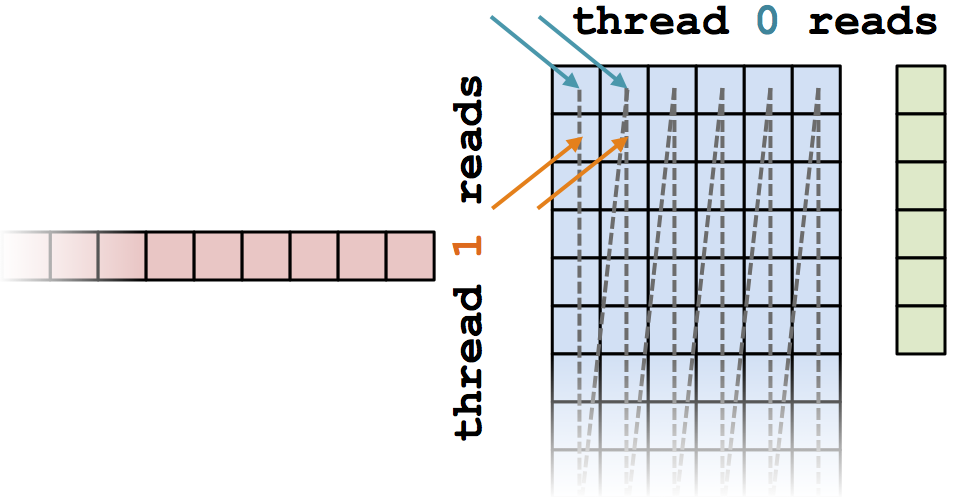
\includegraphics[width=0.65\textwidth]{figures/InnerProductExample_LayoutLeft_withThreadReads}
  \end{center}

  \vspace{-28pt}
  \pause

  \begin{itemize}
    \item{\textbf{HostSpace}: uncached ({\color{red}bad})}
    \item{\textbf{CudaSpace}: coalesced ({\color{darkgreen}good})}
  \end{itemize}

\end{frame}
\fi
\setcounter{subfigure}{0}% Reset subfigure counter

%==========================================================================

\begin{frame}[fragile]{Example: inner product (4)}

  \ul{\textbf{Analysis: Kokkos architecture-dependent}}

  \vspace{-3pt}

  \begin{code}[keywords={}]
View<double**, @boldExecutionSpace@bold> @blueA@blue(N, M);
parallel_for(RangePolicy< @boldExecutionSpace@bold>(0, N),
  ... thisRowsSum += @blueA@blue(j, i) * @darkgreenx@darkgreen(i);
  \end{code}

  \vspace{-20pt}

  \begin{figure}
    \centering
    \subfloat[\texttt{OpenMP}]{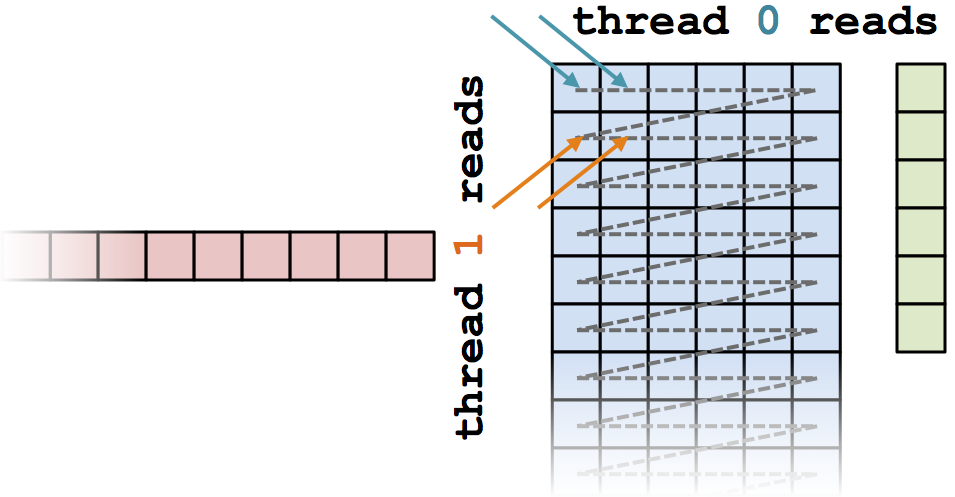
\includegraphics[trim=450pt 0pt 0pt 0pt, clip,width=0.30\textwidth]{figures/InnerProductExample_LayoutRight_withThreadReads}} \qquad
    \subfloat[\texttt{Cuda}]{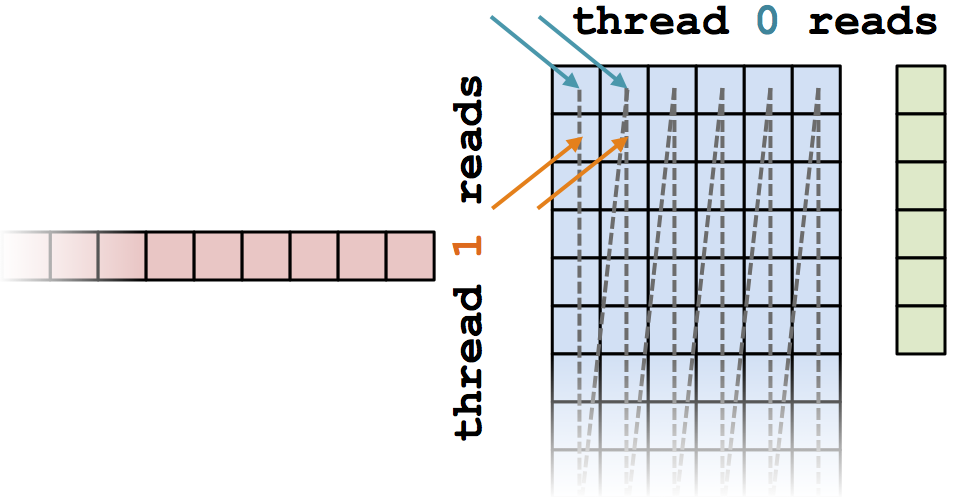
\includegraphics[trim=450pt 0pt 0pt 0pt, clip,width=0.30\textwidth]{figures/InnerProductExample_LayoutLeft_withThreadReads}}
  \end{figure}

  \vspace{-10pt}

  \begin{itemize}
    \item{\textbf{HostSpace}: cached ({\color{darkgreen}good})}
    \item{\textbf{CudaSpace}: coalesced ({\color{darkgreen}good})}
  \end{itemize}

\end{frame}
\setcounter{subfigure}{0}% Reset subfigure counter

%==========================================================================

\begin{frame}[fragile]{Example: inner product (5)}

  \vspace{-10pt}

    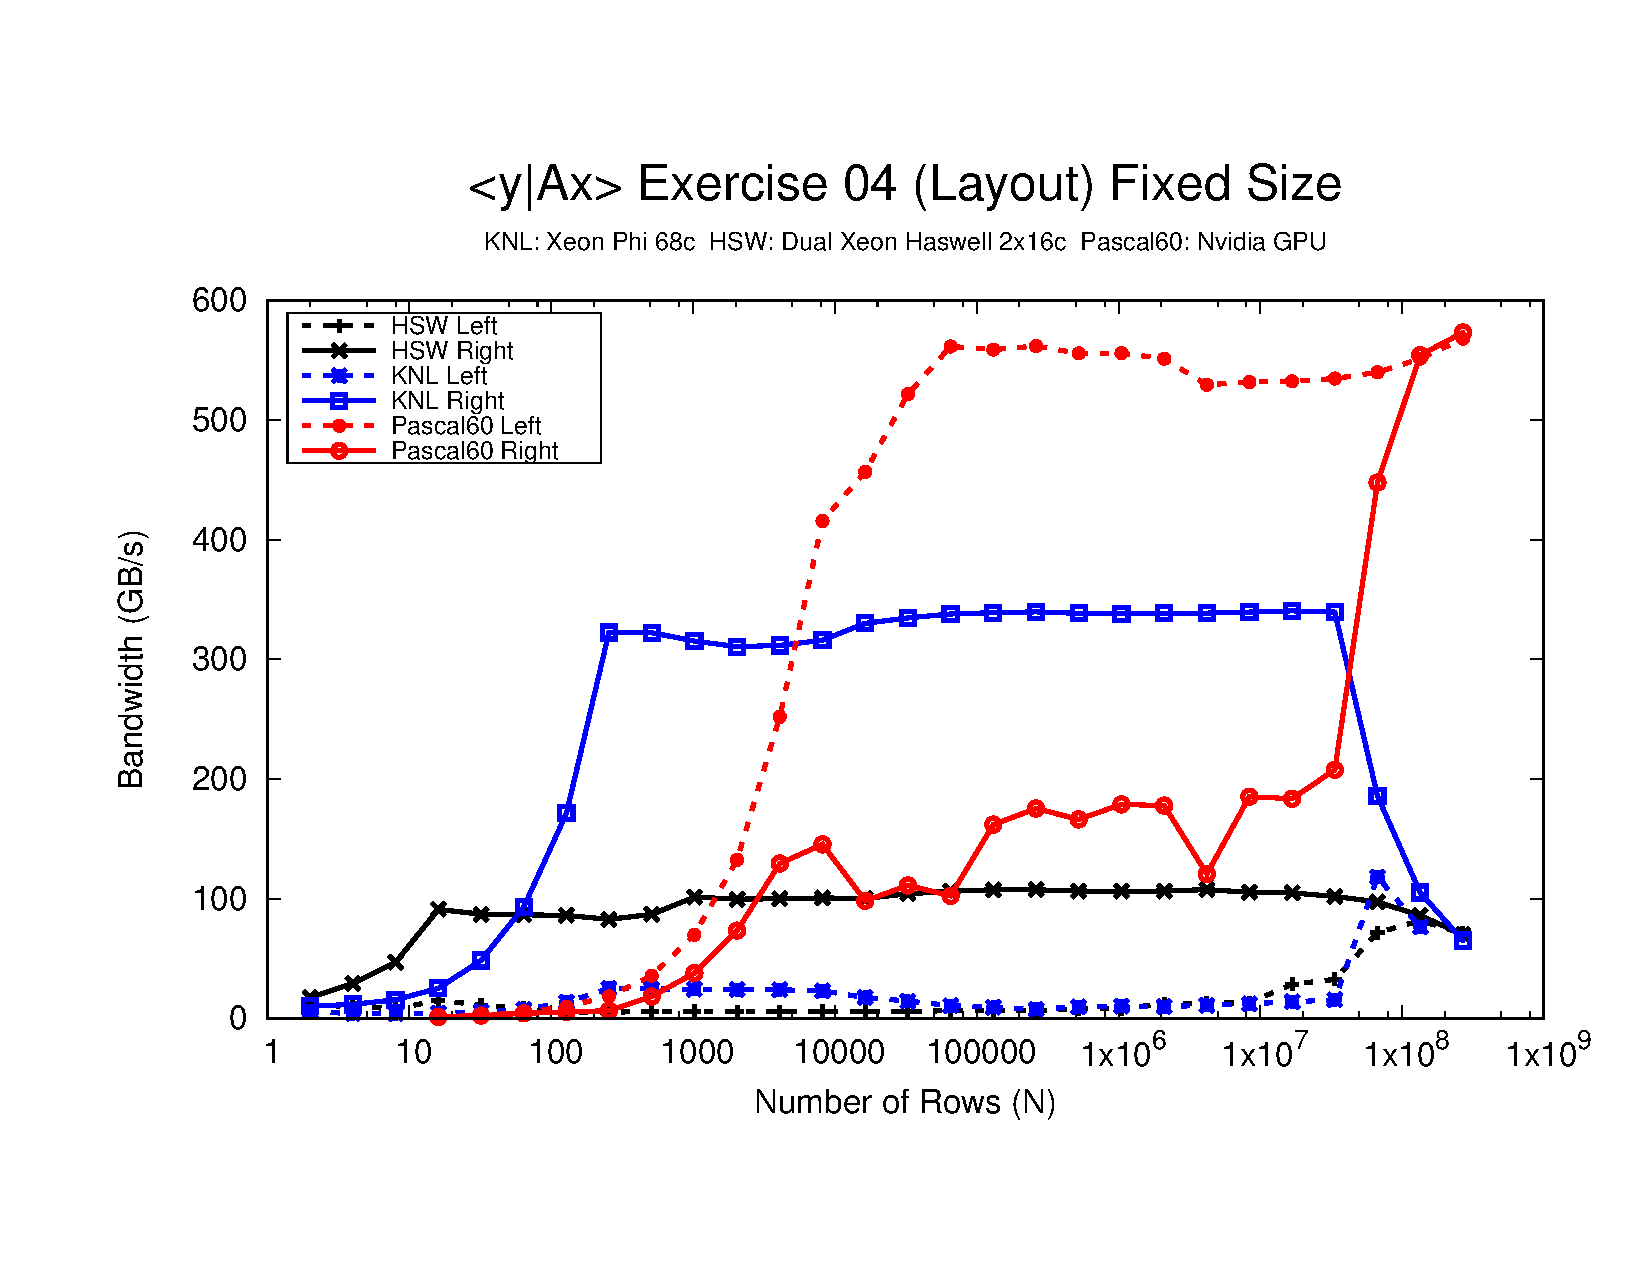
\includegraphics[viewport=1.25in 3.0in 10in 6in, width=0.95\textwidth]{figures/Exercise04-Performance.pdf}

  \vspace{-15pt}

  \begin{textblock*}{0.5\textwidth}(0.65\textwidth,0.28\textheight)
    \textbf{coalesced}
  \end{textblock*}

  \begin{textblock*}{0.5\textwidth}(0.60\textwidth,0.44\textheight)
    \textbf{cached}
  \end{textblock*}

  \begin{textblock*}{0.5\textwidth}(0.60\textwidth,0.61\textheight)
    \textbf{uncoalesced}
  \end{textblock*}

  \begin{textblock*}{0.5\textwidth}(0.70\textwidth,0.72\textheight)
    \textbf{cached}
  \end{textblock*}

  \begin{textblock*}{0.5\textwidth}(0.70\textwidth,0.77\textheight)
    \textbf{uncached}
  \end{textblock*}

\end{frame}

%==========================================================================

\begin{frame}{Memory Access Pattern Summary}

  \begin{itemize}
    \item{Every \texttt{View} has a \texttt{Layout} set at compile-time through a \textbf{template parameter}.}
    \item{\texttt{LayoutRight} and \texttt{LayoutLeft} are \textbf{most common}.}
    \item{\texttt{Views} in \texttt{HostSpace} default to \texttt{LayoutRight} and \texttt{Views} in \texttt{CudaSpace} default to \texttt{LayoutLeft}.}
    \item{Layouts are \textbf{extensible} and \textbf{flexible}.}
    %\item{Correct memory access pattern is \textbf{essential} for performance.}
    \item{For performance, memory access patterns must result in \textbf{caching} on a CPU and \textbf{coalescing} on a GPU.}
    \item{Kokkos maps parallel work indices \textit{and} multidimensional array layout for \textbf{performance portable memory access patterns}.}
    \item{There is \textbf{nothing in} \texttt{OpenMP}, \texttt{OpenACC}, or \texttt{OpenCL} to manage layouts.}\\
    $\Rightarrow$ You'll need multiple versions of code or pay the performance penalty.
  \end{itemize}

\end{frame}



\begin{frame}[fragile]{}

  {\Huge Advanced Reductions}

  \vspace{20pt}

  \textbf{Learning objectives:}
  \begin{itemize}
    \item{How to use Reducers to perform different reductions.}
    \item{How to do multiple reductions in one kernel.}
    \item{Using \texttt{Kokkos::View}'s as result for asynchronicity.}
    \item{Custom reductions}
  \end{itemize}

  \vspace{-20pt}

\end{frame}

\begin{frame}[fragile]{Reducers}

\textbf{So far only "sum" reduction. What about other things?}

\textbf{Using a Reducer:}
\begin{code}[linebackgroundcolor={
          \btLstHL<2>{5}{red!20}
        }, keywords={parallel_reduce,double,Max}]
double max_value = 0;
parallel_reduce("Label", numberOfIntervals,
  KOKKOS_LAMBDA(const int64_t i, double & valueToUpdate) {
    double my_value = function(...);
    if(my_value > valueToUpdate) valueToUpdate = my_value;
}, Kokkos::Max<double>(max_value));
\end{code}

\begin{itemize}
\item<2-> Note how the operation in the body matches the reducer op!
\item<3-> The scalar type is used as a template argument.
\item<4-> Many reducers available: \texttt{Sum, Prod, Min, Max, MinLoc,} see:  {\tiny \url{https://kokkos.github.io/kokkos-core-wiki/API/core/builtin_reducers.html}}
\item<5-> Some reducers (like \texttt{MinLoc}) use special scalar types!
\item<6-> Custom value types supported via specialization of \texttt{reduction\_identity}.
\end{itemize}
\end{frame}

\begin{frame}[fragile]{Simultaneous Reductions}

\textbf{Sometimes multiple reductions are needed}

	\begin{itemize}
		\item Provide multiple reducers/result arguments
		\item Functor/Lambda operator takes matching thread-local variables
		\item Mixing scalar types is fine.
	\end{itemize}

\begin{code}[keywords={parallel_reduce,double,float,Max}]
float max_value = 0;
double sum = 0;
parallel_reduce("Label", numberOfIntervals,
    KOKKOS_LAMBDA(const int64_t i,float& tl_max,double& tl_sum){
  float a_i = a[i];
  if(a_i > tl_max) tl_max = a_i;
  tl_sum += a_i;
}, Kokkos::Max<float>(max_value),sum);
\end{code}

\end{frame}

\begin{frame}[fragile]{Views as Result arguments}

\textbf{Reducing into a Scalar is blocking!}

	\begin{itemize}
		\item Providing a reference to scalar means no lifetime expectation.
			\begin{itemize}
				\item Call to \texttt{parallel\_reduce} returns after writing the result.
			\end{itemize}
		\item \texttt{Kokkos::View} can be used as a result, allowing for potentially non-blocking execution.
		\item Can provide \texttt{View} to host memory, or to memory accessible by the \texttt{ExecutionSpace} for the reduction.
		\item Works with Reducers too!
	\end{itemize}

	\begin{code}[keywords={parallel_reduce,double,View,RangePolicy,CudaSpace,HostSpace}]
View<double,HostSpace> h_sum("sum_h");
View<double,CudaSpace> d_sum("sum_d");
using policy_t = RangePolicy<Cuda>;

parallel_reduce("Label", policy_t(0,N), SomeFunctor, 
  h_sum);

parallel_reduce("Label", policy_t(0,N), SomeFunctor, 
  Kokkos::Sum<double,CudaSpace>(d_sum));
\end{code}
\end{frame}

\begin{frame}[fragile]{Custom Reductions}
\textbf{Pseudocode for Kokkos implementation}
\begin{code}[keywords={parallel_reduce,custom}]
per_thread:
  value& tmp=init(local_tmp);
  for (i in local range)
    functor(i, tmp)
call join for merging values between threads
  in the same thread group
let one (the last) thread group merge all results
  from all thread groups
call final(result) on one thread 
\end{code}

Three ingredients
\begin{itemize}
\item init (optional), default: default constructor
\item join (required)
\item final (optional), default: no-op
\end{itemize}

\end{frame}

\begin{frame}[fragile]{Custom Reductions}
Rules for choosing reduction behavior
\begin{enumerate}
\item If a reducer is specified (return type is a functor with \texttt{reducer} alias to itself), use that.
\item If functor implements \texttt{join}, use functor as reducer.
\item Otherwise, assume \texttt{join} behaves like \texttt{operator+}.
\end{enumerate}

Note that the functor's \texttt{init}, \texttt{join}, \texttt{final} members must be tagged if the call operator is tagged. The reducers member functions must never be tagged.
\end{frame}

\begin{frame}[fragile]{Reducer Concept}
\scriptsize
\begin{code}[basicstyle=\tiny]
class Reducer {
  public:
    using reducer    = Reducer;
    using value_type = ... ;
    using result_view_type = Kokkos::View<value_type, ... >;

    KOKKOS_FUNCTION
    void join(value_type& dest, const value_type& src) const;

    //optional
    KOKKOS_INLINE_FUNCTION
    void init(value_type& val) const;
   
    //optional
    KOKKOS_INLINE_FUNCTION
    void final(value_type& val) const;

    KOKKOS_INLINE_FUNCTION
    value_type& reference() const;

    KOKKOS_INLINE_FUNCTION
    result_view_type view() const;

    KOKKOS_INLINE_FUNCTION
    Reducer(value_type& value_);

    KOKKOS_INLINE_FUNCTION
    Reducer(const result_view_type& value_);
};
\end{code}
\end{frame}


\begin{frame}[fragile]{Subviews}

  {\Huge Subviews: Taking slices of Views}

  \vspace{20pt}

  \textbf{Learning objectives:}
  \begin{itemize}
    \item{Introduce Kokkos::subview---basic capabilities and syntax}
    \item{Suggested usage and practices}
    \item{View assignment rules}
  \end{itemize}

  \vspace{-20pt}

\end{frame}

%==========================================================================

\begin{frame}[fragile]{Subviews: Motivation}

  Sometimes you have to call functions on a subset of data:

  \vspace{5pt}

  \pause
  Example: call a frobenius norm on a matrix slice of a rank-3 tensor:
  \begin{code}[]
double special_norm(View<double***> tensor, int i) {

  auto matrix = ???;
  // Call a function that takes a matrix:
  return some_library::frobenius_norm(matrix);
}
    \end{code}
    \pause

    In Fortran or Matlab or Python you can get such a slice:

    \begin{code}
    tensor(i,:,:)
    \end{code}

    \pause
    Kokkos can do that too!
    \begin{block}{Subview}
     \texttt{Kokkos::subview} can be used to get a view to a subset of an existing \texttt{View}.
     \end{block}

\end{frame}


%==========================================================================

\begin{frame}[fragile]{Subviews (1)}

  \textbf{Subview description:}

  \vspace{5pt}

  \begin{itemize}
    \item{A subview is a ``slice'' of a View}
    \pause
    \begin{itemize}
      \item{The function template \texttt{Kokkos::subview()} takes a \texttt{View} and a slice for each dimension and returns a \texttt{View} of the appropriate shape.}
      \pause
      \item{The subview and original View point to the same data---no extra memory allocation nor copying}        
    \end{itemize}
    \pause
    \item{Can be constructed on host or within a kernel, since no allocation of memory occurs}
    \pause
    \item{Similar capability as provided by Matlab, Fortran, Python, etc., using ``colon'' notation}
  \end{itemize}

\end{frame}

%==========================================================================

\begin{frame}[fragile]{Subviews (2)}

  \textbf{Introductory Usage Demo:}

  \vspace{5pt}

  {Given a \texttt{View}:}

  \lstset{mathescape, escapeinside={<@}{@>},
          language=C,
          keywords={}}

  \begin{lstlisting}
    Kokkos::View<double***> v("v", N0, N1, N2);
  \end{lstlisting}
  
  \pause

  {Say we want a 2-dimensional slice at an index \texttt{i0} in the first dimension---that is, in Matlab/Fortran/Python notation:}
  \begin{lstlisting}
    slicei0 = v(i0, :, :);
  \end{lstlisting}

  \pause
  {This can be accomplished in Kokkos using a subview as follows:}
  \begin{lstlisting}
    auto sv_i0 = 
      Kokkos::subview(v, i0, Kokkos::ALL, Kokkos::ALL);

    // Just like in Python, you can do the same thing with
    // the equivalent of v(i0, 0:N1, 0:N2)
    auto sv_i0_other = 
      Kokkos::subview(v, i0, Kokkos::make_pair(0, N1),
                             Kokkos::make_pair(0, N2));
  \end{lstlisting}

\end{frame}


%==========================================================================

\begin{frame}[fragile]{Subviews (3)}

\textbf{Subview can take three types of slice arguments:}

\begin{itemize}
\item \textbf{Index}
\begin{itemize}
  \item For every index $i$ the rank of the resulting \texttt{View} is decreased by one.
  \item Must be between $0<=i<extent(dim)$
\end{itemize}
\item \textbf{Kokkos::pair}
\begin{itemize}
  \item References a half-open range of indices.
  \item The begin and end must be within the extents of the original view. 
\end{itemize}
\item \textbf{Kokkos::ALL}
\begin{itemize}
  \item References the entire extent in that dimension.
  \item Equivalent to providing \texttt{make\_pair(0,v.extent(dim))}
\end{itemize}
\end{itemize}

\end{frame}

\begin{frame}[fragile]{Subviews (4)}

  \textbf{Usage notes:}

  %\vspace{5pt}

  \begin{itemize}
    \item{Use \texttt{auto} for the type of a subview (unless you can't)}
      \pause
  \begin{itemize}
      \pause
    \item{The return type of \texttt{Kokkos::subview()} is implementation defined for performance reasons}
      \pause
    \item{You can also use \texttt{decltype(subview(/*...*/))} if you really need to spell name of the type somewhere}
  \end{itemize}
      \pause
    \item{Use \texttt{Kokkos::pair} for partial ranges if subview created within a kernel}
      \pause
    \item{Constructing subviews in inner loop code can have performance implications (for now\dots)}
      \pause
    \begin{itemize}
      \item{This will likely be far less of an issue in the future.}
      \pause
      \item{Prioritize readability and maintainability first, then make changes only if you see a performance impact.}
      \pause
    \end{itemize}
  \end{itemize}

\end{frame}

%==========================================================================

\begin{frame}[fragile]{Exercise---Subviews: Basic usage}

  \textbf{Details}:
  \begin{small}
  \begin{itemize}
    \item Location: \ExerciseDirectory{subview/Begin}
    \item This begins with the \texttt{Solution} of 04
    \item In the parallel reduce kernel, create a subview for row j of view A
    \item Use this subview when computing A(j,:)*x(:) rather than the matrix A
  \end{itemize}
  \end{small}

\begin{code}
  # Compile for CPU
  cmake -B build_openmp -DKokkos_ENABLE_OPENMP=ON
  cmake --build build_openmp
  # Run on CPU
  ./build_openmp/subview_exercise -S 26
  # Note the warnings, set appropriate environment variables
  # Compile for GPU
  cmake -B build_cuda -DKokkos_ENABLE_CUDA=ON
  cmake --build build_cuda
  # Run on GPU
  ./build_cuda/subview_exercise -S 26
\end{code}

\end{frame}

%==========================================================================

\begin{frame}[fragile]{Aside: View Assignment (1)}

  \textbf{\texttt{View::operator=()} just does the ``Right Thing''\textsuperscript{TM}}

  \vspace{5pt}

  \begin{itemize}
    \item{\texttt{View<int**> a; a = View<int*[5]>("b", 4)}}
    \pause
    {\color{darkgreen}{$=>$ Okay}}
    \pause
    \item{\texttt{View<int*[5]> a; a = View<int**>("b", 4, 5)}}\\
    \pause
    {\color{darkgreen}{$=>$ Okay, checked at runtime}}
    \pause
    \item{\texttt{View<int*[5]> a; a = View<int*[3]>("b", 4)}}\\
    \pause
    {\color{darkred}{$=>$ Compilation error}}
    \pause
    \item{\texttt{View<int*[5]> a; a = View<int**>("b", 4, 3)}}\\
    \pause
    {\color{darkred}{$=>$ Runtime error}}
    \pause
    \item{\texttt{View<int*, CudaSpace> a;}\\
    \texttt{a = View<int*, HostSpace>("b", 4)}}\\
    \pause
    {\color{darkred}{$=>$ Compilation error}}
    \item{\texttt{View<int**, LayoutLeft> a;}\\
    \texttt{a = View<int**, LayoutRight>("b", 4, 5)}}\\
    \pause
    {\color{darkred}{$=>$ Compilation error}}
  \end{itemize}

\end{frame}

%==========================================================================

\begin{frame}[fragile]{Aside: View Assignment (2)}

  \textbf{\texttt{View::operator=()} just does the ``Right Thing''\textsuperscript{TM}}

  \vspace{5pt}

  \begin{itemize}
    \item{\texttt{View<const int*> a; a = View<int*>("b", 4)}}\\
    \pause
    {\color{darkgreen}{$=>$ Okay}}
    \pause
    \item{\texttt{View<int*> a; a = View<const int*>("b", 4)}}\\
    \pause
    {\color{darkred}{$=>$ Compilation error}}
    \pause
    \item{\texttt{View<int*[5], LayoutStride> a;}\\ \texttt{a = View<int*[5], LayoutLeft>("b", 4)}}
    \pause
    {\color{darkgreen}{$=>$ Okay, converting compile-time strides into runtime strides}}
    \pause
    \item{\texttt{View<int*[5], LayoutLeft> a;}\\ \texttt{a = View<int*[5], LayoutStride>("b", 4)}}
    \pause
    {\color{yellow!50!black}{$=>$ Okay, but only if strides match layout left (checked at runtime)}}
  \end{itemize}

\end{frame}
%==========================================================================

\begin{frame}[fragile]{View Assignment: subview}

  {Given a \texttt{View}:}
  \vspace{-2pt}

  \lstset{mathescape, escapeinside={<@}{@>},
          language=C,
          keywords={}}

  \begin{lstlisting}
    Kokkos::View<int***> v("v", n0, n1, n2);
  \end{lstlisting}
  \vspace{-5pt}
  \begin{itemize}
    \item{\texttt{View<int***> a;}\\
    \texttt{a = Kokkos::subview(v, ALL, 42, ALL);}}\\
    \pause
    {\color{darkred}{$=>$ Compilation error}}
    \pause
    \item{\texttt{View<int*> a;}\\
    \texttt{a = Kokkos::subview(v, ALL, 5, 42);}}\\
    \pause
    {\color{darkgreen}{$=>$ Okay for LayoutLeft}} but {\color{darkred}{$=>$ Compilation error for LayoutRight}}
    \pause
    \item{\texttt{View<int**> a;}\\
    \texttt{a = Kokkos::subview(v, ALL, 15, ALL);}}\\
    \pause
    {\color{darkred}{$=>$ Runtime error (!)}}
    \pause
    \item{\texttt{View<int**, LayoutStride> a;}\\
    \texttt{a = Kokkos::subview(v, ALL, 15, ALL);}}\\
    \pause
    {\color{darkgreen}{$=>$ Okay}}
  \end{itemize}

\end{frame}

%==========================================================================

\begin{frame}[fragile]{Subview Summary}

  \begin{itemize}
    \item Use subviews to get a portion of a \texttt{View}. Helps with:
	    \begin{itemize}
           \item code reuse
	   \item code readability
	   \item library function compatibility
	    \end{itemize}
    \pause
    \item Kokkos supports slicing Views similar to Python/Matlab/Fortran slicing syntax 
	\begin{code}[]
auto sv = Kokkos::subview(v, 42, ALL, std::make_pair(3, 17));
	\end{code}
    \pause
    \item The return type of \texttt{subview} is complicated. Use \textbf{auto}!!
    \item {\texttt{View::operator=()} just does the ``Right Thing''\textsuperscript{TM}}
      \begin{itemize}
         \item So generally don't worry about it at first! This is advanced stuff, and more for future reference.
      \end{itemize}
  \end{itemize}

\end{frame}


\begin{frame}[fragile]{MDRangePolicy}

  {\Huge Tightly Nested Loops with MDRangePolicy}

  \vspace{20pt}

  \textbf{Learning objectives:}
  \begin{itemize}
    \item{Demonstrate usage of the MDRangePolicy with tightly nested loops.}
    \item{Syntax - Required and optional settings}
    \item{Code demo and example}
  \end{itemize}

  \vspace{-20pt}

\end{frame}

%==========================================================================

\begin{frame}[fragile]{MDRangePolicy (0)}

  \textbf{Motivating example}: Consider the nested for loops:

%  \vspace{5pt}

  \lstset{mathescape, escapeinside={<@}{@>},
          language=C,
          keywords={}}

  \begin{lstlisting}%[linebackgroundcolor={
    %    \btLstHL{1-3}{darkred!20}
    %  }
    %]

  for ( int i = 0; i < N0; ++i )
  for ( int j = 0; j < N1; ++j )
  for ( int k = 0; k < N2; ++k )
    some_init_fcn(i, j, k);

  \end{lstlisting}

%  \vspace{-11pt}

%  \begin{itemize}
%    \item{Based on Kokkos lessons thus far, you might parallelize this as follows:}
%  \end{itemize}

  {Based on Kokkos lessons thus far, you might parallelize this as}


  \begin{lstlisting}%[linebackgroundcolor={
    %    \btLstHL{3-4}{bodyColor}
    %  }
    %]

  Kokkos::parallel_for("Label", N0,
                       KOKKOS_LAMBDA (const i) {
                         for ( int j = 0; j < N1; ++j )
                         for ( int k = 0; k < N2; ++k )
                          some_init_fcn(i, j, k);
                       }
                       );
  \end{lstlisting}

%  \begin{textblock*}{0.5\textwidth}(0.08\textwidth,0.235\textheight)
%    \rotatebox{90}{{\footnotesize {\color{darkred!80} section 1}}}
%  \end{textblock*}

%  \begin{textblock*}{0.5\textwidth}(0.08\textwidth,0.40\textheight)
%    \rotatebox{90}{{\footnotesize {\color{blue!80} section 2}}}
%  \end{textblock*}

%  \pause

  \vspace{-5pt}

  \begin{itemize}
    \item{\small{This only parallelizes along one dimension, leaving potential parallelism unexploited.}}
    \item{\small{What if Ni is too small to amortize the cost of constructing a parallel region, but Ni*Nj*Nk makes it worthwhile?}}
  \end{itemize}

%  \begin{itemize}
%    \item{Where will {\color{darkred!80}section 1} be run?  CPU?  GPU?}
%    \item{Where will {\color{blue!80}section 2} be run?  CPU?  GPU?}
%    \item{How do I \textbf{control} where code is executed?}
%  \end{itemize}

%  \pause
%  \vspace{5pt}

%  \hspace{20pt}{\Large $\Rightarrow$ \textbf{Execution spaces}}

\end{frame}

%==========================================================================

\begin{frame}[fragile]{MDRangePolicy (1)}
   \textbf{OpenMP has a solution: the collapse clause}

  \begin{code}[linebackgroundcolor={
        \btLstHL<1->{5}{bodyColor}
      },
      frame=single
    ]
#pragma @policyomp parallel@policy @patternfor@pattern @policycollapse(3)@policy
@patternfor@pattern (int64_t i = @policy0; i < N0@policy; ++i) {
  @patternfor@pattern (int64_t j = @policy0; j < N1@policy; ++j) {
    @patternfor@pattern (int64_t k = @policy0; k < N2@policy; ++k) {
      /* loop body */
    }
  }
}
  \end{code}

  \pause

Note this changed the policy by adding a `collapse` clause.

\pause

	\vspace{0.5cm}

	\textbf{With Kokkos you also change the policy:}

  \begin{code}[linebackgroundcolor={
        \btLstHL<1->{3}{bodyColor}
      },
      frame=single
    ]
@patternparallel_for@pattern("L", @policyMDRangePolicy<Rank<3>>({0,0,0},{N0,N1,N2})@policy, 
   KOKKOS_LAMBDA(int64_t i, int64_t j, int64_t k) {
     /* loop body */
});
  \end{code}

\end{frame}

\begin{frame}[fragile]{MDRangePolicy (2)}

\begin{block}{MDRangePolicy}
   MDRangePolicy can parallelize tightly nested loops of 2 to 6 dimensions.
\end{block}

	\vspace{0.5cm}

  \begin{code}[linebackgroundcolor={
        \btLstHL<1->{3}{bodyColor}
      },
      frame=single
    ]
@patternparallel_for@pattern("L", @policyMDRangePolicy<Rank<3>>({0,0,0},{N0,N1,N2})@policy, 
   KOKKOS_LAMBDA(int64_t i, int64_t j, int64_t k) {
     /* loop body */
});
  \end{code}

\begin{itemize}
   \item<2-> Specify the dimensionality of the loop with $Rank<DIM>$.
   \item<3-> As with Kokkos Views: only rectangular iteration spaces.
   \item<4-> Provide initializer lists for begin and end values.
   \item<5-> The functor/lambda takes matching number of indicies. 
\end{itemize}
\end{frame}

\begin{frame}[fragile]{MDRangePolicy (3)}
   \textbf{You can also do Reductions:}

  \begin{code}[linebackgroundcolor={
        \btLstHL<1->{5-6}{bodyColor}
      },
      frame=single
    ]
double result;
@patternparallel_reduce@pattern("Label", 
  @policyMDRangePolicy<Rank<3>>({0,0,0},{N0,N1,N2})@policy, 
  KOKKOS_LAMBDA(int i, int j, int k, double& lsum) {
     /* loop body */
  lsum += something;
}, result);
  \end{code}

\begin{itemize}
   \item<2-> The Policy doesn't change the rules for `parallel\_reduce`.
   \item<3-> Additional Thread Local Argument.
   \item<4-> Can do other reductions with reducers.
   \item<5-> Can use `View`s as reduction argument.
   \item<6-> Multiple reducers not yet implemented though.
\end{itemize}
\end{frame}

\begin{frame}[fragile]{MDRangePolicy (4)}
   In structured grid applications a \textbf{tiling} strategy is often used to help with caching.

	\begin{block}{Tiling}
		MDRangePolicy uses a tiling strategy for the iteration space.
	\end{block}

	\begin{itemize}
		\item Specified as a third initializer list.
		\item For GPUs a tile is handled by a single thread block.
			\begin{itemize}
				\item If you provide too large a tile size this will fail!
			\end{itemize}
		\item In Kokkos 3.3 we will add auto tuning for tile sizes. 
	\end{itemize}

\begin{code}[keywords={}]
double result;
parallel_reduce("Label", 
  MDRangePolicy<Rank<3>>({0,0,0},{N0,N1,N2},@policy{T0,T1,T2}@policy), 
  KOKKOS_LAMBDA(int i, int j, int k, double& lsum) {
     /* loop body */
  lsum += something;
}, result);
  \end{code}

\end{frame}


\begin{frame}[fragile]{MDRangePolicy (5)}

  Initializing a Matrix:
  
\begin{code}[keywords={LayoutLeft}]
View<double**,LayoutLeft> A("A",N0,N1);
parallel_for("Label", 
  MDRangePolicy<Rank<2>>({0,0},{N0,N1}), 
  KOKKOS_LAMBDA(int i, int j) {
    A(i,j) = 1000.0 * i + 1.0*j;
});
\end{code}

\begin{code}[keywords={LayoutRight}]
View<double**,LayoutRight> B("B",N0,N1);
parallel_for("Label", 
  MDRangePolicy<Rank<2>>({0,0},{N0,N1}), 
  KOKKOS_LAMBDA(int i, int j) {
    B(i,j) = 1000.0 * i + 1.0*j;
});
\end{code} 

\pause

	\textbf{How do I make sure that I get the right access pattern?}

\end{frame}


\begin{frame}[fragile]{MDRangePolicy (6)}
\begin{block}{Iteration Pattern}
MDRangePolicy provides compile time control over iteration patterns.
\end{block}

  \begin{lstlisting}[basicstyle=\large,gobble=4]
    Kokkos::Rank< N, IterateOuter, IterateInner >
  \end{lstlisting}

  \begin{itemize}
    \item{\small{\textbf{N: (Required)} the rank of the index space (limited from 2 to 6)}}
    \item{\small{\textbf{IterateOuter (Optional)} iteration pattern between tiles}}
    \begin{itemize}
      \item{\small{\textbf{Options:} Iterate::Left, Iterate::Right, Iterate::Default}}
    \end{itemize}
    \item{\small{\textbf{IterateInner (Optional)} iteration pattern within tiles}}
    \begin{itemize}
      \item{\small{\textbf{Options:} Iterate::Left, Iterate::Right, Iterate::Default}}
    \end{itemize}
  \end{itemize}
\end{frame}

%==========================================================================

\begin{frame}[fragile]{MDRangePolicy (7)}

  Initializing a Matrix fast:
  
\begin{code}[keywords={LayoutLeft,Iterate,Left,Right}]
View<double**,LayoutLeft> A("A",N0,N1);
parallel_for("Label", 
  MDRangePolicy<Rank<2,Iterate::Left,Iterate::Left>>(
	{0,0},{N0,N1}), 
  KOKKOS_LAMBDA(int i, int j) {
    A(i,j) = 1000.0 * i + 1.0*j;
});
\end{code}

\begin{code}[keywords={LayoutRight}]
View<double**,LayoutRight> B("B",N0,N1);
parallel_for("Label", 
  MDRangePolicy<Rank<2,Iterate::Right,Iterate::Right>>(
	{0,0},{N0,N1}), 
  KOKKOS_LAMBDA(int i, int j) {
    B(i,j) = 1000.0 * i + 1.0*j;
});
\end{code} 

\pause

	\begin{block}{Default Patterns Match}
Default iteration patterns match the default memory layouts!
	\end{block}
\end{frame}



%==========================================================================

\begin{frame}[fragile]{Exercise - mdrange: Initialize multi-dim views with MDRangePolicy}

  \textbf{Details}:
  \begin{small}
  \begin{itemize}
    \item Location: \ExerciseDirectory{mdrange/Begin}
    \item This begins with the \texttt{Solution} of 02
    \item Initialize the device Views x and y directly on the device using a parallel for and RangePolicy
    \item Initialize the device View matrix A directly on the device using a parallel for and MDRangePolicy
  \end{itemize}
  \end{small}

\begin{code}
  # Compile for CPU
  cmake -B build_openmp -DKokkos_ENABLE_OPENMP=ON
  cmake --build build_openmp
  # Run on CPU
  ./build_openmp/mdrange_exercise -S 26
  # Note the warnings, set appropriate environment variables
  # Compile for GPU
  cmake -B build_cuda -DKokkos_ENABLE_CUDA=ON
  cmake --build build_cuda
  # Run on GPU
  ./build_cuda/mdrange_exercise -S 26
\end{code}

\end{frame}

%==========================================================================

\begin{frame}[fragile]{Common Policy Arguments}

  \textbf{Template Parameters common to ALL policies.}

  \begin{itemize}
     \item \texttt{ExecutionSpace}: control where code executes
     \begin{itemize}
       \item{\small{\textbf{Options:} Serial, OpenMP, Threads, Cuda, HIP, ...}}
     \end{itemize}
     \item \texttt{Schedule$<$Options$>$}: set scheduling policy.
     \begin{itemize}
        \item{\small{\textbf{Options:} Static, Dynamic}}
     \end{itemize}

     \item \texttt{IndexType$<$Options$>$}: control internal indexing type
     \begin{itemize}
       \item{\small{\textbf{Options:} int, long, etc}}
     \end{itemize}

     \item \texttt{WorkTag}: enables multiple operators in one functor
	     \begin{code}[keywords={struct,Tag1,Tag2,void,int}]
struct Foo {
  struct Tag1{}; struct Tag2{};
  KOKKOS_FUNCTION void operator(Tag1, int i) const {...}
  KOKKOS_FUNCTION void operator(Tag2, int i) const {...}
  void run_both(int N) { 
    parallel_for(RangePolicy<Tag1>(0,N),*this);
    parallel_for(RangePolicy<Tag2>(0,N),*this);
  }
});
  \end{code}
  \end{itemize}

\end{frame}

%==========================================================================

\begin{frame}[fragile]{MDRangePolicy Section Summary}

  \textbf{MDRangePolicy}
  \begin{itemize}
    \item{allows for tightly nested loops similar to OpenMP's collapse clause.}
    \item{requires functors/lambdas with as many parameters as its rank is.}
    \item{works with \texttt{parallel\_for} and \texttt{parallel\_reduce}.}
    \item{uses a tiling strategy for the iteration space.}
    \item{provides compile time control over iteration patterns.}
  \end{itemize}

\end{frame}

%==========================================================================


\begin{comment}
try a scan and fill for fill array?
\end{comment}

%==========================================================================

\begin{frame}[fragile]

  {\Huge Hierarchical parallelism}

  \vspace{10pt}

  {\large Finding and exploiting more parallelism in your computations.}

  \vspace{20pt}

  \textbf{Learning objectives:}
  \begin{itemize}
    \item {Similarities and differences between outer and inner levels of parallelism}
    \item {Thread teams (league of teams of threads)}
    \item {Performance improvement with well-coordinated teams}
  \end{itemize}

  \vspace{-20pt}

\end{frame}

%==========================================================================

\begin{frame}[fragile]{Example: inner product (0)}

  \ul{\textbf{(Flat parallel) Kernel:}}

  \vspace{-3pt}

  \begin{code}[keywords={}]
Kokkos::parallel_reduce("yAx",N,
  KOKKOS_LAMBDA (const int row, double & valueToUpdate) {
    double thisRowsSum = 0;
    for (int col = 0; col < M; ++col) {
      thisRowsSum += @blueA@blue(row,col) * @darkgreenx@darkgreen(col);
    }
    valueToUpdate += @darkredy@darkred(row) * thisRowsSum;
  }, @orangeresult@orange);
  \end{code}

 \begin{tikzpicture}[remember picture, overlay]
    \node [shift={(-8.0cm,1.10cm)}]  at (current page.south east)
      {%
      \begin{tikzpicture}[remember picture, overlay]
        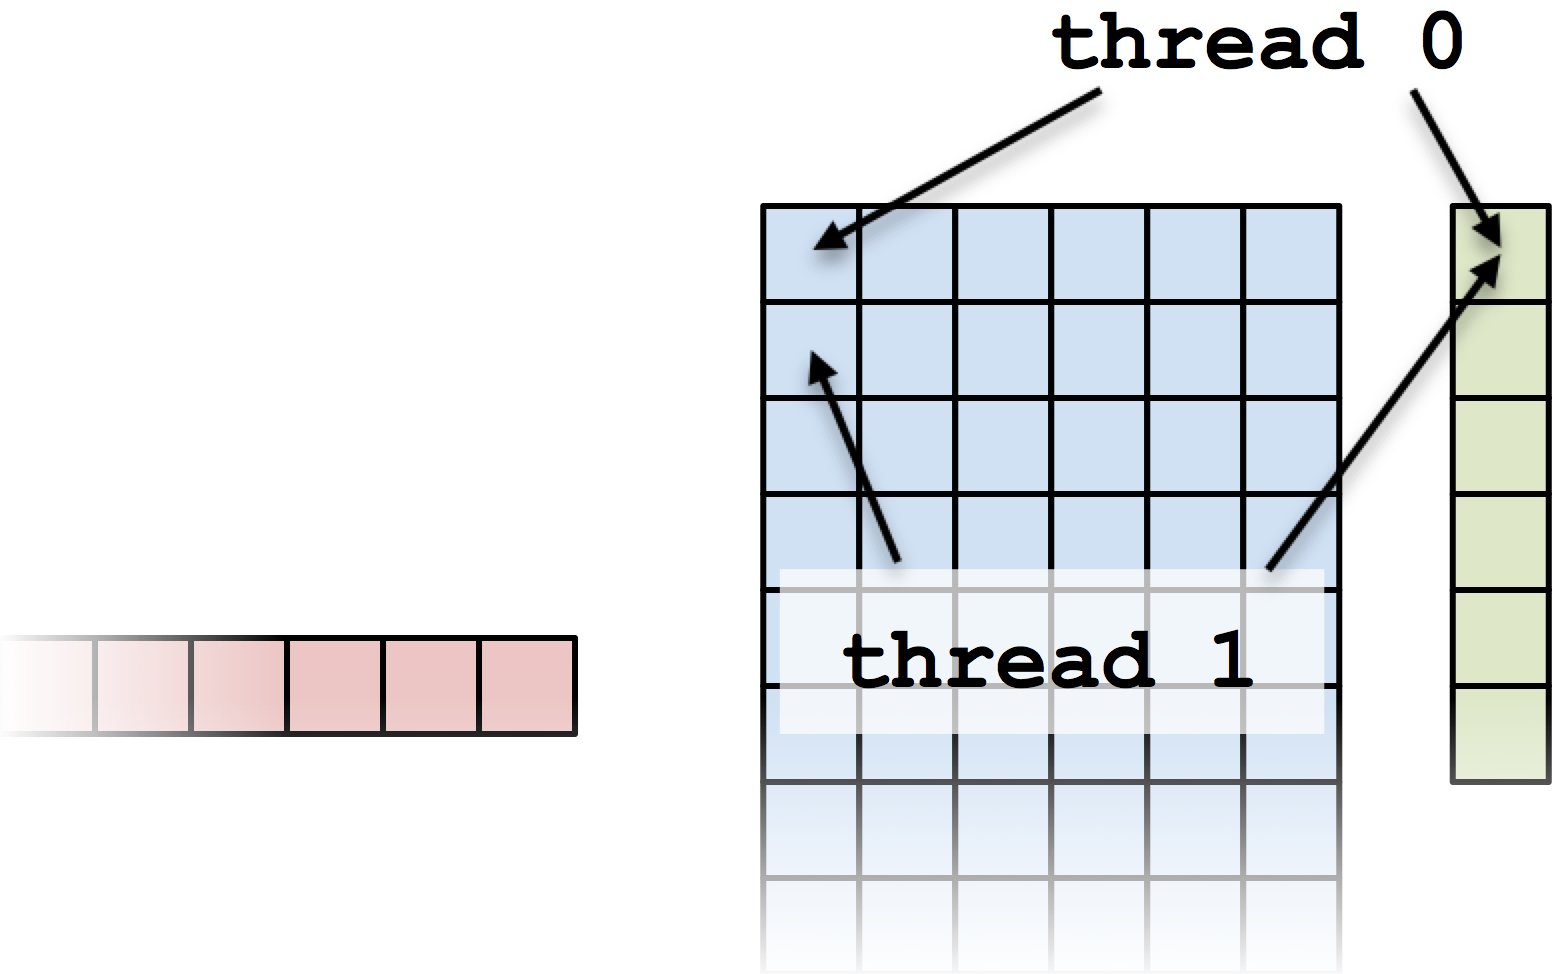
\includegraphics[width=0.60\textwidth]{figures/InnerProductExample_Flat}
      \end{tikzpicture}
      };
  \end{tikzpicture}

  \vspace{10pt}
  \pause

  \begin{columns}[t,onlytextwidth]
    \column{.60\textwidth}
    \textbf{Problem:} What if we don't have enough rows to saturate the GPU?
    \column{.40\textwidth}
  \end{columns}

  \vspace{10pt}
  \pause

  \textbf{Solutions?}
  \pause
  \vspace{-5pt}

  \begin{itemize}
    \item{Atomics}
    \item{Thread teams}
  \end{itemize}

\end{frame}

%==========================================================================
\iffull
\begin{frame}[fragile]{Example: inner product (1)}

  \ul{\textbf{Atomics kernel:}}

  \vspace{-3pt}

  \begin{code}[keywords={}]
Kokkos::parallel_for("yAx", N*M,
  KOKKOS_LAMBDA (const size_t index) {
    const int row = extractRow(index);
    const int col = extractCol(index);
    atomic_add(&@orangeresult@orange, @redy@red(row) * @blueA@blue(row,col) * @darkgreenx@darkgreen(col));
  });
  \end{code}

 \begin{tikzpicture}[remember picture, overlay]
    \node [shift={(-8.0cm,1.10cm)}]  at (current page.south east)
      {%
      \begin{tikzpicture}[remember picture, overlay]
        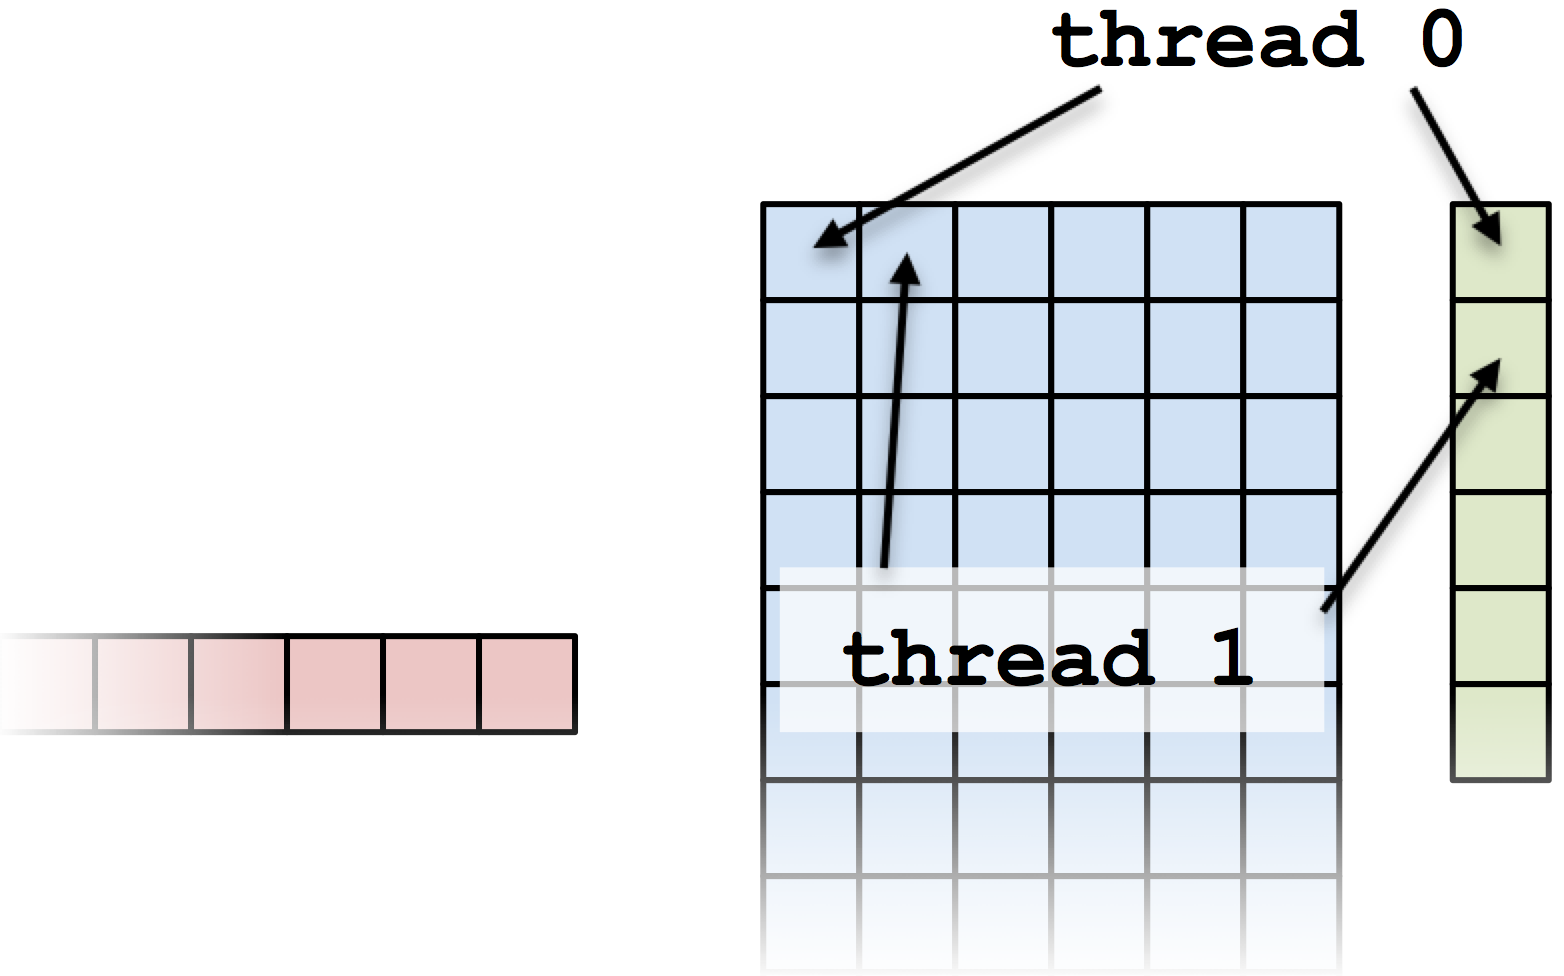
\includegraphics[width=0.60\textwidth]{figures/InnerProductExample_Atomics}
      \end{tikzpicture}
      };
  \end{tikzpicture}

  \vspace{10pt}
  \pause

  \begin{columns}[t,onlytextwidth]
    \column{.60\textwidth}
    {\color{red}\textbf{Problem:}} Poor performance
    \column{.40\textwidth}
  \end{columns}

  \vspace{50pt}

\end{frame}
\fi

%==========================================================================

\begin{frame}[fragile]{Example: inner product (2)}

  Using an atomic with every element is doing scalar integration with atomics.  (See module 3)

  \vspace{10pt}

  Instead, you could envision doing a large number of \texttt{parallel\_reduce} kernels.

  \begin{code}[keywords={}]
for each row
  Functor functor(row, ...);
  parallel_reduce(M, functor);
}
  \end{code}

  \vspace{10pt}
  \pause

  This is an example of \emph{hierarchical work}.

  \begin{block}{Important concept: Hierarchical parallelism}
    Algorithms that exhibit hierarchical structure can exploit hierarchical parallelism with \textbf{thread teams}.
  \end{block}

\end{frame}

%==========================================================================

\ifmedium
\begin{frame}[fragile]{Example: inner product (3)}

  \begin{block}{Important concept: Thread team}
  A collection of threads which are guaranteed to be executing \textbf{concurrently} and \textbf{can synchronize}.
  \end{block}

  \pause
  \vspace{-15pt}

 \begin{tikzpicture}[remember picture, overlay]
    \node [shift={(-6.0cm,0.75cm)}]  at (current page.south east)
      {%
      \begin{tikzpicture}[remember picture, overlay]
        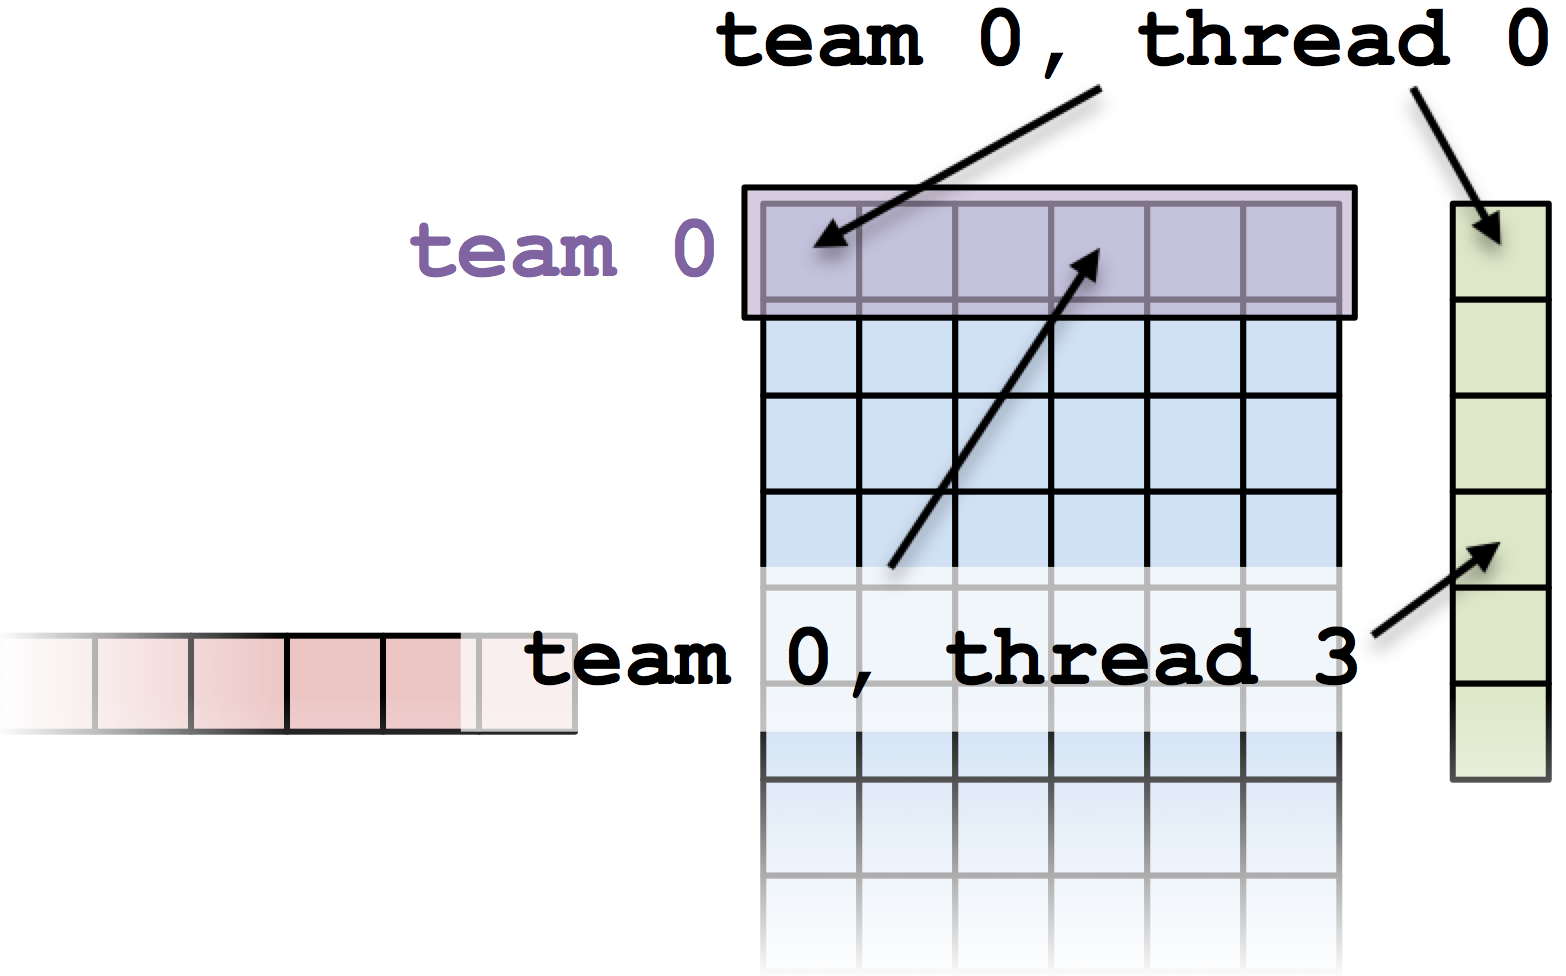
\includegraphics[width=0.53\textwidth]{figures/InnerProductExample_Teams}
      \end{tikzpicture}
      };
  \end{tikzpicture}

  High-level \textbf{strategy}:

  \vspace{-3pt}

  \begin{enumerate}
    \item{Do \textbf{one parallel launch} of \texttt{N} teams.}
    \item{Each team handles a row.}
    \item{The threads within \textbf{teams perform a reduction}.}
    \item{The thread teams \textbf{perform a reduction}.}
  \end{enumerate}

  %\vspace{-15pt}
  \vspace{85pt}

  %\begin{center}
    %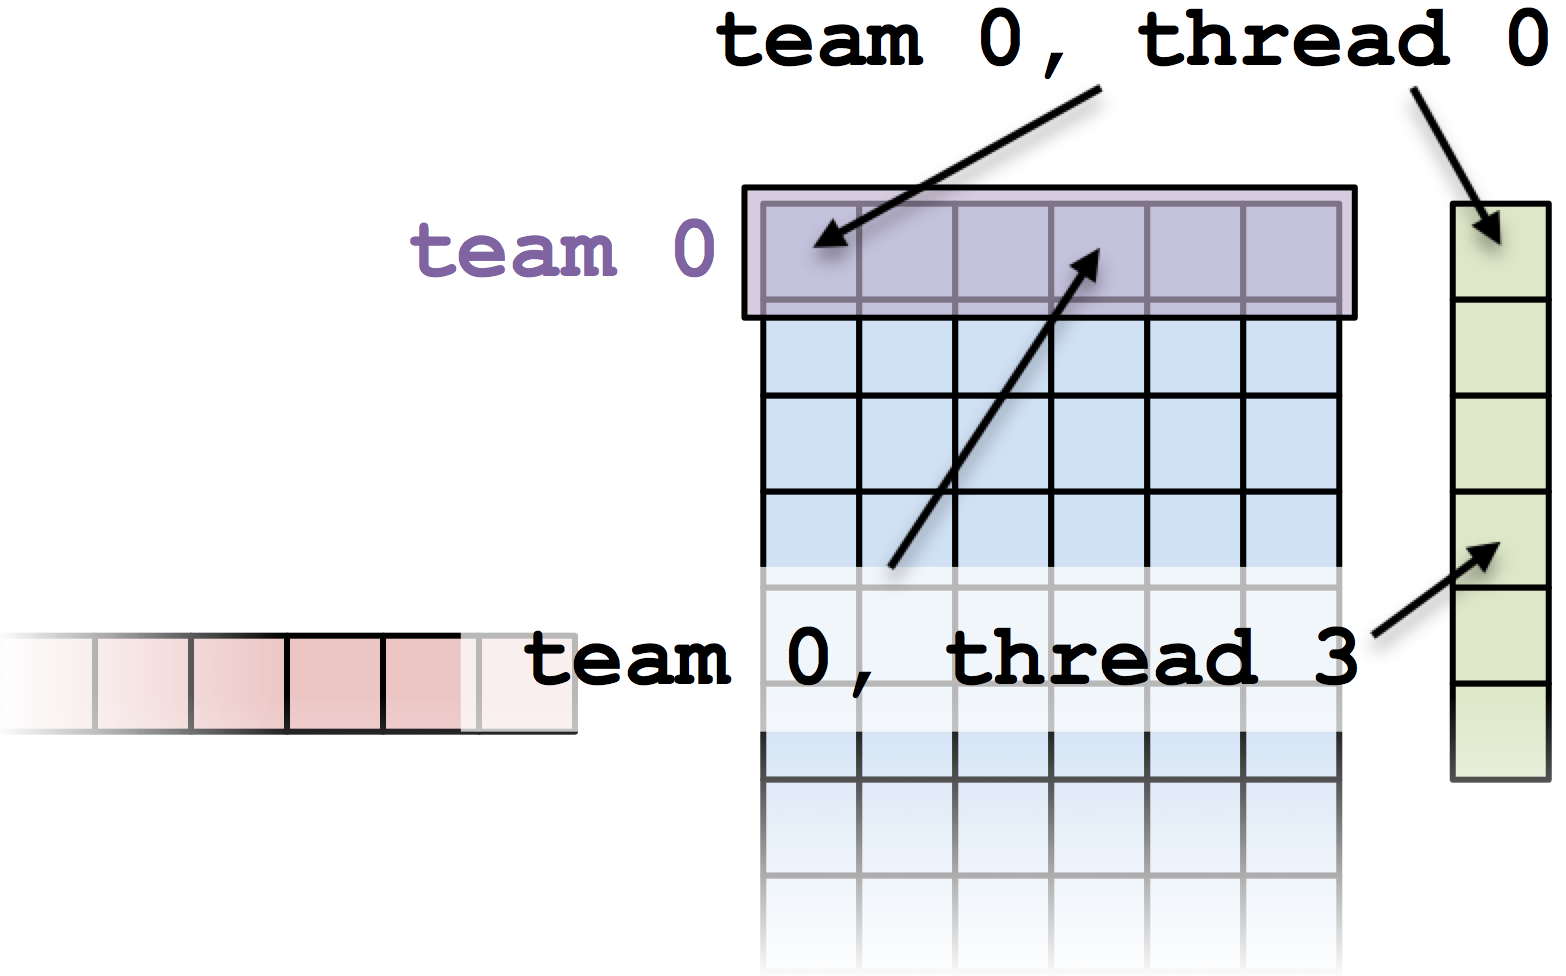
\includegraphics[width=0.40\textwidth]{figures/InnerProductExample_Teams}
  %\end{center}

  %\vspace{-5pt}

\end{frame}
\fi

%==========================================================================

\ifmedium
\begin{frame}[fragile]{Example: inner product (4)}

  \ul{\textbf{The \textit{final} hierarchical parallel kernel:}}

  \begin{code}
parallel_reduce("yAx",
  team_policy(N, Kokkos::AUTO),

  KOKKOS_LAMBDA (const member_type & @blueteamMember@blue, double & @orangeupdate@orange) {
    int @purplerow@purple = @blueteamMember@blue.league_rank();

    double thisRowsSum = 0;
    parallel_reduce(TeamThreadRange(@blueteamMember@blue, M),
      [=] (int @darkgreencol@darkgreen, double & @redinnerUpdate@red) {
        @redinnerUpdate@red += A(@purplerow@purple, @darkgreencol@darkgreen) * x(@darkgreencol@darkgreen);
      }, thisRowsSum);

    if (@blueteamMember@blue.team_rank() == 0) {
      update += y(@purplerow@purple) * thisRowsSum;
    }
  }, @orangeresult@orange);
  \end{code}

  %\vspace{5pt}

  %The \textbf{performance} and \textbf{flexibility} of teams is \emph{naturally} and \emph{concisely} expressed under the Kokkos model.

  %\vspace{1em}

  %Let's walk through how we got to this \textit{final} answer.

\end{frame}
\fi

%==========================================================================

\begin{frame}[fragile]{TeamPolicy (0)}

  \begin{block}{Important point}
    Using teams is changing the execution \emph{policy}.
  \end{block}

  \vspace{10pt}

  ``\textbf{Flat} parallelism'' uses \texttt{RangePolicy}:

  \vspace{3pt}

  \hspace{20pt}We specify a \emph{total amount of work}.

  \vspace{0pt}

  \begin{code}
// total work = N
@patternparallel_for@pattern("Label", 
  @policyRangePolicy<ExecutionSpace>(0,N)@policy, @bodyfunctor@body);
  \end{code}

  \pause
  \vspace{15pt}
  ``\textbf{Hierarchical} parallelism'' uses \texttt{TeamPolicy}:

  \vspace{3pt}

  \hspace{20pt}We specify a \emph{team size} and a \emph{number of teams}.

  \begin{code}[linebackgroundcolor={
      },
      keywords={}
    ]
// total work = numberOfTeams * teamSize
@patternparallel_for@pattern("Label", 
  @policyTeamPolicy<ExecutionSpace>(numberOfTeams, teamSize)@policy, @bodyfunctor@body);
  \end{code}

  \vspace{10pt}
\end{frame}

%==========================================================================

\begin{frame}[fragile]{TeamPolicy (1)}

  \begin{block}{Important point}
    When using teams, functor operators receive a \emph{team member}.
  \end{block}

  \begin{code}[linebackgroundcolor={
      },
      keywords={}
    ]
using member_type = typename TeamPolicy<ExecSpace>::member_type;

void operator()(const member_type & teamMember) {
  <@{\bf // How many teams are there?}@>
  const unsigned int league_size = teamMember.league_size();

  <@{\bf // Which team am I on?}@>
  const unsigned int league_rank = teamMember.league_rank();

  <@{\bf // How many threads are in the team?}@>
  const unsigned int team_size = teamMember.team_size();

  <@{\bf // Which thread am I on this team?}@>
  const unsigned int team_rank = teamMember.team_rank();

  <@{\bf // Make threads in a team wait on each other:}@>
  teamMember.team_barrier();
}
  \end{code}

\end{frame}


%==========================================================================

\iffull
\begin{frame}[fragile]{\texttt{TeamThreadRange} (0)}

 \begin{tikzpicture}[remember picture, overlay]
    \node [shift={(-6.0cm,-4.70cm)}]  at (current page.north east)
      {%
      \begin{tikzpicture}[remember picture, overlay]
        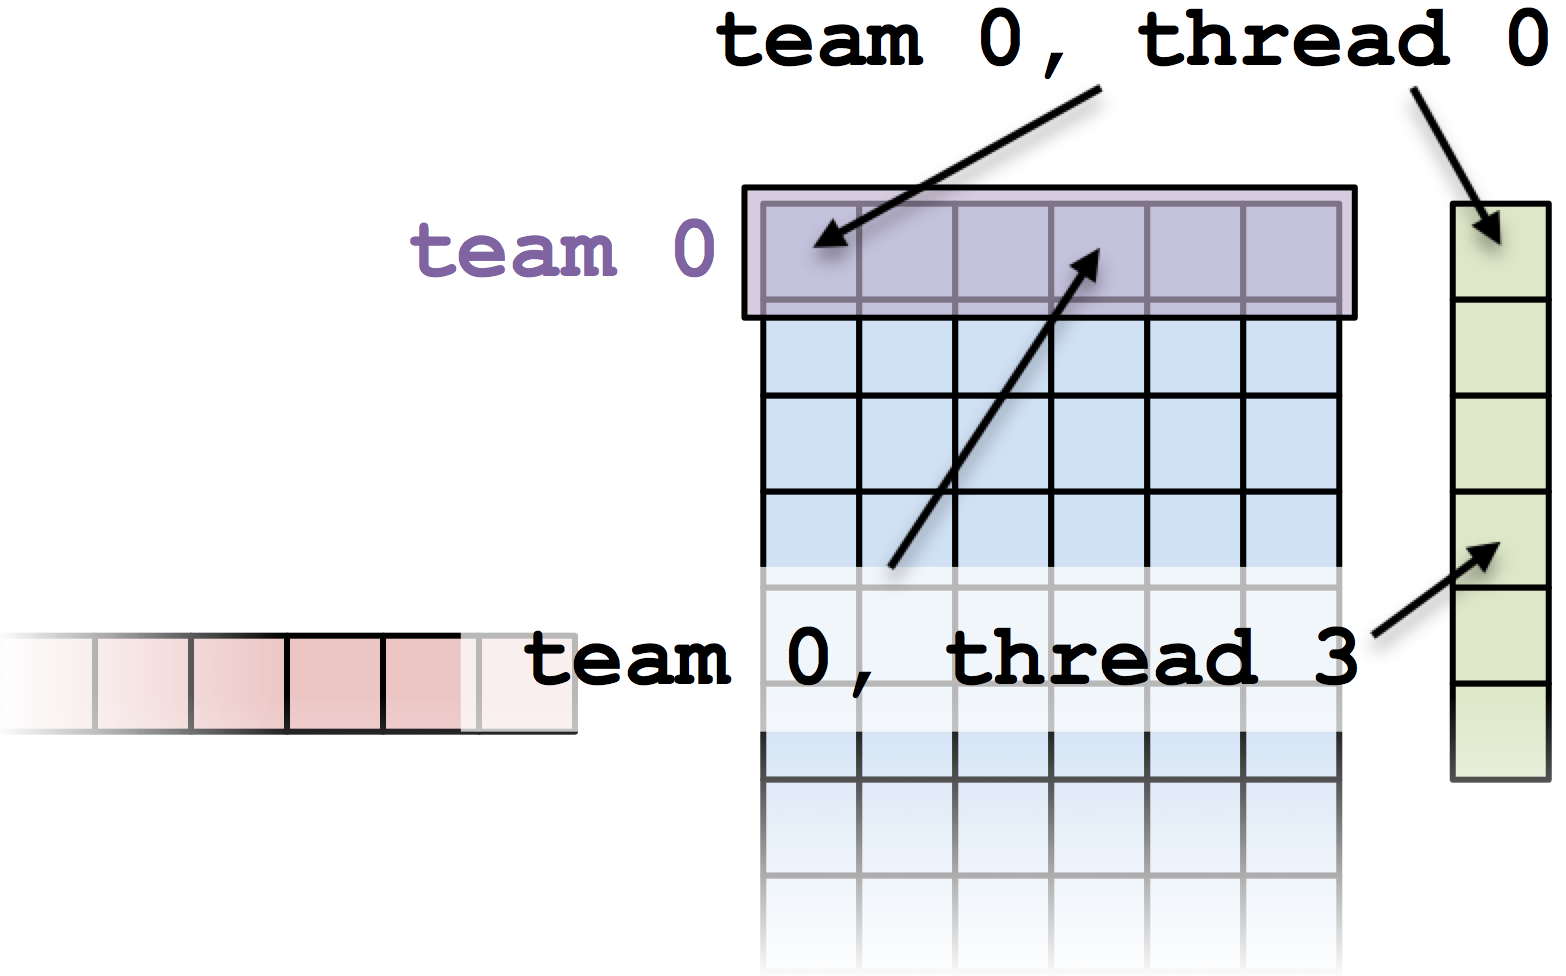
\includegraphics[width=0.53\textwidth]{figures/InnerProductExample_Teams}
      \end{tikzpicture}
      };
  \end{tikzpicture}

  \vspace{50pt}

  First attempt at exercise:

  \begin{code}
@grayoperator() (member_type & teamMember ) {
  const size_t row = teamMember.league_rank();
  const size_t col = teamMember.team_rank();@gray
  atomic_add(&@orangeresult@orange,@darkredy@darkred(row) * @blueA@blue(row,col) * @darkgreenx@darkgreen(entry));
@gray}@gray
  \end{code}

  \pause
  \vspace{-5pt}

  \begin{itemize}

  \item {When team size $\neq$ number of columns, how are units of work mapped to team's member threads?  Is the mapping architecture-dependent?}

  \end{itemize}

\end{frame}
\fi

%==========================================================================

\iffull
\begin{frame}[fragile]{\texttt{TeamThreadRange} (1)}


  Second attempt at exercise:

\vspace{10pt}
  Divide row length among team members.

  \begin{code}
@grayoperator() (member_type & teamMember ) {
  const size_t row = teamMember.league_rank();

  int begin = teamMember.team_rank();
  for(int col = begin; col < M; col += teamMember.team_size()) {
    atomic_add(&@orangeresult@orange, @darkredy@darkred(row) * @blueA@blue(row,col) * @darkgreenx@darkgreen(entry));
  }
@gray}@gray
  \end{code}

  \pause
  \vspace{-5pt}

  \begin{itemize}

  \item {Still bad because \texttt{atomic\_add} performs badly under high contention, how can team's member threads performantly cooperate for a nested reduction?}

  \item {On CPUs you get a bad data access pattern: this hardcodes coalesced access, but not caching.}

  \end{itemize}

\end{frame}
\fi

%==========================================================================

\begin{frame}[fragile]{\texttt{TeamThreadRange} (2)}

  We shouldn't be hard-coding the work mapping...

  \begin{code}[linebackgroundcolor={
        \btLstHL<1->{6}{bodyColor}
      },
      keywords={}
    ]
@grayoperator() (member_type & teamMember, double & update) {
  const int row = teamMember.league_rank();@gray
  double @purplethisRowsSum@purple;
  @pattern``do a reduction''@pattern(@policy``over M columns''@policy,
    [=] (const int col) {
      @purplethisRowsSum@purple += @blueA@blue(row,col) * @darkgreenx@darkgreen(col);
    });
  if (teamMember.team_rank() == 0) {
    update += @darkred@darkred(row) * @purplethisRowsSum@purple;
  }
@gray}@gray
  \end{code}

  \pause
  \vspace{5pt}

  If this were a parallel execution, \\
    \hspace{20pt}we'd use \texttt{Kokkos::parallel\_reduce}.

  \pause
  \vspace{5pt}

  \textbf{Key idea}: this \emph{is} a parallel execution.

  \pause
  \vspace{5pt}

  \hspace{20pt}{\Large $\Rightarrow$ \textbf{Nested parallel patterns}}

\end{frame}

%==========================================================================

\begin{frame}[fragile]{\texttt{TeamThreadRange} (3)}

  \ul{\texttt{TeamThreadRange}:}

  \begin{code}[linebackgroundcolor={
        \btLstHL<1->{6}{bodyColor}
      },
      keywords={}
    ]
@grayoperator() (const member_type & teamMember, double & update ) {
  const int row = teamMember.league_rank();@gray
  double @purplethisRowsSum@purple;
  @patternparallel_reduce@pattern(@policyTeamThreadRange(teamMember, M)@policy,
    [=] (const int col, double & thisRowsPartialSum ) {
      thisRowsPartialSum += @blueA@blue(row, col) * @darkgreenx@darkgreen(col);
    }, @purplethisRowsSum@purple );
  if (teamMember.team_rank() == 0) {
    update += @darkredy@darkred(row) * @purplethisRowsSum@purple;
  }
@gray}@gray
  \end{code}

  \pause

  \begin{itemize}
    \item{The \textbf{mapping} of work indices to threads is \textbf{architecture-dependent}.}
    \item{The \textbf{amount of work} given to the \texttt{TeamThreadRange} \textbf{need not be a multiple} of the \texttt{team\_size}.}
    \item{Intrateam \textbf{reduction handled} by Kokkos.}
  \end{itemize}

\end{frame}

%==========================================================================

\begin{frame}[fragile]{Nested parallelism}

  \ul{\textbf{Anatomy} of nested parallelism:}

  \vspace{-3pt}

  \begin{code}[linebackgroundcolor={
        %\btLstHL<1->{4-7}{bodyColor}
      },
      keywords={}
    ]
@patternparallel_outer@pattern("Label",
  @policyTeamPolicy<ExecutionSpace>(numberOfTeams, teamSize)@policy,
  KOKKOS_LAMBDA (const member_type & teamMember@italic[, ...]@italic) {
    /* beginning of outer body */
    @patternparallel_inner@pattern(
      @policyTeamThreadRange(teamMember, thisTeamsRangeSize)@policy,
      [=] (const unsigned int indexWithinBatch@italic[, ...]@italic) {
        /* inner body */
      }@italic[, ...]@italic);
    /* end of outer body */
  }@italic[, ...]@italic);
  \end{code}

  \vspace{-5pt}

  \begin{itemize}
    \item{\texttt{parallel\_outer} and \texttt{parallel\_inner} may be any combination of \texttt{for} and/or \texttt{reduce}.}
    \item{The inner lambda may capture by reference, but capture-by-value is recommended.}
    \item{The policy of the inner lambda is always a \texttt{TeamThreadRange}.}
    \item{\texttt{TeamThreadRange} cannot be nested.}
  \end{itemize}

\end{frame}

%==========================================================================

\begin{frame}[fragile]{What should the team size be?}

  In practice, you can \textbf{let Kokkos decide}:

    \begin{code}[linebackgroundcolor={
      },
      keywords={}
    ]
parallel_something(
  TeamPolicy<ExecutionSpace>(numberOfTeams, Kokkos::AUTO),
  /* functor */);
    \end{code}

  \pause
  \vspace{0pt}

  \ul{\textbf{GPUs}}

  \begin{itemize}
    \item{Special hardware available for coordination within a team.}
    \item{Within a team 32 (NVIDIA) or 64 (AMD) threads execute ``lock step.''}
    \item{Maximum team size: \textbf{1024}; Recommended team size: \textbf{128/256}}
  \end{itemize}

  \pause
  \vspace{0pt}

  \ul{\textbf{Intel Xeon Phi}:}

  \begin{itemize}
    \item{Recommended team size: \# hyperthreads per core}
    \item{Hyperthreads share entire cache hierarchy} \\
      \hspace{2em}{a well-coordinated team avoids cache-thrashing}
  \end{itemize}

\end{frame}

%==========================================================================

\begin{frame}[fragile]{Exercise: TeamPolicy}

  \textbf{Details}:
  \begin{small}
  \begin{itemize}
\item Location: \ExerciseDirectory{team\_policy}
\item Replace \texttt{RangePolicy<Space>} with \texttt{TeamPolicy<Space>}
\item Use \texttt{AUTO} for \texttt{team\_size}
\item Make the inner loop a \texttt{parallel\_reduce} with \texttt{TeamThreadRange} policy
\item Experiment with the combinations of \texttt{Layout}, \texttt{Space}, \texttt{N} to view performance
\item Hint: what should the layout of \texttt{A} be?
\end{itemize}
  \end{small}

\ul{\textbf{Things to try:}}
  \begin{small}
  \begin{itemize}
  \item Vary problem size and number of rows (-S ...; -N ...)
  \item Compare behavior with Exercise 4 for very non-square matrices
  \item Compare behavior of CPU vs GPU
  \end{itemize}
  \end{small}

\end{frame}

%==========================================================================

\begin{frame}[fragile]{Reminder, Exercise \#4 with Flat Parallelism}

  \vspace{-10pt}

    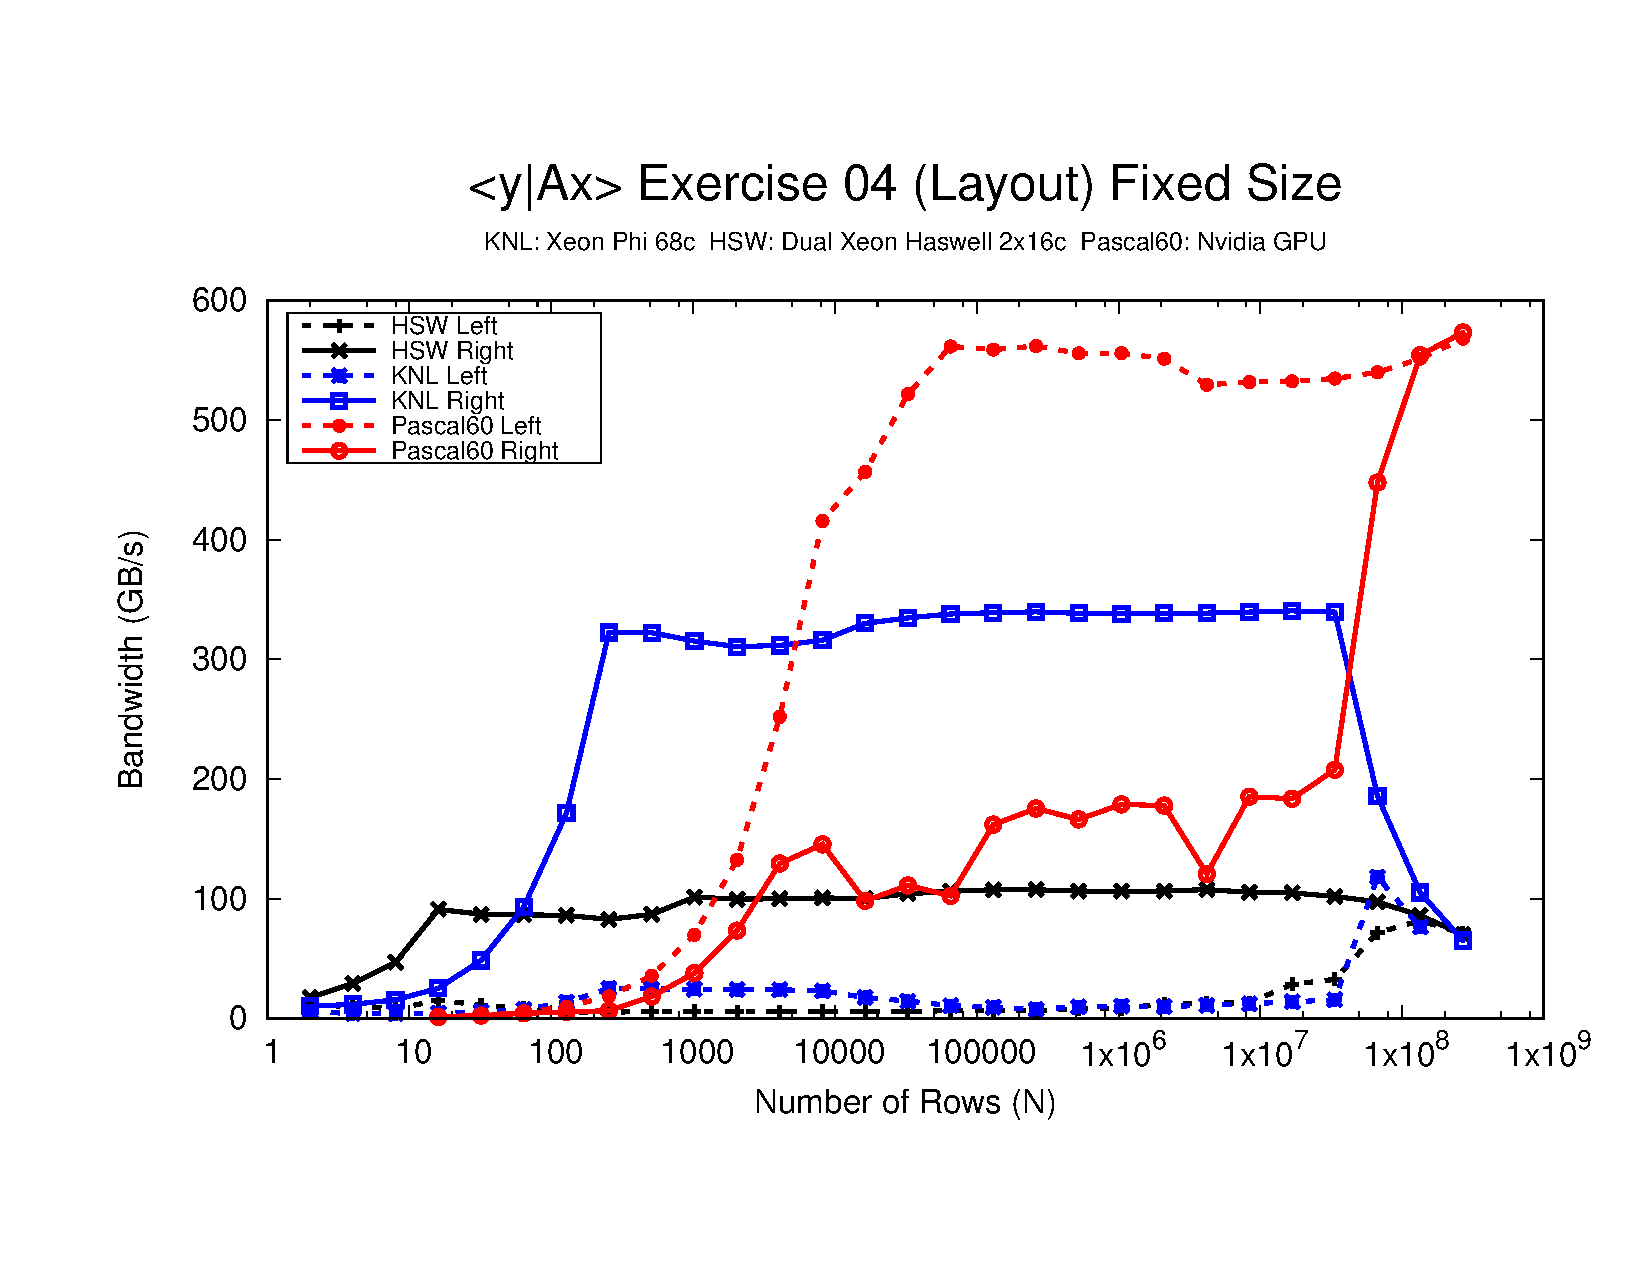
\includegraphics[viewport=1.25in 3.0in 10in 6in, width=0.95\textwidth]{figures/Exercise04-Performance.pdf}

  \vspace{-15pt}

  \begin{textblock*}{0.5\textwidth}(0.65\textwidth,0.28\textheight)
    \textbf{coalesced}
  \end{textblock*}

  \begin{textblock*}{0.5\textwidth}(0.60\textwidth,0.44\textheight)
    \textbf{cached}
  \end{textblock*}

  \begin{textblock*}{0.5\textwidth}(0.60\textwidth,0.61\textheight)
    \textbf{uncoalesced}
  \end{textblock*}

  \begin{textblock*}{0.5\textwidth}(0.70\textwidth,0.68\textheight)
    \textbf{cached}
  \end{textblock*}

  \begin{textblock*}{0.5\textwidth}(0.70\textwidth,0.77\textheight)
    \textbf{uncached}
  \end{textblock*}

\end{frame}

%==========================================================================

\begin{frame}[fragile]{Exercise: TeamPolicy}

  \vspace{-10pt}

  \begin{center}
    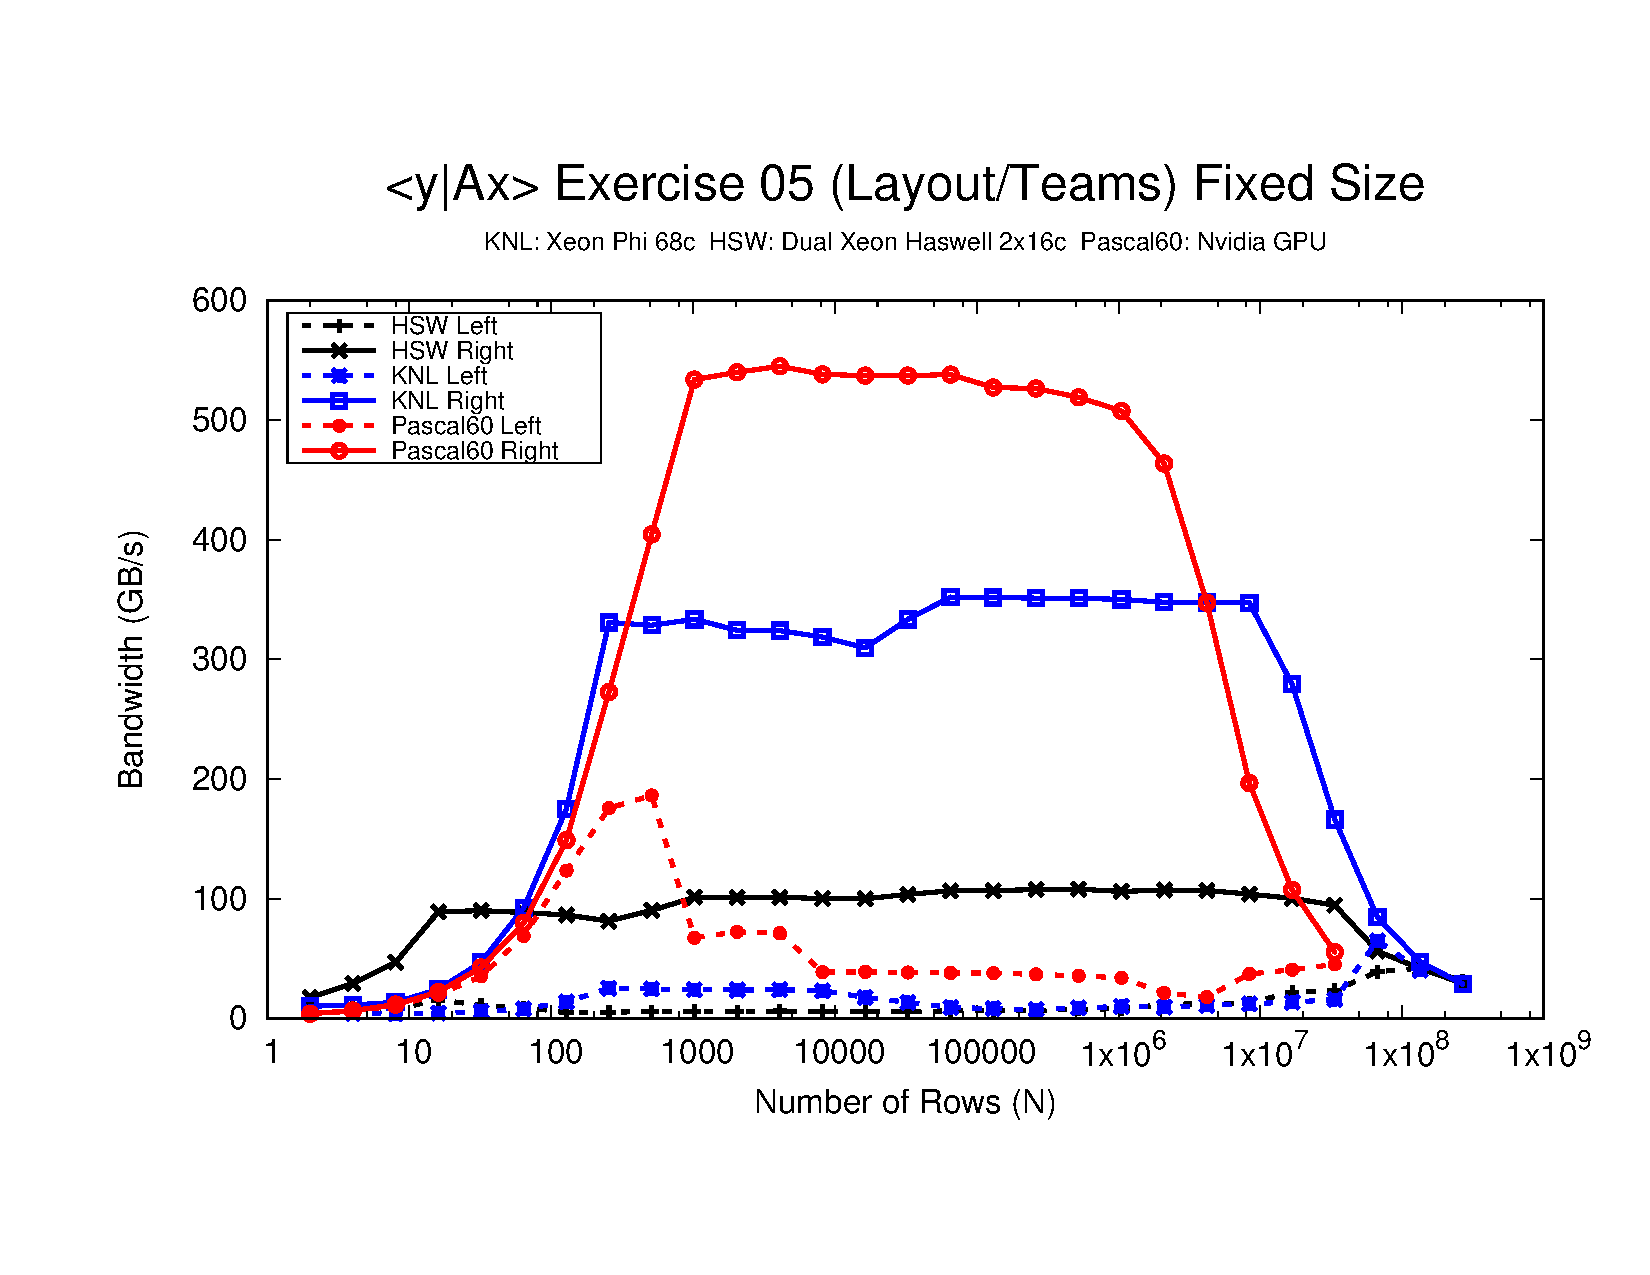
\includegraphics[viewport=1.25in 3.0in 10in 6in, width=0.95\textwidth]{figures/Exercise05-Performance.pdf}
  \end{center}

  \vspace{-15pt}

  \begin{textblock*}{0.5\textwidth}(0.55\textwidth,0.32\textheight)
    \textbf{coalesced}
  \end{textblock*}

  \begin{textblock*}{0.5\textwidth}(0.60\textwidth,0.44\textheight)
    \textbf{cached}
  \end{textblock*}

  \begin{textblock*}{0.5\textwidth}(0.70\textwidth,0.68\textheight)
    \textbf{cached}
  \end{textblock*}

\end{frame}

%==========================================================================

\begin{comment}
\begin{frame}[fragile]{Example: sparse matrix-vector product (0)}

  Sparse matrix \textbf{representation}:

  \vspace{-7pt}

  \begin{table}
    \small
    \begin{tabular}{| l | c | c | c | c | c |}
      \hline
      \texttt{colIndices} & 17 & 45 & 73 & 7 & ... \\
      \hline
      \texttt{colValues} & 3.1 & 4.1 & 5.9 & 2.6 & ...\\
      \hline
      \texttt{irow} & 0 & 3 & 9 & ... & \\
      \hline
    \end{tabular}
  \end{table}

  \vspace{10pt}

  \textbf{Serial} algorithm:

  \vspace{-2pt}

  \begin{code}[linebackgroundcolor={
      },
      keywords={}
    ]
for (row = 0; row < matrixSize; ++row) {
  double total = 0;
  for (int i = irow[row]; i < irow[row+1]; ++i) {
    total += colValues[i] * vec[colIndices[i]];
  }
  product[row] = total;
}
  \end{code}

  \pause
  \vspace{10pt}

  How many ways can this be parallelized?

\end{frame}

%==========================================================================

\begin{frame}[fragile]{Example: sparse matrix-vector product (1)}

  \ul{\textbf{Flat} over \textbf{rows}:}

  \begin{code}[linebackgroundcolor={
      },
      frame=single,
      keywords={}
    ]
operator()(int row) const {
  double total = 0;
  for (int i = _irow(row); i < _irow(row+1); ++i) {
    total += _colValues(i) * _vec(_colIndices(i));
  }
  _product[row] = total;
}
  \end{code}

  \vspace{5pt}

  \begin{itemize}
    \item{One thread \textbf{per row}}
    \item{\texttt{\_colValues} and \texttt{\_colIndices}: {\color{darkgreen}cached}/{\color{darkred}uncoalesced}}
    \item{\texttt{\_vec}: {\color{darkred}uncached}/{\color{darkred}uncoalesced}}
    \item{\texttt{\_product}: {\color{darkgreen}cached}/{\color{darkgreen}coalesced}}
  \end{itemize}

\end{frame}

%==========================================================================

\begin{frame}[fragile]{Example: sparse matrix-vector product (2)}

  \ul{\textbf{Flat} over \textbf{non-zeros} with atomics:}

  \begin{code}[linebackgroundcolor={
      },
      frame=single,
      keywords={}
    ]
operator()(int i) const {
  atomic_add(&_product(_rowIndices(i)),
             colValues(i) * _vec(_colIndices(i)));
}
  \end{code}

  \begin{itemize}
    \item{One thread \textbf{per nonzero entry}}
    \item{\texttt{\_colValues}, \texttt{\_colIndices}, \texttt{\_rowIndices}: {\color{darkgreen}cached}/{\color{darkgreen}coalesced}}
    \item{\texttt{\_vec}: {\color{darkred}uncached}/{\color{darkred}uncoalesced}}
    \item{\texttt{\_product}: {\color{darkgreen}good}/{\color{darkred}bad}}
  \end{itemize}

\end{frame}

%==========================================================================

\begin{frame}[fragile]{Example: sparse matrix-vector product (3)}

  \ul{Hierarchical \textbf{thread teams}:}

  \begin{code}[linebackgroundcolor={
      },
      frame=single,
      keywords={}
    ]
operator()(member_type teamMember) const {
  int row = teamMember.league_rank();
  double total;
  Kokkos::parallel_reduce
    (Kokkos::TeamThreadRange(teamMember, numNonzeros),
     [=] (const unsigned int j, double & valueToUpdate) {
      const unsigned int i = irow(row) + j;
      valueToUpdate += _colValues(i) * _vec(_colIndices(i));
    }, total);
  if (teamMember.team_rank() == 0) {
    _product(row) = total;
  }
}
  \end{code}

  \vspace{-5pt}

  \begin{itemize}
    \item{One thread \textbf{per nonzero entry}}
    \item{\texttt{\_colValues}, \texttt{\_colIndices}: {\color{darkgreen}cached}/{\color{darkgreen}coalesced}}
    \item{\texttt{\_vec}: {\color{darkred}uncached}/{\color{darkred}uncoalesced}}
    \item{\texttt{\_product}: {\color{darkgreen}cached}/{\color{darkgreen}single write}}
  \end{itemize}

\end{frame}

%==========================================================================

\begin{frame}[fragile]{Example: sparse matrix-vector product (4)}

  \ul{\textbf{Performance:}}

  \begin{center}
    \includegraphics[width=1.00\textwidth]{figures/SparseMatrixVectorProduct_summaryNoTexture.pdf}
  \end{center}

\end{frame}

%==========================================================================

\begin{frame}[fragile]{Example: sparse matrix-vector product (5)}

  \ul{\textbf{Performance} (including texture versions):}

  \begin{center}
    \includegraphics[width=1.00\textwidth]{figures/SparseMatrixVectorProduct_summary.pdf}
  \end{center}

\end{frame}
\end{comment}

%==========================================================================

\begin{frame}[fragile]{Three-level parallelism (0)}

  \ul{\textbf{Exposing Vector Level Parallelism}}

  \begin{itemize}
    \item{Optional \textbf{third level} in the hierarchy: \texttt{ThreadVectorRange}}
      \begin{itemize}
        \item{Can be used for \texttt{parallel\_for}, \texttt{parallel\_reduce}, or \texttt{parallel\_scan}.}
      \end{itemize}
    \item{Maps to vectorizable loop on CPUs or (sub-)warp level parallelism on GPUs.}
    \item{Enabled with a \textbf{runtime} vector length argument to \texttt{TeamPolicy}}
    \item{There is \textbf{no} explicit access to a vector lane ID.}
    \item{Depending on the backend the full global parallel region has active vector lanes.}
    \item{\texttt{TeamVectorRange} uses both \textbf{thread} and \textbf{vector} parallelism.}
  \end{itemize}


\end{frame}

%==========================================================================

\begin{frame}[fragile]{Three-level parallelism (1)}

  \ul{\textbf{Anatomy} of nested parallelism:}

  \vspace{-3pt}

  \begin{code}[linebackgroundcolor={
        %\btLstHL<1->{4-7}{bodyColor}
      },
      keywords={}
    ]
@patternparallel_outer@pattern("Label",
  @policyTeamPolicy<>(numberOfTeams, teamSize, vectorLength)@policy,
  KOKKOS_LAMBDA (const member_type & teamMember@italic[, ...]@italic) {
    /* beginning of outer body */
    @patternparallel_middle@pattern(
      @policyTeamThreadRange(teamMember, thisTeamsRangeSize)@policy,
      [=] (const int indexWithinBatch@italic[, ...]@italic) {
        /* begin middle body */
        @patternparallel_inner@pattern(
           @policyThreadVectorRange(teamMember, thisVectorRangeSize)@policy,
           [=] (const int indexVectorRange@italic[, ...]@italic) {
             /* inner body */
           }@italic[, ....);
        /* end middle body */
      }@italic[, ...]@italic);
    @patternparallel_middle@pattern(
    @policyTeamVectorRange(teamMember, someSize)@policy,
      [=] (const int indexTeamVector[, ...]) {
	/* nested body */
      }[, ...]);
    /* end of outer body */
  }@italic[, ...]@italic);
  \end{code}

\end{frame}

%==========================================================================

\ifmedium
\begin{frame}[fragile]{Sum sanity checks (0)}

  \textbf{Question:} What will the value of \texttt{totalSum} be?

  \begin{code}[linebackgroundcolor={}]
int @darkgreentotalSum@darkgreen = 0;
parallel_reduce("Sum", RangePolicy<>(0, numberOfThreads),
  KOKKOS_LAMBDA (size_t& index, int& @darkredpartialSum@darkred) {
    int @bluethisThreadsSum@blue = 0;
    for (int i = 0; i < 10; ++i) {
      ++@bluethisThreadsSum@blue;
    }
    @darkredpartialSum@darkred += @bluethisThreadsSum@blue;
}, @darkgreentotalSum@darkgreen);
  \end{code}

  \pause

  \vspace{15pt}

  \texttt{totalSum = numberOfThreads * 10}

\end{frame}
\fi

%==========================================================================

\ifmedium
\begin{frame}[fragile]{Sum sanity checks (1)}

  \textbf{Question:} What will the value of \texttt{totalSum} be?

  \begin{code}[linebackgroundcolor={}]
@grayint totalSum = 0;
parallel_reduce("Sum", @grayTeamPolicy<>(numberOfTeams, team_size),
  @grayKOKKOS_LAMBDA (@graymember_type& teamMember,@gray int& partialSum) {
    int thisThreadsSum = 0;
    for (int i = 0; i < 10; ++i) {
      ++thisThreadsSum;
    }
    partialSum += thisThreadsSum;
}, totalSum);@gray
  \end{code}

  \pause

  \vspace{15pt}

  \texttt{totalSum = numberOfTeams * team\_size * 10}

\end{frame}
\fi

%==========================================================================

\ifmedium
\begin{frame}[fragile]{Sum sanity checks (2)}

  \textbf{Question:} What will the value of \texttt{totalSum} be?

  \begin{code}[linebackgroundcolor={}]
@grayint totalSum = 0;
parallel_reduce("Sum", TeamPolicy<>(numberOfTeams, team_size),
  KOKKOS_LAMBDA (member_type& teamMember, int& partialSum) {@gray
    int @orangethisTeamsSum@orange = 0;
    parallel_reduce(TeamThreadRange(teamMember, team_size),
      [=] (const int index, int& @purplethisTeamsPartialSum@purple) {
      @grayint thisThreadsSum = 0;
      for (int i = 0; i < 10; ++i) {
        ++thisThreadsSum;
      }@gray
      @purplethisTeamsPartialSum@purple += thisThreadsSum;
    }, @orangethisTeamsSum@orange);
    partialSum += @orangethisTeamsSum@orange;
@gray}, totalSum);@gray
  \end{code}

  \pause

  \vspace{15pt}

  \texttt{totalSum = numberOfTeams * team\_size * team\_size * 10}

\end{frame}
\fi

%==========================================================================

\begin{frame}[fragile]{Restricting Execution: single pattern}
The \texttt{single} pattern can be used to restrict execution
 \begin{itemize}
    \item{Like parallel patterns it takes a policy, a lambda, and optionally a broadcast argument.}
    \item{Two policies: \texttt{PerTeam} and \texttt{PerThread}.}
    \item{Equivalent to OpenMP {\bf single} directive with {\bf nowait}}
 \end{itemize}
\begin{code}[linebackgroundcolor={}]
// Restrict to once per thread
single(PerThread(teamMember), [&] () {
  // code
});

// Restrict to once per team with broadcast
int broadcastedValue = 0;
single(PerTeam(teamMember), [&] (int& broadcastedValue_local) {
	broadcastedValue_local = special value assigned by one;
}, broadcastedValue);
// Now everyone has the special value
\end{code}
\end{frame}

%==========================================================================

\begin{frame}[fragile]{Exercise: TeamVectorLoop}
The previous example was extended with an outer loop over ``Elements'' to expose
a third natural layer of parallelism.

\vspace{10pt}

  \textbf{Details}:
  \begin{small}
  \begin{itemize}
\item Location: \ExerciseDirectory{team\_vector\_loop}
\item Use the \texttt{single} policy instead of checking team rank
\item Parallelize all three loop levels.
\end{itemize}
  \end{small}

\ul{\textbf{Things to try:}}
  \begin{small}
  \begin{itemize}
  \item Vary problem size and number of rows (-S ...; -N ...)
  \item Compare behavior with TeamPolicy Exercise for very non-square matrices
  \item Compare behavior of CPU vs GPU
  \end{itemize}
  \end{small}
\end{frame}

%==========================================================================

\begin{frame}[fragile]{Exercise: TeamVectorLoop}

  %\vspace{-10pt}

    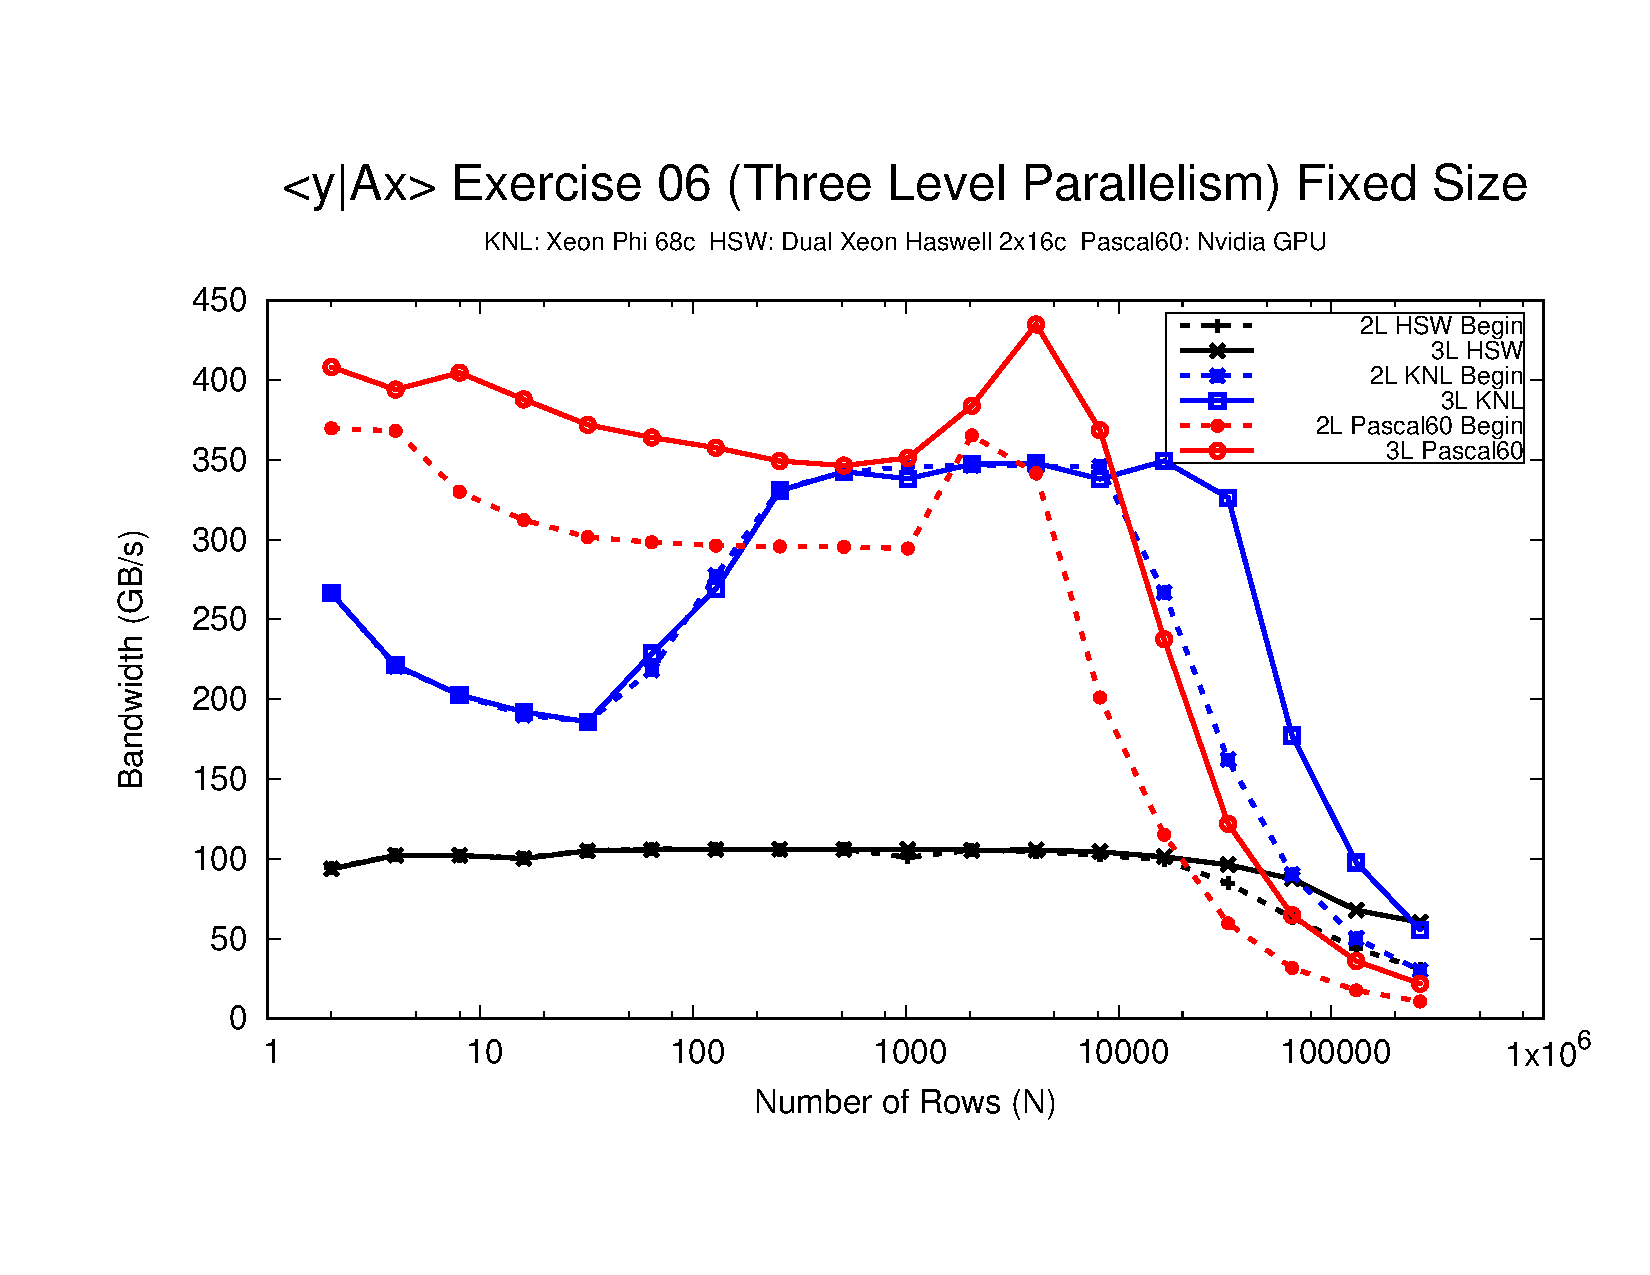
\includegraphics[viewport=1.25in 3.0in 10in 6in, width=0.95\textwidth]{figures/Exercise06-Performance.pdf}

  \vspace{-15pt}

\end{frame}

%==========================================================================

\begin{frame}{Section Summary}

  \begin{itemize}
    \item{\textbf{Hierarchical work} can be parallelized via hierarchical parallelism.}
    \item{Hierarchical parallelism is leveraged using \textbf{thread teams} launched with a \texttt{TeamPolicy}.}
    \item{Team ``worksets'' are processed by a team in nested \texttt{parallel\_for} (or \texttt{reduce} or \texttt{scan}) calls with a \texttt{TeamThreadRange}, \texttt{ThreadVectorRange}, and \texttt{TeamVectorRange} policy.}
    \item{Execution can be restricted to a subset of the team with the \texttt{single} pattern using either a \texttt{PerTeam} or \texttt{PerThread} policy.}
  \end{itemize}

\end{frame}


\begin{frame}[fragile]

  {\Huge Kokkos Tools}

  \vspace{10pt}

  {\large Leveraging Kokkos' built-in instrumentation.}

  \vspace{20pt}

  \textbf{Learning objectives:}
  \begin{itemize}
    \item {The need for Kokkos-aware tools.}
    \item {How instrumentation helps.}
    \item {Simple profiling tools.}
    \item {Simple debugging tools.}
  \end{itemize}

  \vspace{-20pt}

\end{frame}

%==========================================================================

\begin{frame}[fragile]{Profiling C++ Code}
  \textbf{Output from NVIDIA NVProf for Trilinos Tpetra}

  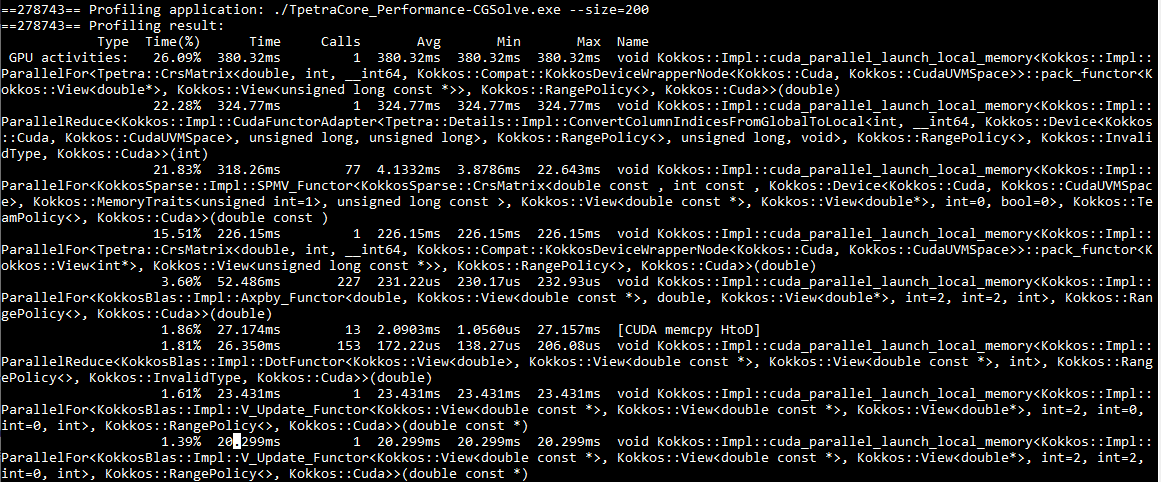
\includegraphics[width=\textwidth]{../figures/tools-tpetra-nvprof}

\vspace{5pt}
\pause
\textit{What are those Kernels doing?}
\end{frame}

%==========================================================================

\begin{frame}[fragile]{Why is it so bad?}
  \textbf{Generic code obscures what is happening from the tools}

  Historically a lot of profiling tools are coming from a Fortran and C world:

  \begin{itemize}
    \item Focused on functions and variables
    \item C++ has a lot of other concepts:
    \begin{itemize}
      \item Classes with member functions
      \item Inheritance
      \item Template Metaprogramming
    \end{itemize}
    \item Abstraction Models (Generic Programming) obscure things
    \begin{itemize}
      \item From a profiler perspective interesting stuff happens in the abstraction layer (e.g. \texttt{\#pragma omp parallel})
      \item Symbol names get really complex due to deep template layers  
    \end{itemize}
  \end{itemize}

\end{frame}

%==========================================================================

\begin{frame}[fragile]{Instrumentation to the Rescue}
  \textbf{Instrumentation enables context information to reach tools.}

  \vspace{5pt}
  Most profiling tools have an instrumentation interface

  \begin{itemize}
    \item E.g. nvtx for NVIDIA, ITT for Intel.
    \item Allows to name regions
    \item Sometimes can mark up memory operations.
  \end{itemize}

  \pause
  \vspace{5pt}
  \begin{block}{KokkosP}
    Kokkos has its own instrumentation interface KokkosP, which can be used to write tools.
  \end{block}

  \begin{itemize}
    \item Knows about parallel dispatch
    \item Knows about allocations, deallocations and deep\_copy
    \item Provides region markers
    \item Leverages naming information (kernels, Views)
  \end{itemize}

\end{frame}

%==========================================================================

\begin{frame}[fragile]{The Kokkos Tools}
  There are two components to Kokkos Tools: the KokkosP instrumentation interface and the actual Tools. 

  \vspace{10pt}
  \textbf{KokkosP Interface}

  \begin{itemize}
    \item The internal instrumentation layer of Kokkos.
    \item Always available even in release builds.
    \item Zero overhead if no tool is loaded.
  \end{itemize}

  \vspace{5pt}
  \textbf{Kokkos Tools}
  \begin{itemize}
    \item Tools leveraging the KokkosP instrumentation layer.
    \item Are loaded at runtime by Kokkos.
    \begin{itemize}
      \item Set \texttt{KOKKOS\_TOOLS\_LIBS} environment variable to load a shared library.
      \item Compile tools into the executable and use the API callback setting mechanism. 
    \end{itemize}
  \end{itemize}
\end{frame}

%==========================================================================

\begin{frame}[fragile]{How does it Work}
Download tools from \url{https://github.com/kokkos/kokkos-tools}

\begin{itemize}
  \item Tools are largely independent of the Kokkos configuration
    \begin{itemize}
      \item May need to use the same C++ standard library.
      \item Use the same tool for CUDA and OpenMP code for example.
     \end{itemize}
  \item We recommend you build the tools with CMake
\begin{lstlisting}
cd kokkos-tools && cmake -B build
cmake --build build --parallel 4
cmake --install build --prefix /where/to/install/the/tools
\end{lstlisting}
\end{itemize}

\vspace{5pt}
Loading Tools:
\begin{itemize}
  \item Set \texttt{KOKKOS\_TOOLS\_LIBS} environment variable to the full path to the shared library of the tool.
  \item Kokkos dynamically loads symbols from the library during \texttt{initialize} and fills function pointers.
  \item If no tool is loaded the overhead is a function pointer comparison to \texttt{nullptr}.
\end{itemize}

\end{frame}



%==========================================================================

\begin{frame}[fragile]{An Example Code}
\begin{code}[keywords={popRegion,pushRegion,Profiling,parallel_for,deep_copy,parallel_scan,parallel_reduce,K_1,K_2,Init_A,tmp,a,h_a}]
View<double*> a("A",N);
View<double*, HostSpace> h_a = create_mirror_view(a);

Profiling::pushRegion("Setup");
parallel_for("Init_A",RangePolicy<h_exec_t>(0,N),
  KOKKOS_LAMBDA(int i) { h_a(i) = i; });
deep_copy(a,h_a);
Profiling::popRegion();

Profiling::pushRegion("Iterate");
for(int r=0; r<10; r++) {
  View<double*> tmp("Tmp",N);
  parallel_scan("K_1",RangePolicy<exec_t>(0,N),
    KOKKOS_LAMBDA(int i, double& lsum, bool f) {
      if(f) tmp(i) = lsum;
      lsum += a(i);
  });
  double sum;
  parallel_reduce("K_2",N, KOKKOS_LAMBDA(int i, double& lsum) {
    lsum += tmp(i);
  },sum);
}
Profiling::popRegion();
\end{code}
\end{frame}

%==========================================================================

\begin{frame}[fragile]{An Example Code: Nvprof}
  Output of: \texttt{nvprof ./test.cuda}

  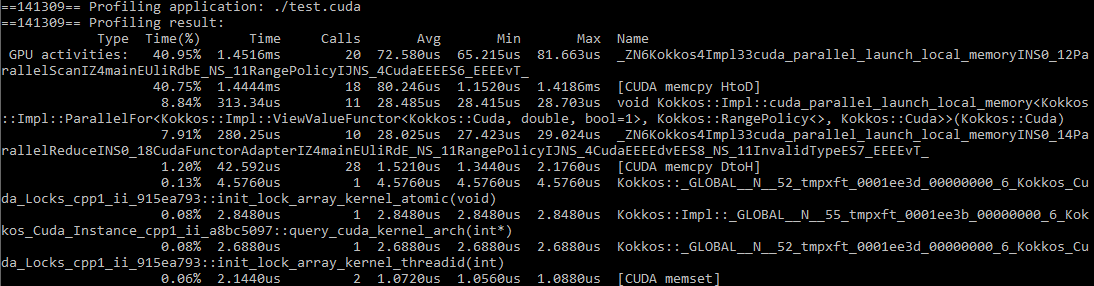
\includegraphics[width=\textwidth]{../figures/tools-nvprof-simple-code}

  \pause
Let us make one larger:

\vspace{-4pt}
\begin{code}
_ZN6Kokkos4Impl33cuda_parallel_launch_local_memoryINS0
_14ParallelReduceINS0_18CudaFunctorAdapterIZ4mainEUliRdE
_NS_11RangePolicyIJNS_4CudaEEEEdvEES8_NS_11InvalidTypeES7_EEEEvT_
\end{code}

And demangled:

\vspace{-4pt}
\begin{code}
void Kokkos::Impl::cuda_parallel_launch_local_memory
<Kokkos::Impl::ParallelReduce<Kokkos::Impl::CudaFunctorAdapter
<main::{lambda(int, double&)#1}, Kokkos::RangePolicy<Kokkos::Cuda>, 
double, void>, Kokkos::Cuda, Kokkos::InvalidType, Kokkos::RangePolicy> >
(Kokkos::Impl::ParallelReduce<Kokkos::Impl::CudaFunctorAdapter<
main::{lambda(int, double&)#1}, Kokkos::RangePolicy<Kokkos::Cuda>, 
double, void>, Kokkos::Cuda, Kokkos::InvalidType, Kokkos::RangePolicy>)
\end{code}
\end{frame}

%==========================================================================

\begin{frame}[fragile]{An Example Code}
\textbf{Aaa this is horrifying can't we do better??}

\pause
\vspace{10pt}
\textbf{Lets use SimpleKernelTimer from Kokkos Tools:}

\begin{itemize}
\item Simple tool producing a summary similar to nvprof
\item Good way to get a rough overview of whats going on
\item Writes a file \texttt{HOSTNAME-PROCESSID.dat} per process
\item Use the reader accompanying the tool to read the data
\end{itemize}

Usage:

\begin{code}[mathescape=false]
  git clone git@github.com:kokkos/kokkos-tools
  cd kokkos-tools/profiling/simple_kernel_timer
  make
  export KOKKOS_TOOLS_LIBS=${PWD}/kp_kernel_timer.so
  export PATH=${PATH}:${PWD}
  cd ${WORKDIR}
  ./text.cuda
  kp_reader *.dat
\end{code}

\end{frame}

%==========================================================================

\begin{frame}[fragile]{An Example Code}

Output from SimpleKernelTimer:
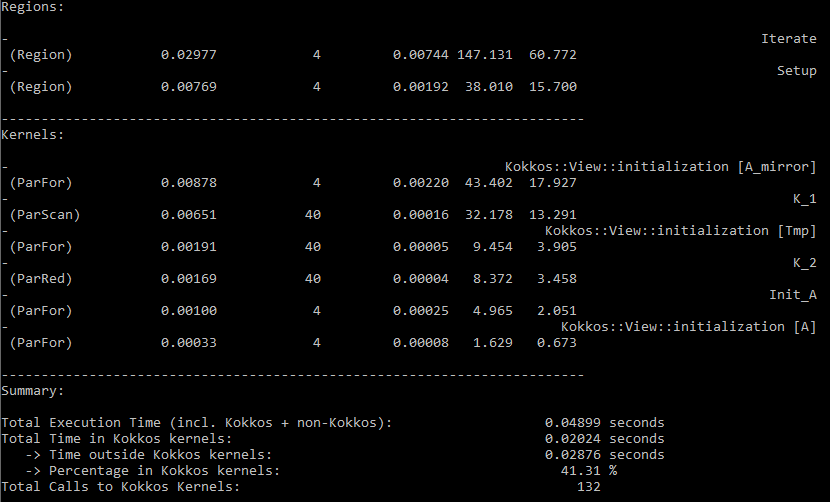
\includegraphics[width=0.85\textwidth]{../figures/tools-kerneltimer-simple-code}

\pause
\vspace{5pt}
Will introduce \textit{Regions} later.

\begin{block}{Kernel Naming}
Naming Kernels avoid seeing confusing Profiler output!
\end{block}

%\begin{code}[keywords={popRegion,pushRegion,Profiling,parallel_for,deep_copy,parallel_scan,parallel_reduce,K_1,K_2,Init_A,tmp,a,h_a}]
%Regions:
%- Iterate (REGION)   0.007105 1 0.007105 202.569506 67.768858
%- Setup (REGION)   0.001906 1 0.001906 54.340290 18.179337
%
%-------------------------------------------------------------------------
%Kernels:
%- K_1 (ParScan)  0.001583 10 0.000158 45.136293 15.100175
%- Kokkos::View::initialization [A_mirror] (ParFor)   0.000809 1 0.000809 23.064374 7.716099
%- Kokkos::View::initialization [Tmp] (ParFor)   0.000419 10 0.000042 11.943444 3.995634
%- K_2 (ParRed)   0.000386 10 0.000039 11.018965 3.686353
%- Init_A (ParFor)   0.000238 1 0.000238 6.784039 2.269575
%- Kokkos::View::initialization [A] (ParFor)   0.000072 1 0.000072 2.052886 0.686785
%
%-------------------------------------------------------------------------
%Summary:
%Total Execution Time (incl. Kokkos + non-Kokkos): 0.01048 s
%Total Time in Kokkos kernels:                     0.00351 s
%   -> Time outside Kokkos kernels:                0.00698 s
%   -> Percentage in Kokkos kernels:               33.45 %
%Total Calls to Kokkos Kernels:                    33
%\end{code}
\end{frame}

%==========================================================================

\begin{frame}[fragile]{Revisiting Tpetra}

Lets look at Tpetra again with the Simple Kernel Timer Loaded:

\vspace{10pt}
At the top we get Region output:

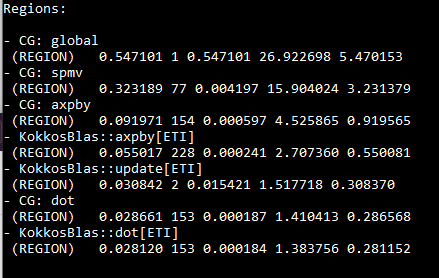
\includegraphics[width=0.7\textwidth]{../figures/tools-tpetra-regions}
\end{frame}

%==========================================================================

\begin{frame}[fragile]{Revisiting Tpetra}


Then we get kernel output:
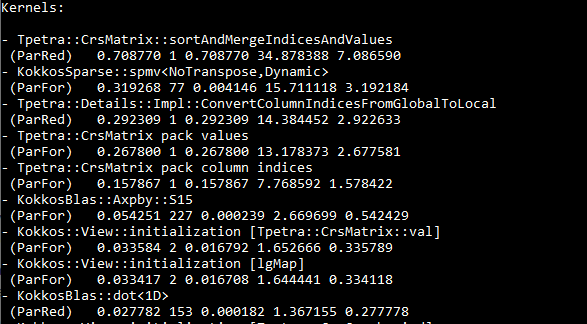
\includegraphics[width=\textwidth]{../figures/tools-tpetra-kernels}
\end{frame}

%==========================================================================

\begin{frame}[fragile]{Memory Utilization}
\textbf{Understanding MemorySpace Utilization is critical}

\vspace{10pt}
Three simple tools for understanding memory utilization:
\begin{itemize}
  \item MemoryHighWaterMark: just the maximum utilization for each memory space.
  \item MemoryUsage: Timeline of memory usage.
  \item MemoryEvents: allocation, deallocation and deep\_copy.
  \begin{itemize}
    \item Name, Memory Space, Pointer, Size
  \end{itemize}
\end{itemize}

\includegraphics[width=0.8\textwidth]{../figures/tools-memevents-simple-code}
\end{frame}

%==========================================================================

\begin{frame}[fragile]{Push/Pop Regions}
	\textbf{Adding region markers to capture more code structure}

Region Markers are helpful to:
\begin{itemize}
  \item Find where time is spent outside of kernels.
  \item Group Kernels which belong together.
  \item Structure code profiles.
  \begin{itemize}
     \item For example bracket \textit{setup} or \textit{solve} phase. 
  \end{itemize}
\end{itemize}

\pause
\vspace{10pt}
Simple Push/Pop interface:
\begin{code}
  Kokkos::Profiling::pushRegion("Label");
  ...
  Kokkos::Profiling::popRegion();
\end{code}
\end{frame}

%==========================================================================

\begin{frame}[fragile]{Space Time Stack}
The simplest tool to leverage regions is the \textbf{Space Time Stack}:

\begin{itemize}
  \item \textbf{Bottom Up} and \textbf{Top Down} data representation
  \item Can do MPI aggregation if compiled with MPI support
  \item Also aggregates memory utilization info.
\end{itemize}

\includegraphics[width=\textwidth]{../figures/tools-sts-bup2-simple-code}

\end{frame}

%==========================================================================

\begin{frame}[fragile]{The Delayed Error Problem}
\textbf{Non-Blocking Dispatch implies asynchronous error reporting!}

\begin{code}[keywords={parallel_for,parallel_reduce,pushRegion,popRegion,Profiling,int,for},linebackgroundcolor={\btLstHL{3-4}{darkred!20}}]
Profiling::pushRegion("Iterate");
for(int r=0; r<10; r++) {
  parallel_for("K_1",2*N, KOKKOS_LAMBDA(int i) {a(i) = i;});  
  printf("Passed point A\n");
  double sum;
  parallel_reduce("K_2",N, KOKKOS_LAMBDA(int i, double& lsum) {
    lsum += a(i); },sum);
}
Profiling::popRegion();
\end{code}

Output of the run:
\begin{code}[linebackgroundcolor={\btLstHL{2}{darkred!20}}]
./test.cuda
Passed point A
terminate called after throwing an instance of 'std::runtime_error'
  what():  cudaStreamSynchronize(m_stream) error( cudaErrorIllegalAddress): 
  an illegal memory access was encountered 
    Kokkos/kokkos/core/src/Cuda/Kokkos_Cuda_Instance.cpp:312
Traceback functionality not available
Aborted (core dumped)
\end{code}
\end{frame}

%==========================================================================

\begin{frame}[fragile]{Kernel Logger for Debugging}
\begin{block}{Debugging with Tools}
Kokkos Tools can be used to implement Debugging functionality.
\end{block}

\pause
The KernelLogger is a tool to localize errors and check the actual runtime flow of a code.
\begin{itemize}
  \item As other tools it inserts fences - which check for errors.
  \item Prints out Kokkos operations as they happen.
\end{itemize}

\pause
Output from the above test case with KernelLogger:

\vspace{-5pt}
\begin{code}
KokkosP: Allocate<Cuda> name: A pointer: 0x7f598b800000 size: 8000000
KokkosP: Executing parallel-for kernel on device 0 with unique execution identifier 0
KokkosP: Kokkos::View::initialization [A]
KokkosP: Execution of kernel 0 is completed.
KokkosP: Entering profiling region: Iterate
KokkosP: Executing parallel-for kernel on device 0 with unique execution identifier 1
KokkosP: Iterate
KokkosP:   K_1
terminate called after throwing an instance of 'std::runtime_error'
  what():  cudaDeviceSynchronize() error( cudaErrorIllegalAddress): an illegal memory access was encountered /ascldap/users/crtrott/Kokkos/kokkos/core/src/Cuda/Kokkos_Cuda_Instance.cpp:143
Traceback functionality not available
\end{code}
\end{frame}

%==========================================================================

\begin{frame}[fragile]{The Standard Profiling Approach}
\textbf{The standard Kokkos profiling approach}

\vspace{10pt}
\textit{Understand Kokkos Utilization (SimpleKernelTimer)}
\begin{itemize}
  \item Check how much time in kernels
  \item Identify HotSpot Kernels
\end{itemize}

\textit{Run Memory Analysis (MemoryEvents)}
\begin{itemize}
  \item Are there many allocations/deallocations - 5000/s is OK.
  \item Identify temporary allocations which could be hoisted
\end{itemize}


\textit{Identify Serial Code Regions (SpaceTimeStack)}
\begin{itemize}
  \item Add Profiling Regions
  \item Find Regions with low fraction of time spend in Kernels
\end{itemize}

\textit{Dive into individual Kernels}
\begin{itemize}
  \item Use connector tools (next subsection) to analyze kernels.
  \item E.g. use roof line analysis to find underperforming code.
\end{itemize}
\end{frame}

%==========================================================================

\begin{frame}[fragile]{Exercise - Terrible MiniMD}
Analyse a MiniMD variant with a serious performance issue.

  \vspace{10pt}

\textbf{Details}:
\begin{small}
\begin{itemize}
  \item Location: \ExerciseDirectory{tools\_minimd}
  \item Use standard Profiling Approach.
  \item Find the code location which causes the performance issue.
  \item Run with \texttt{miniMD.exe -s 20}
\end{itemize}
\end{small}

\ul{\textbf{What should happen:}}
  \begin{small}
  \begin{itemize}
  \item Performance should be
  \item About 50\% of time in a Force compute kernel
  \item About 25\% in neighbor list creation
  \end{itemize}
  \end{small}
\end{frame}

%==========================================================================

\begin{frame}[fragile]{Basic Tool Summary}
\begin{itemize}
  \item Kokkos Tools provide an instrumentation interface \textbf{KokkosP} and \textbf{Tools} to leverage it.
  \item The interface is \textbf{always available} - even in release builds.
  \item Zero overhead if no tool is loaded during the run.
  \item Dynamically load a tool via setting \texttt{KOKKOS\_TOOLS\_LIBS} environment variable.
  \item Set callbacks directly in code for tools compiled into the executable. 
\end{itemize}
\end{frame}




\begin{frame}[fragile]

  {\Huge Kokkos Kernels: performance portable BLAS, sparse, dense and graph algorithms}
  \vspace{20pt}

  \textbf{Topics:}
  \begin{itemize}
    \item {BLAS kernels.}
    \item {SPARSE math kernels.}
  \end{itemize}

  \vspace{-20pt}

\end{frame}

\begin{frame}[fragile]

  {\Huge BLAS and LAPACK}

  \vspace{20pt}

  \textbf{Learning objectives:}
  \begin{itemize}
    \item {Motivation for BLAS/LAPACK functions}
    \item {Algorithm Specialization for Applications}
    \item {Calling BLAS/LAPACK functions}
  \end{itemize}

  \vspace{-20pt}
\end{frame}

%==========================================================================
% Slide 2
\begin{frame}[fragile]{KokkosKernels BLAS/LAPACK Interface}

\vspace{-1em}
  \begin{columns}[t,onlytextwidth]
    \column{.50\textwidth}
      \begin{center}
        \textbf{KokkosKernels}
      \end{center}
    \column{.50\textwidth}
      \begin{center}
        \textbf{Vendor Libraries}
      \end{center}
  \end{columns}

%\noindent\makebox[\linewidth]{\rule{\paperwidth}{0.4pt}}
\noindent\rule{4in}{0.4pt}

  \begin{columns}[t,onlytextwidth]
    \column{.45\textwidth}
      \begin{flushleft}
      \vspace{-2em}
        \begin{itemize}
          \item \small{A single interface to vendor BLAS libraries on
          heterogenous computing platforms}
          \item \small{Support user-defined data type e.g., Automatic Differentiation,
          Ensemble, SIMD, types with Kokkos native implementation}
          \item \small{Customized performance solution for certain problem sizes}
          \item \small{Exploring new performance oriented interfaces}
        \end{itemize}
      \end{flushleft}
    \column{.10\textwidth}
    \column{.45\textwidth}
      \begin{flushright}
      \vspace{-2em}
        \begin{itemize}
          \item \small{A user needs to write a different function interface for
          different computing platforms e.g., MKL vs. CUBLAS}
          \item \small{Built-in real/complex data types and column/row major data
          layouts are only supported}
          \item \small{Code is highly optimized; in practice, higher performance is
          obtained from larger problem sizes}
        \end{itemize}
      \end{flushright}
  \end{columns}
\end{frame}

%==========================================================================
% Slide 3
\begin{frame}[fragile]{KokkosKernels BLAS/LAPACK Interface}
  \textbf{Algorithm Specialization for Applications}
  \begin{itemize}
    \item Dot-based GEMM
    \begin{itemize}
	    \item \small{GEMM is used for orthogonalizing Krylov multi-vectors (long skinny matrix)}
      \item \small{This particular problem shape does not perform well on CUBLAS}
      \item \small{Algorithm is specialized for this shape performing multiple dot
      products instead of running standard GEMM algorithms}
    \end{itemize}
    \item Compact Batched BLAS
    \begin{itemize}
      \item \small{Application wants to solve many instances of tiny square block dense
      matrices; e.g., block dimensions of 3, 5, 7, 9, 11, etc.}
      \item \small{Difficult to effectivley use wide vector length such as AVX512 for
      this small problem size}
      \item \small{A pack of block matrices are inter-leaved and solved simultaneously
      using vector instructions}
      \item \small{Code is trivially vectorized 100\% for the applied BLAS and LAPACK operations}
    \end{itemize}
  \end{itemize}
\end{frame}

%==========================================================================
% Slide 3
\begin{frame}[fragile]{KokkosKernels BLAS/LAPACK Interface}
  \textbf{Algorithm Specialization for Applications}
  \begin{itemize}
    \item Extended Blas 1 interface: see axpby, update (a, c, b, y, g, z)
    \begin{itemize}
      \item $y[i] = g*z[i] + b*y[i] + a*x[i]$
      \item Trilinos Tpetra interface used in Belos iterative solvers
    \end{itemize}
    \item See the wiki page for complete list of functions
    \begin{itemize}
      \item https://github.com/kokkos/kokkos-kernels/wiki
    \end{itemize}
  \end{itemize}
  \vspace{10pt}
  \begin{center}
    \framebox{\parbox[t][1.0cm]{9.0cm}{
      \centering
      \item KokkosKernels interacts with application teams and provides custom 
      performance solutions for their needs
    }}
  \end{center}
\end{frame}

%==========================================================================
% Begin NDE
% Slide 5
\begin{frame}[fragile]{KokkosKernels BLAS/LAPACK Interface}

\textbf {Recall the Kokkos Inner Product exercise:}

\begin{columns}[t,onlytextwidth]
  \column{.50\textwidth}
\begin{itemize}
%  \item Recall the Kokkos Inner Product exercise:
  \item Inner product $<y,A*x>$
  \begin{itemize}
    \item $y$ is $Nx1$, $A$ is $NxM$,\\ $x$ is $Mx1$
  \end{itemize}
  \item Early exercise code looked like

  \begin{code}[keywords={double,parallel_reduce,for,int}]
double result = 0;
Kokkos::parallel_reduce("yAz", N,
    KOKKOS_LAMBDA (int j, double &update) {
      double temp2 = 0;
      for (int i = 0; i < M; ++i) {
        temp2 += A(j, i) * x(i);
      }
      update += y(j) * temp2;
  }, result);
  \end{code}

\end{itemize}

  \column{.50\textwidth}
  \begin{flushright}
    \includegraphics[width=0.85\textwidth]{figures/InnerProductExample_annotated}
  \end{flushright}
\end{columns}
\end{frame}

%Slide 6

\begin{frame}[fragile]{KokkosKernels BLAS/LAPACK Interface}

\textbf {This can be naturally expressed as two BLAS operations:} \\
In Matlab notation:
\vspace{-2em}

\begin{columns}[t,onlytextwidth]
  \column{.50\textwidth}
  \begin{center}
  \begin{code}[keywords={double,parallel_reduce,for,int}]
     // 1. gemv:
     Ytmp = A * x
  \end{code}
  \\
  \includegraphics[width=0.5\textwidth]{figures/BLAS-A_times_x_res}
  \end{center}


  \column{.50\textwidth}
  \begin{center}
  \begin{code}[keywords={double,parallel_reduce,for,int}]
     // 2. dot:
     result = y'*Ytmp
  \end{code}
  \\
  \includegraphics[width=0.5\textwidth]{figures/BLAS-y_dot_tmp}
  \end{center}
\end{columns}
\vspace{5pt}
\small{Different function signatures and APIs are used by different vendors}
\\
\small{  e.g., on Cuda: cublasDgemv and cublasDdot}
\end{frame}

% Slide 7

\begin{frame}[fragile]{KokkosKernels BLAS Interface: GEMV}

%\textbf {KokkosBLAS::gemv}

\begin{code}[basicstyle=\large, keywords={double,gemv,dot}]
KokkosBlas::gemv (mode, alpha, A, x, beta, y);
\end{code}

\textbf {Interface:}

\begin{itemize}
  \item mode [in] 
  \begin{itemize}
    \item "N" for non-transpose
    \item "T" for transpose
    \item "C" for conjugate transpose.
  \end{itemize}
  \item alpha [in] Input coefficient of A*x
  \item A [in] Input matrix, as a 2-D Kokkos::View
  \item x [in] Input vector, as a 1-D Kokkos::View
  \item beta [in] Input coefficient of y
  \item y [in/out] Output vector, as a nonconst 1-D Kokkos::View
\end{itemize}

\end{frame}

% Slide 8

\begin{frame}[fragile]{KokkosKernels BLAS Interface: DOT}

\begin{code}[basicstyle=\large, keywords={double,gemv,dot}]
result = KokkosBlas::dot(x,y);
\end{code}

\textbf {Single Interface:}

\begin{itemize}
  \item x [in] Input vector, as a 1-D Kokkos::View
  \item y [in] Input vector, as a 1-D Kokkos::View
  \item result [out] Scalar result on host
  \item This interface calls Kokkos::fence on all execution spaces
\end{itemize}

\begin{code}[basicstyle=\large, keywords={double,gemv,dot}]
KokkosBlas::dot(r,x,y);
\end{code}

\textbf {Single and Multi-vector Interface:}

\begin{itemize}
  \item x [in] Input (multi-)vector, as a 1-D or 2-D Kokkos::View
  \item y [in] Input (multi-)vector, as a 1-D or 2-D Kokkos::View
  \item r [in/out] Output result, as a rank-0 or 1-D Kokkos::View
  \item This interface is non-blocking.
\end{itemize}

\end{frame}


%==========================================================================
% Slide 9
\begin{frame}[fragile]{KokkosKernels BLAS/LAPACK Interface}

\vspace{-1em}

  \begin{columns}[t,onlytextwidth]
    \column{.50\textwidth}
      \begin{center}
        \textbf{KokkosKernels:}
      \end{center}
    \column{.50\textwidth}
      \begin{center}
        \textbf{User implementation:}
      \end{center}
  \end{columns}

%\noindent\makebox[\linewidth]{\rule{\paperwidth}{0.4pt}}
\noindent\rule{4in}{0.4pt}

  \begin{columns}[t,onlytextwidth]
    \column{.45\textwidth}
      \begin{flushleft}
      \vspace{-2em}
  \begin{code}[keywords={View,double,gemv,dot}, basicstyle=\tiny, breaklines=true]
Kokkos::View<double*> tmp("tmp", N);

KokkosBlas::gemv("N",alpha,A,x,beta,tmp);


double result = 0;

result = KokkosBlas::dot(y,tmp);
  \end{code}
      \end{flushleft}
    \column{.10\textwidth}
    \column{.45\textwidth}
      \begin{flushright}
      \vspace{-2em}
  \begin{code}[keywords={parallel_reduce,for,int,double}, basicstyle=\tiny, breaklines=true]
double result = 0;
Kokkos::parallel_reduce("yAx", N, 
 KOKKOS_LAMBDA (int j, double &update) { 
  double temp2 = 0;
   for (int i = 0; i < M; ++i) { 
     temp2 += A(j, i) * x(i);
   }
   update += y(j) * temp2;
 }, result);
  \end{code}
      \end{flushright}
  \end{columns}

\noindent\rule{4in}{0.4pt}

\vspace{-0.5em}
  \begin{columns}[t,onlytextwidth]
    \column{.45\textwidth}
      \begin{itemize}
        \vspace{-1em}
        \item{\scriptsize{Uses two BLAS functions}}
        \item{\scriptsize{Optionally interface to optimized vendor libraries}}
        \item{\scriptsize{For certain matrix shapes may choose specialized code path for performance}}
      \end{itemize}
    \column{.10\textwidth}
    \column{.45\textwidth}
      \begin{itemize}
        \vspace{-1em}
        \item{\scriptsize{Exploits a single level of parallelism only i.e., internal temp2 is summed sequentially}}
        \item{\scriptsize{Matrix-vector multiplication and dot product are fused in a single kernel}}
      \end{itemize}
  \end{columns}
\vspace{0.5em}
\scriptsize{Related exercise available at: \verb!Exercises/kokkoskernels/InnerProduct!}
%\item \tiny{\url{https://github.com/kokkos/kokkos-tutorials/tree/main/Exercises/kokkoskernels/InnerProduct/Begin}}

\end{frame}

\begin{frame}[fragile]{Summary}

  \textbf{Summary: BLAS/LAPACK}
  \begin{itemize}
  \item \small{Single interface for heterogeneous computing platforms}
  \item \small{Optimized vendor library interface when it is available}
  \item \small{Specialization of algorithms corresponding to application needs}
  \item \small{Native implementation supports strided data layout of a matrix}
  \end{itemize}
  
\end{frame}

%==========================================================================
% End NDE


% Exercise

\begin{frame}[fragile]{Exercise Inner Product Using Kokkos Kernels}

  \begin{small}
  \begin{itemize}
  \item Location: \ExerciseDirectory{kokkoskernels/InnerProduct/Begin}
  \item Assignment: We return to the Inner Product example with two separate sub-exercises:
  \begin{enumerate}
    \item  Use Kokkos Kernels BLAS routines (gemv, dot) to compute the inner product
    \item  Use Kokkos Kernels team-level BLAS routines (dot) within the TeamPolicy implementation within the matrix-vector product calculation
  \end{enumerate}
  \item Compile and run on CPU, GPU; test with NVIDIA's cuBLAS tpl enabled
  \end{itemize}
  \end{small}

\end{frame}

\begin{frame}[fragile]{Exercise Inner Product Using Kokkos Kernels}

  For convenience, use the provided script to install KokkosKernels and generate a Makefile for the exercise

  \begin{code}
    ./run_installlibs_cmake.sh
    make -j
  \end{code}

  Update path and configuration variables in the script as needed based on your based on your setup:

  \begin{scriptsize}
  \begin{itemize}
    \item \textbf{KOKKOS PATH}: Point to your Kokkos source directory
    \item \textbf{KOKKOSKERNELS PATH}: KokkosKernels source directory
    \item \textbf{KOKKOS DEVICES}: Enabled execution spaces
    \item \textbf{TPLS}: Blank by default, optionally set to cublas with Cuda builds
  \end{itemize}
  \end{scriptsize}

  Run exercise

  \begin{code}
    ./innerproduct.exe -S 26
    # Note the warnings, set appropriate environment variables
  \end{code}

  \begin{scriptsize}
  \begin{itemize}
  \item Vary problem size: \textbf{-S \#}
  \item Vary number of rows: \textbf{-N \#}
  \item Vary repeats: \textbf{-nrepeat \#}
  \end{itemize}
  \end{scriptsize}


\end{frame}


\begin{frame}[fragile]

  {\Huge Sparse Linear Algebra}

  \vspace{10pt}

  {\large Sparse linear algebra data structures and functions.}

  \vspace{20pt}

  \textbf{Learning objectives:}
  \begin{itemize}
    \item {Key characteristics algorithms}
    \item {Containers: CrsMatrix, StaticCrsGraph, Vector}
    \item {SpMV}
    \item {SpADD}
    \item {SpGEMM}
  \end{itemize}

  \vspace{-20pt}

\end{frame}

%==========================================================================

\begin{frame}[fragile]{Why do we need this?}
  \textbf{Support for important class of applications}

  \begin{itemize}
  \item Representation of choices for discrete PDE systems (FEM, FD, CVFEM, ...)
  \item Natural use for network representation
    \begin{itemize}
    \item Electrical grid, electronic circuit
    \item Social network
    \end{itemize}
  \end{itemize}


  \begin{block}{Unique format supported: Compressed row sparse}
    Sparse matrices can be stored in various format, currently only Crs format is fully supported, BlockCrs is partially supported
  \end{block}
\end{frame}

\begin{frame}[fragile]{Algorithmic characteristics}
\textbf{Constraints from Crs format}

\begin{itemize}
\item hard to optimize memory access patterns
\item often multi-pass algorithms required
  \begin{enumerate}
  \item compute storage
  \item compute column index and actual values
  \end{enumerate}
\item typically algorithms can be split in symbolic and numeric phases
\end{itemize}

\begin{block}{Symbolic/Numeric split}
  While extremely useful for reuse it is potentially slower for single use case depending on implementation
\end{block}
\end{frame}

\begin{frame}[fragile]{KokkosKernels Handle}
\textbf{Handle: hiding important details!}

\begin{itemize}
\item What the handles does for you:
  \begin{itemize}
  \item stores user parameters
  \item keeps temporary data needed in numeric of solve/apply phases
  \item cleans up temporary data at destruction
  \item contains kernel specific "sub-handle"
  \item specifies required data types
  \end{itemize}

\item Usage: \texttt{KokkosKernels::Experimental::\\ KokkosKernelsHandle<size\_type,\\
  \hspace{3.8cm} index\_type,\\
  \hspace{3.8cm} scalar\_type,\\
  \hspace{3.8cm} ExecutionSpace,\\
  \hspace{3.8cm} TempMemSpace,\\
  \hspace{3.8cm} PermMemSpace>()}
\end{itemize}
\end{frame}

\begin{frame}[fragile]{Containers}

\textbf{One dense structure:}
\begin{itemize}
\item \texttt{View} (of rank 1): represents a "vector"
\item \texttt{View} (of rank 2): represents a "multi-vector"
\end{itemize}

\vspace{1em}
\textbf{Two sparse structures:}
\begin{itemize}
  \item \texttt{StaticCrsGraph}: encodes the sparsity pattern in \texttt{row\_map} and \texttt{entries}
  \item \texttt{CrsMatrix}: contains a \texttt{StaticCrsGraph} and \texttt{values}
\end{itemize}

\vspace{1em}
\textbf{Example:}
\texttt{example/wiki/sparse/KokkosSparse\_wiki\_crsmatrix.cpp}
\end{frame}

\begin{frame}{Sparse kernels interfaces}
  \textbf{Two interfaces for one kernel?}
  \begin{enumerate}
  \item Simplified interface
    \begin{itemize}
    \item uses high level containers
    \item reduced number of parameters and templates
    \item allocates memory
    \end{itemize}
  \item Expert interface
    \begin{itemize}
    \item uses low level container (i.e. views)
    \item allows for finer memory management
    \end{itemize}
  \end{enumerate}

\begin{block}{Simplified/Expert interface}
  For clarity we will focus on the simplified interface in the rest of the lecture
\end{block}
\end{frame}

\begin{frame}[fragile]{SpMV}
  \textbf{SpMV: a mixed sparse/dense kernel}

  \begin{equation*}
  0.5*\begin{bmatrix}
    4\\ 5\\ 6\\
  \end{bmatrix}+1.0
  \begin{bmatrix}
    1 & & 2 \\
    & 3 & \\
    4 & & 5 \\
  \end{bmatrix}
  \begin{bmatrix}
    1\\ 2\\ 3\\
  \end{bmatrix}
  =\begin{bmatrix}
  9 \\ 8.5 \\ 22
  \end{bmatrix}
  \end{equation*}
  
  \begin{itemize}
  \item Computes: $y = \beta*y + \alpha*A*x$
  \item Output is a dense vector
    \begin{itemize}
    \item single pass algorithm since no CrsGraph needs to be computed
    \item good amount of parallelism exploitable
    \end{itemize}
  \item Usage:  \\ \hspace{1em}\texttt{KokkosSparse::spmv(mode, alpha, A, x, beta, y);}
  \item Example:\\ \hspace{1em}\texttt{example/wiki/sparse/KokkosSparse\_wiki\_spmv.cpp}
  \end{itemize}
\end{frame}

\begin{frame}[fragile]{SpADD}
  \textbf{SpADD: Sparse Matrix Addition}
    \begin{equation*}
      2.0\begin{bmatrix}
        1 &   & 2 \\
          & 3 & 4 \\
        5 &   &   \\
      \end{bmatrix}
      +0.5\begin{bmatrix}
      6 &  7 &  \\
        &  8 &  \\
        &    & 9\\
      \end{bmatrix}
      =\begin{bmatrix}
       5 & 3.5 &   4\\
         &  10 &   8\\
      10 &     & 4.5\\
      \end{bmatrix}
    \end{equation*}
  
  \begin{itemize}
  \item Computes: $C=\alpha A + \beta B$ given $A$ and $B$ two CrsMatrices
  \item Sorted inputs speeds-up the kernel and reduces memory consumption
  \item Usage:\\
    \hspace{1em} \texttt{KokkosSparse::spadd\_symbolic(handle, A, B, C);}\\
    \hspace{1em} \texttt{KokkosSparse::spadd\_numeric(handle, alpha, A, beta, B, C);}
  \item Example:\\
    \hspace{1em} \texttt{example/wiki/sparse/KokkosSparse\_wiki\_spadd.cpp}
  \end{itemize}
\end{frame}


\begin{frame}[fragile]{SpGEMM}
\textbf{SpGEMM: Sparse General Matrix Matrix Multiply}
 
\vspace{.4cm}

\begin{itemize}

  \item Compute $A\times B=C$ for given sparse matrices $A$ and $B$
  \begin{equation*}
  \left[ 
  \begin{tabular}{ccc}
	1 &    & 2 \\
   	   & 3 & 4 \\
        5 &    & 
  \end{tabular}
  \right]
  \times
  \left[ 
  \begin{tabular}{r r r r}
	6 &    & 7 & \\
   	8 & 9 &    & \\
           &    &10&11 
  \end{tabular}
  \right] 
  =
    \left[ 
  \begin{tabular}{r r r r}
	  6 &      & 27 & 22 \\
   	24 & 27 & 40 & 41 \\
        30 & 35 &      &      \\ 
  \end{tabular}
  \right]   
\end{equation*}
  \begin{itemize}
     \item Sparsity structure of $C$ is not known in advance!
  \end{itemize}
  
  \vspace{.4cm}
  
  \item We have a two-phase implementation:
  \begin{itemize}
    \item This allows determining the sparsity of $C$ efficiently
  \end{itemize}
 \end{itemize}  
\end{frame}

\begin{frame}[fragile]{SpGEMM}
\textbf{SpGEMM: Sparse General Matrix Matrix Multiply}

\vspace{.4cm}

\begin{itemize}
\item \textbf{Symbolic phase:} 
  \begin{itemize} 
  \item \texttt{KokkosSparse::spgemm\_symbolic(handle, \\ 
    \hspace{2.9cm}A, isTrnspsdA, B, isTrnspsdB, C);} 
  \item determines number of nonzeros in each row of $C$ and
  \item allocates memory for column indices and values of the nonzeros
  \end{itemize} 

  \vspace{.4cm}

\item \textbf{Numeric phase}
  \begin{itemize}
  \item \texttt{KokkosSparse::spgemm\_numeric(handle, \\ 
    \hspace{2.7cm}A, isTrnspsdA, B, isTrnspsdB, C);}
  \item computes column indices and values of the nonzeros of $C$
  \end{itemize}

  \vspace{.4cm}

\item \textbf{Example}\\[-3ex]
  \hspace{1em} \texttt{example/wiki/sparse/KokkosSparse\_wiki\_spgemm.cpp}
\end{itemize}  
\end{frame}


\begin{frame}[fragile]{SpGEMM}
\textbf{SpGEMM: Sparse General Matrix Matrix Multiply}

\begin{itemize}

  \item We follow Gustavson's algorithm: \\
   \hspace{0.4cm}   \textbf{for} each row index $i\gets 0$  \textbf{to} $nrowsA$ \textbf{do} \\
   \hspace{0.8cm} 	   \textbf{for} each column index $j\in A(i,:)$ \textbf{do} \\
   \hspace{1.2cm}	     	//\texttt{accumulate partial row results}\\
   \hspace{1.2cm}	     	$C(i,:) \gets C(i,:) + A(i,j)B(j,:)$
   
  \vspace{.4cm}
  \item Our implementation exploits hierarchical paralelism
  \begin{itemize}
  	\item Teams are assigned contiguous row chunks in $A$  
      	\item Threads are assigned individual rows of $A$
        \item Vector lanes are assigned the nonzeros of rows of $B$
  \end{itemize} 


 \end{itemize}  
\end{frame}

\begin{frame}[fragile]{SpGEMM}
\textbf{SpGEMM: Sparse General Matrix Matrix Multiply}

\begin{itemize}
  \item We follow Gustavson's algorithm: \\
   \hspace{0.4cm}   \textbf{for} each row index $i\gets 0$  \textbf{to} $nrowsA$ \textbf{do} \\
   \hspace{0.8cm} 	   \textbf{for} each column index $j\in A(i,:)$ \textbf{do} \\
   \hspace{1.2cm}	     	//\texttt{accumulate partial row results}\\
   \hspace{1.2cm}	     	$C(i,:) \gets C(i,:) + A(i,j)B(j,:)$
  \item Our thread-scalable hashmap accumulator implementation
  \begin{itemize} 
    	\item is used in both symbolic and numeric phases
  	\item supports both sparse and dense accumulators
	\item has a two-level structure: Level-1 ($L_1$) and Level-2 ($L_2$)
	\begin{itemize}
	  \item $L_1$ hashmap lives in the fast shared memory
	  \item $L_2$ hashmap is created only if $L_1$ hashmap runs out of memory
	  \item $L_2$ hashmap lives in the large global memory 
	\end{itemize}
  \end{itemize}
  \item For more details see: {\footnotesize M. Deveci, C. Trott, S. Rajamanickam, "Multithreaded sparse matrix-matrix multiplication for many-core and GPU architectures", Parallel Computing 78, 33-46, 2018.}
 \end{itemize}  
\end{frame}

\begin{frame}[fragile]{Summary SpLA}

  \textbf{Summary: Sparse Linear Algebra}
  \begin{itemize}
    \item {Main difficulties: finding sparsity patterns and memory access}
    \item {Containers: \texttt{View}, \texttt{StaticCrsGraph} and \texttt{CrsMatrix}}
    \item {Kernels: SpMV, SpADD and SpGEMM}
  \end{itemize}

\end{frame}


\begin{frame}[fragile]{What we didn't cover}
	\textbf{This was a short introduction}
	
	Didn't cover many things:
	\begin{itemize}
		\item<2-> Full BuildSystem integration.
%		\item<3-> Non-Sum reductions / multiple reductions.
%		\item<4-> Multidimensional loops.
		\item<3-> Advanced data structures.
%		\item<6-> Subviews.
		\item<4-> Atomic operations and Scatter Contribute patterns.
		\item<5-> Team Scratch memory (GPU shared memory).
		\item<6-> SIMD vectorization.
		\item<7-> MPI and PGAS integration.
		\item<8-> All Tools for Profiling, Debugging and Tuning.
    \item<9-> All Math Kernels (Batched BLAS, Graphs, Sparse Solvers.
	\end{itemize}

\end{frame}

\begin{frame}{The Kokkos Lectures}
        
	\begin{block}{The Kokkos Lectures}
		Join The Kokkos Lectures for all of those and more in-depth explanations or do them on your own.
	\end{block}

\begin{itemize}
	\item Module 1: Introduction, Building and Parallel Dispatch
	\item Module 2: Views and Spaces
	\item Module 3: Data Structures + MultiDimensional Loops
	\item Module 4: Hierarchical Parallelism
	\item Module 5: Tasking, Streams and SIMD
	\item Module 6: Internode: MPI and PGAS
	\item Module 7: Tools: Profiling, Tuning and Debugging
	\item Module 8: Kernels: Sparse and Dense Linear Algebra
\end{itemize}
\end{frame}

\begin{frame}{Find More}

\textbf{Online Resources}:

\begin{itemize}
        \item \url{https://github.com/kokkos}:
                \begin{itemize}
                        \item Primary Kokkos GitHub Organization
                \end{itemize}
        \item \url{https://github.com/kokkos/kokkos-tutorials/wiki/Kokkos-Lecture-Series}:
                \begin{itemize}
			\item{Slides, recording and Q\&A for the Full Lectures}
                \end{itemize}
        \item \url{https://github.com/kokkos/kokkos/wiki}:
                \begin{itemize}
                        \item Wiki including API reference
                \end{itemize}
        \item \url{https://kokkosteam.slack.com}:
                \begin{itemize}
                        \item Slack channel for Kokkos.
                        \item Please join: fastest way to get your questions answered.
                        \item Can whitelist domains, or invite individual people.
                \end{itemize}
\end{itemize}

\end{frame}

\end{document}

